%% UP THESIS STYLE for LaTeX2e
%% how to use upteses for MIMED dissertations
%%
%% PLEASE send improvements to jlopes at fe.up.pt and to jcf at fe.up.pt
%%

%%========================================
%% Commands: pdflatex thesis
%%           bibtex thesis
%%           makeindex thesis (only if creating an index) 
%%           pdflatex thesis
%% Alternative:
%%          latexmk -pdf thesis.tex
%%========================================

\documentclass[11pt,a4paper,twoside,openright]{report}
\usepackage[utf8]{inputenc}

%\usepackage{sectsty}
%\usepackage{blindtext}

% Headings setup (sectsty)
%\allsectionsfont{helvetica}


%\usepackage[latin1]{inputenc}
%\usepackage[acronym]{glossaries}
\usepackage[nonumberlist, nogroupskip]{glossaries}
\usepackage{lettrine}
%\usepackage[backref=page]{hyperref}
\usepackage{adforn}

\usepackage[backend=biber, style=numeric,maxbibnames=7,sorting=none]{biblatex}
\addbibresource{references.bib}
\addbibresource{full-thesis.bib}
%%%%%%% English version 

%% MIMED options
\usepackage[mimed]{styles/upteses}                   % work version
%\usepackage[mimed,juri]{styles/upteses}             % juri verrion
%\usepackage[mimed,final]{styles/upteses}            % final version

%% Additional options for upteses.sty: 
%% - portugues: titles, etc in portuguese
%% - onpaper: links are not shown (for paper versions)
%% - backrefs: include back references from bibliography to citation place

%%%%%%% Portuguese version

%\usepackage[mimed,portugues]{upteses}        % work version
%\usepackage[mimed,portugues,juri]{upteses}   % juri version
%\usepackage[mimed,portugues,final]{upteses}  % final version

%\usepackage{pdfpages}

%% Uncomment the next lines if side by side graphics used
%\usepackage[lofdepth,lotdepth]{subfig}
%\usepackage{datagidx}
\usepackage{longtable}
\usepackage{xltabular}
\usepackage[inline]{enumitem}
\usepackage{verbatimbox}
\usepackage{lscape} 
\usepackage{makecell}
\usepackage[svgnames, table]{xcolor}
\usepackage{courier}
\usepackage{textcomp}%
\usepackage{manyfoot}%
\usepackage{booktabs}%
\usepackage{footnote}
\usepackage{color,soul}
\usepackage{algorithm2e}
\usepackage{array}
\usepackage{xurl}
\usepackage{caption}
\usepackage{colortbl}
\usepackage{float}
\usepackage{subcaption}
%%%% similarity
\usepackage{calligra}

\usepackage{graphicx}%
\usepackage{multirow}%
\usepackage{amsmath,amssymb,amsfonts}%
\usepackage{amsthm}%
\usepackage{mathrsfs}%
\usepackage[title]{appendix}%
\usepackage{xcolor}%
\usepackage{listings}%
\usepackage{tabularx}
\usepackage{acro}
\usepackage{setspace}
%% Include color package
\usepackage{color}
\definecolor{cloudwhite}{cmyk}{0,0,0,0.025}
\usepackage{enumitem}
\usepackage[helvetica]{quotchap}  % the quotchap package to get fancy chapter styles
\usepackage{titlesec}
\usepackage{adjustbox}

%% lulatex
\usepackage{luatex85}
\usepackage{csquotes}
%% end lualatex

%\usepackage{ebgaramond} % Load Garamond font
\titleformat*{\section}{\sffamily\Large\bfseries}
\titleformat*{\subsection}{\sffamily\large\bfseries}
\titleformat*{\subsubsection}{\sffamily\normalsize\bfseries}
%\fancyhead[LO]{\sffamily \nouppercase{\rightmark}}  % Use Helvetica for headers
%\fancyhead[RE]{\sffamily \nouppercase{\leftmark}}

\renewcommand*{\sectfont}{\fontfamily{phv}\bfseries\Large}  % 'phv' is Helvetica


%% Include source-code listings package
\usepackage{listings}
\lstset{ %
 language=C,                        % choose the language of the code
 basicstyle=\footnotesize\ttfamily,
 keywordstyle=\bfseries,
 numbers=left,                      % where to put the line-numbers
 numberstyle=\scriptsize\texttt,    % the size of the fonts that are used for the line-numbers
 stepnumber=1,                      % the step between two line-numbers. If it's 1 each line will be numbered
 numbersep=8pt,                     % how far the line-numbers are from the code
 frame=tb,
 float=htb,
 aboveskip=8mm,
 belowskip=4mm,
 backgroundcolor=\color{cloudwhite},
 showspaces=false,                  % show spaces adding particular underscores
 showstringspaces=false,            % underline spaces within strings
 showtabs=false,                    % show tabs within strings adding particular underscores
 tabsize=2,	                    % sets default tabsize to 2 spaces
 captionpos=b,                      % sets the caption-position to bottom
 breaklines=true,                   % sets automatic line breaking
 breakatwhitespace=false,           % sets if automatic breaks should only happen at whitespace
 escapeinside={\%*}{*)},            % if you want to add a comment within your code
 morekeywords={*,var,template,new}  % if you want to add more keywords to the set
}

%% Uncomment to create an index (at the end of the document)
%\makeindex

%% Path to the figures directory
%% TIP: use folder ``figures'' to keep all your figures
\graphicspath{{figures/}}

%%----------------------------------------
%% TIP: if you want to define more macros, use an external file to keep them


%%----------------------------------------
%% singular %%


\DeclareAcronym{fhir}{
short = FHIR ,
long = Fast Healthcare Interoperability Resources
}

\DeclareAcronym{hl7}{
short = HL7 ,
long = Health Level Seven
}
\DeclareAcronym{ehr}{
short = EHR,
long = Electronic Health Record
}

\DeclareAcronym{ai}{
short = AI,
long = Artificial Intelligence
}

\DeclareAcronym{api}{
short = API,
long = Application Programming Interface
}

\DeclareAcronym{auroc}{
short = AUROC,
long = Area Under the Receiver Operating Characteristic Curve 
}
\DeclareAcronym{roc}{
short = ROC,
long =  Receiver Operating Characteristic 
}


\DeclareAcronym{bmi}{
short = BMI,
long = Body Mass Index
}

\DeclareAcronym{iqr}{
short = IQR ,
long = Inter-Quartile Range
}
\DeclareAcronym{gan}{
short = GAN ,
long = Generative Adversarial Network
}

\DeclareAcronym{jsd}{
short = JSD ,
long = \textit{Jensen-Shannon Divergence}
}
\DeclareAcronym{ks}{
short = KS ,
long = \textit{Kolmogorov-Smirnov}
}

\DeclareAcronym{auprc}{
short = AUPRC ,
long = Area Under the Precision Recall Curve 
}

\DeclareAcronym{mre}{
short = MRE ,
long = Mean Relative Error
}

\DeclareAcronym{pca}{
short = PCA ,
long = Principal Component Analysis
}
\DeclareAcronym{ml}{
short = ML,
long = Machine Learning
}
\DeclareAcronym{gdpr}{
short = GDPR,
long = General Data Protection Regulation
}

\DeclareAcronym{eu}{
short = EU,
long = European Union
}

\DeclareAcronym{hipaa}{
short = HIPAA,
long = Health Insurance Portability and Accountability Act
}
\DeclareAcronym{his}{
short = HIS,
long = Health Information System
}

\DeclareAcronym{NDCG}{
short = NDCG,
long = Normalized Discounted Cumulative Gain
}

\DeclareAcronym{DCG}{
short = DCG,
long = Discounted Cumulative Gain 
}

\DeclareAcronym{IDCG}{
short = IDCG,
long = Ideal Discounted Cumulative Gain
}

\DeclareAcronym{rbo}{
short = RBO,
long = Rank-biased overlap
}
\DeclareAcronym{IKNL}{
short = IKNL,
long = Integraal Kankercentrum Nederland
}

\DeclareAcronym{MHRA}{
short = MHRA,
long = Healthcare Products Regulatory Agency
}


\DeclareAcronym{us}{
short = USA,
long = United States of America
}

\DeclareAcronym{svm}{
short = SVM,
long = Support Vector Machines
}

\DeclareAcronym{smote}{
short = SMOTE,
long = Synthetic Minority Oversampling Technique
}
\DeclareAcronym{rmse}{
short = RMSE,
long = Root Mean Squared Error
}

\DeclareAcronym{mae}{
short = MAE,
long = Mean Absolute Error
}


\DeclareAcronym{cv}{
short = CV,
long = Cross-Validation
}

\DeclareAcronym{wcss}{
short =  WCSS,
long = within-cluster sum of squares
}

\DeclareAcronym{ri}{
short =  RI,
long =  Rand Index
}
\DeclareAcronym{cs}{
short =  C-Section,
long =  Cesarean Section
}
\DeclareAcronym{knn}{
short =  KNN,
long =  K-Nearest Neighbours
}

\DeclareAcronym{atc}{
short =  ATC,
long =  Anatomical Therapeutic Chemical
}

\DeclareAcronym{kdd}{
short =  KDD,
long =  Knowledge Discovery in Databases
}

\DeclareAcronym{ebm}{
short =  EBM,
long =  Evidence Based Medicine
}
\DeclareAcronym{rct}{
short =  RCT,
long =  Randomized Clinical Trial
}
\DeclareAcronym{rwd}{
short =  RWD,
long =  Real World Data
}
\DeclareAcronym{xai}{
short =  XAI,
long =  Explainable AI
}
\DeclareAcronym{shap}{
short =  SHAP,
long =  SHapley Additive exPlanations
}


\DeclareAcronym{lime}{
short =  LIME,
long =  Local Interpretable Model-Agnostic Explanation
}
\DeclareAcronym{bn}{
short =  BN,
long =  Bayesian Network
}

\DeclareAcronym{cml}{
short =  CausalML,
long =  Causal Machine Learning
}

\DeclareAcronym{eda}{
short =  EDA,
long =  Exploratory Data Analysis
}
\DeclareAcronym{uci}{
short =  UCI,
long =  UC Irvine Machine Learning Repository
}

\DeclareAcronym{cdss}{
short =  CDSS,
long =  Clinical Decision Support System
}
\DeclareAcronym{crispdm}{
short =  CRISP-DM,
long =  Cross-Industry Standard Process for Data Mining
}
\DeclareAcronym{kddf}{
short =  KDDF,
long =  Knowledge Discovery and Data Mining Framework
}
\DeclareAcronym{d3m}{
short =  D3M,
long =  Domain-Driven Data Mining
}
\DeclareAcronym{semma}{
short =  SEMMA,
long =  {Sample, Explore, Modify, Model, and Assess}
}
\DeclareAcronym{dag}{
short =  DAG,
long =  Directed Acyclic Graph
}
\DeclareAcronym{vae}{
short =  VAE,
long = Variational Autoencoder
}
\DeclareAcronym{scm}{
short =  SCM,
long = Structural Causal Model
}
\DeclareAcronym{pof}{
short =  POF,
long = Potential Outcome Framework
}

\DeclareAcronym{pfs}{
short =  PFS,
long = Progression Free Survival
}
\DeclareAcronym{os}{
short =  OS,
long = Overall Survival
}
\DeclareAcronym{hr}{
short =  HR,
long = Hazard Ratio
}
\DeclareAcronym{cdk46}{
short = CDK4/6,
long =  Cyclin-dependent kinases 4 and 6 
}
\DeclareAcronym{cdk46i}{
short = CDK4/6i,
long =  Cyclin-dependent kinases 4 and 6 inhibitors
}
\DeclareAcronym{her2}{
short =  HER2-,
long = Human Epidermal growth factor Receptor 2 negative
}
\DeclareAcronym{hr+}{
short =  HR+,
long = Hormone Receptor positive
}
\DeclareAcronym{iptw}{
short =  IPTW,
long = Inverse Probability of Treatment Weighting
}
\DeclareAcronym{ecog}{
short =  ECOG,
long = Eastern Cooperative Oncology Group scale
}
\DeclareAcronym{et}{
short =  ET,
long = Endocrine Therapy
}
\DeclareAcronym{dpo}{
short =  DPO,
long = Data Protection Officer
}
\DeclareAcronym{ehds}{
short =  EHDS,
long = European Health Data Space
}

\DeclareAcronym{rwe}{
short =  RWE,
long = Real World Evidence
}
\DeclareAcronym{iv}{
short =  IV,
long = Instrumental variable
}
\DeclareAcronym{sem}{
short =  SEM,
long = structural equation model
}
\DeclareAcronym{att}{
short =  ATT,
long = Average Treatment Effect on the Treated
}
\DeclareAcronym{ate}{
short =  ATE,
long = Average Treatment Effect
}
\DeclareAcronym{bh}{
short =  BH,
long = \textit{Benjamini-Hochberg}
}
\DeclareAcronym{ci}{
short =  CI,
long = Confidence Interval
}
\DeclareAcronym{dq}{
short =  DQ,
long = Data Quality
}


\DeclareAcronym{glm}{
short =  GLM,
long = General Linear Model
}
\DeclareAcronym{lightgbm}{
short =  LightGBM,
long = Light Gradient-Boosting Machine
}
\DeclareAcronym{xgboost}{
short =  XGBoost,
long = eXtreme Gradient Boosting
}

\DeclareAcronym{who}{
short =  WHO,
long = World Health Organisation

}

\DeclareAcronym{heads}{
short =  HEADS,
long = Health Data Science

}

\makeglossaries

\newglossaryentry{Electronic Health Record}{
  name={Electronic Health Record},
  sort={Electronic Health Record},
  description={An EHR is a digital version of a patient's medical history, maintained by the provider over time, that includes all key administrative clinical data relevant to that person's care}
}

\newglossaryentry{Bayesian Network}{
  name={Bayesian Network},
  sort={Bayesian Network},
  description={A Bayesian Network is a probabilistic graphical model that represents a set of variables and their conditional dependencies via a directed acyclic graph}
}

\newglossaryentry{Inverse Probability of Treatment Weighting}{
  name={Inverse Probability of Treatment Weighting},
  sort={Inverse Probability of Treatment Weighting},
  description={IPTW is a statistical technique used in observational studies to adjust for confounding, where each subject is weighted inversely to the probability of receiving the treatment they actually received}
}

\newglossaryentry{Cox Regression}{
  name={Cox Regression},
  sort={Cox Regression},
  description={Cox Regression is a statistical method for investigating the effect of several variables on the time a specified event takes to happen, often used in survival analysis}
}

\newglossaryentry{Causality}{
  name={Causality},
  sort={Causality},
  description={Causality is the relationship between causes and effects, implying that an action or event can produce a specific outcome}
}

\newglossaryentry{FHIR}{
  name={FHIR},
  sort={FHIR},
  description={ FHIR is a standard for exchanging healthcare information electronically, focusing on ease of implementation and interoperability}
}


\newglossaryentry{Clinical Decision Support System }{
  name={Clinical Decision Support System },
  sort={Clinical Decision Support System },
  description={A CDSS is a health information technology system designed to assist healthcare providers in making evidence-based clinical decisions}
}


\newglossaryentry{Explainable AI}{
  name={Explainable AI},
  sort={Explainable AI},
  description={Explainable AI refers to artificial intelligence and machine learning techniques that provide human-understandable explanations of their operations and decisions}
}


\newglossaryentry{Evidence-Based Medicine}{
  name={Evidence-Based Medicine},
  sort={Evidence-Based Medicine},
  description={Evidence-Based Medicine is a clinical discipline that emphasizes the use of empirical evidence from clinical research to inform medical decision-making}
}



\newglossaryentry{Generative Adversarial Networks}{
  name={Generative Adversarial Networks},
  sort={Generative Adversarial Networks},
  description={ Generative Adversarial Networks are a class of machine learning frameworks where two neural networks, the generator and the discriminator, are trained simultaneously in a competitive manner, with the generator creating data samples and the discriminator evaluating them}
}

\newglossaryentry{Area Under the Receiver Operating Characteristic Curve}{
  name={Area Under the Receiver Operating Characteristic Curve},
  sort={Area Under the Receiver Operating Characteristic Curve},
  description={AUROC is a performance measurement for classification problems at various thresholds settings, representing the degree or measure of separability between classes by plotting the true positive rate against the false positive rate}
}

\newglossaryentry{Area Under the Precision-Recall Curve}{
  name={Area Under the Precision-Recall Curve},
  sort={Area Under the Precision-Recall Curve},
  description={AUPRC is a metric used in binary classification tasks which evaluates the trade-off between precision and recall for different thresholds, particularly useful in datasets with a significant imbalance between classes}
}

\newglossaryentry{Root Mean Square Error}{
  name={Root Mean Square Error},
  sort={Root Mean Square Error},
  description={RMSE is a standard way to measure the error of a model in predicting quantitative data, representing the square root of the average squared differences between predicted values and actual values}
}

\newglossaryentry{Average Treatment Effect on the Treated}{
  name={Average Treatment Effect on the Treated},
  sort={Average Treatment Effect on the Treated},
  description={ATT is a statistical measure that estimates the average effect of a treatment on those individuals who have received the treatment, as opposed to comparing them with a control group who did not receive the treatment}
}

\newglossaryentry{Average Treatment Effect}{
  name={Average Treatment Effect},
  sort={Average Treatment Effect},
  description={ATE is a measure used in statistics and econometrics to estimate the mean effect of a treatment (or intervention) compared to a control condition across an entire population}
}

%some macro definitions
% Define a custom glossary style without a header
\newglossarystyle{myStyle}{
  % Start with the 'list' style
  \setglossarystyle{list}
  % Remove the group headings
  \renewcommand*{\glsgroupheading}[1]{}
}
% format
\newcommand{\class}[1]{{\normalfont\slshape #1\/}}

% entities
\newcommand{\Up}{Universidade do Porto}

\newcommand{\svg}{\class{SVG}}
\newcommand{\scada}{\class{SCADA}}
\newcommand{\scadadms}{\class{SCADA/DMS}}

\newenvironment{myitemize}{
    \begin{itemize}[nolistsep]
}{
    \end{itemize}
}
\definecolor{SchoolColor}{rgb}{0.6471, 0.1098, 0.1882} % Crimson
\definecolor{chaptergrey}{rgb}{0.6471, 0.1098, 0.1882} % for chapter numbers
\definecolor{chaptergrey}{HTML}{8087b5}

\definecolor{mygrey}{RGB}{250, 250, 250}




% some definitions
\def\degreeyear#1{\gdef\@degreeyear{#1}}
\def\degreemonth#1{\gdef\@degreemonth{#1}}
\def\degree#1{\gdef\@degree{#1}}
\def\advisor#1{\gdef\@advisor{#1}}
\def\department#1{\gdef\@department{#1}}
\def\field#1{\gdef\@field{#1}}
\def\university#1{\gdef\@university{#1}}
\def\universitycity#1{\gdef\@universitycity{#1}}
\def\universitystate#1{\gdef\@universitystate{#1}}
\def\programname#1{\gdef\@programname{#1}}
\def\pdOneName#1{\gdef\@pdOneName{#1}}
\def\pdOneSchool#1{\gdef\@pdOneSchool{#1}}
\def\pdOneYear#1{\gdef\@pdOneYear{#1}}
\def\pdTwoName#1{\gdef\@pdTwoName{#1}}
\def\pdTwoSchool#1{\gdef\@pdTwoSchool{#1}}
\def\pdTwoYear#1{\gdef\@pdTwoYear{#1}}


\newcommand{\copyrightpage}{
	\newpage
	\thispagestyle{empty}
	\vspace*{\fill}
	\scshape \noindent \small \copyright \small \degreeyear \hspace{3pt}-- \theauthor \\
	\noindent all rights reserved.
	\vspace*{\fill}
	\newpage
	\rm
}

% Define new section
\titleclass{\subsubsubsection}{straight}[\subsubsection]

\newcounter{subsubsubsection}
\renewcommand\thesubsubsubsection{\thesubsubsection.\arabic{subsubsubsection}}
\titleformat{\subsubsubsection}
  {\normalfont\normalsize\bfseries}{\thesubsubsubsection}{1em}{}
\titlespacing*{\subsubsubsection}
  {0pt}{3.25ex plus 1ex minus .2ex}{1.5ex plus .2ex}

% Update the list of contents to include the new level
\makeatletter
\def\toclevel@subsubsubsection{5}
\def\l@subsubsubsection{\@dottedtocline{5}{8.0em}{5.1em}}
\makeatother

\setcounter{secnumdepth}{5} % How deep to number within sections
\setcounter{tocdepth}{4} % How deep to show in table of contents


\newcommand{\initial}[1]{%
	\lettrine[lines=3,lhang=0.33,nindent=0em]{
		\color{chaptergrey}
     		{\textsc{#1}}}{}}

%%========================================
%% Start of document
%%========================================
\begin{document}
%% Some details about the dissertation.
\title{Title of the dissertation}
\author{Firstname M. Lastname}
\advisor{Bigname Scientist}

% ... about the degree.
\degree{Doctor of Philosophy}
\field{Psychology}
\degreeyear{2024}
\degreemonth{May}
\department{Psychology}

% ... about the candidate's previous degrees.
\pdOneName{B.S.}
\pdOneSchool{Boston University}
\pdOneYear{2018}

\pdTwoName{M.A.}
\pdTwoSchool{Monster's Univeristy}
\pdTwoYear{2021}
\onehalfspacing
%%----------------------------------------
%% Information about the work
%%----------------------------------------
% \title{Knowledge Discovery in Healthcare: Exploring the role of real-world data to leverage clinical practice.}
\title{Knowledge Discovery in Healthcare: Exploring the role of real-world data to leverage clinical practice}
%Advancing Healthcare Outcomes: A Multidimensional Analysis of Distributed Learning, Synthetic Data, Clinical Decision Support Systems, Data Quality, and Real-World Drug Efficacy

\author{João Filipe Coutinho de Almeida}

%% Uncomment next line for date of submission
%\pdisdate{July 31, 2008}
%\thesisdate{July 31, 2008}

%%Uncomment next line for copyright text if used
\copyrightnotice{João Almeida, 2024}

\supervisor{Supervisor}{Pedro Pereira Rodrigues}
\supervisor{Second Supervisor}{Ricardo Correia}

%% Uncomment committee stuff in the final version 
%\committeetext{Approved in oral examination by the committee:}
%\committeemember{Chair}{Prof.\ Name of the President}
%\committeemember{External Examiner}{Prof.\  Name of the Examiner}
%\committeemember{Supervisor}{Prof.\ Name of the Supervisor}

%\committeetext{Aprovado em provas públicas pelo Júri:}
%\committeemember{Presidente}{Prof.\ Nome do presidente do júri}
%\committeemember{Arguente}{Prof.\ Nome do arguente do júri}
%\committeemember{Vogal}{Prof.\ Nome do vogal do júri}

%% Specify cover logo (in folder ``figures'')
% \logo{uporto-feup.pdf}

\logo{uporto-fmup.png}
\logo{fmup_heads.png}

%% Uncomment next line for additional text below the author's name (front page)

\additionalfronttext{Dissertação Provisória\\ \vspace{15mm} \adforn{21}}


%%----------------------------------------
%% Preliminary materials
%%----------------------------------------

% remove unnecssary \include{} commands
\begin{Prolog}

  \chapter*{Cover page}
% \chaptermark{COVER PAGE}  % the cover page
%  \copyrightpage harvard style

  \chapter*{Integrity Declaration}
% \chaptermark{INTEGRITY DECLARATION}
%necessario?
I declare on my honour that what is written in this work has been written exclusively by me and that, excluding quotations, no part has been copied from scientific publications, Internet (any type of programs, set of tools and others included) or research works - or, more generally, any other source - already presented in the academic field (but not only) by me, other students or third parties.  % the declaration of integrity
  \chapter*{Reproducibility}
% \chaptermark{REPRODUCIBILITY}


The code for all the experiments done in this thesis is stored online on GitHub.
The link is as follows: \url{https://github.com/joofio/heads-thesis}
From here, it should be possible to access the list of all the repositories involved in this thesis.
Data is also available when possible. However, since most of the data used was directly retrieved from \acl{ehr}, it is blocked by ethical committees to share with third parties.
  % the declaration of reproducibility

  %\chapter*{Professores Catedráticos}
Patrício Manuel Vieira Araújo Soares Silva \\ 
Alberto Manuel Barros Da Silva\\ 
José Henrique Dias Pinto De Barros\\ 
Maria Fátima Machado Henriques Carneiro \\ 
Maria Dulce Cordeiro Madeira\\ 
Altamiro Manuel Rodrigues Costa Pereira\\ 
Manuel Jesus Falcão Pestana Vasconcelos\\ 
João Francisco Montenegro Andrade Lima Bernardes \\ 
Maria Leonor Martins Soares David\\ 
Rui Manuel Lopes Nunes\\ 
José Manuel Pereira Dias De Castro Lopes\\ 
Joaquim Adelino Correia Ferreira Leite Moreira \\ 
Raquel Ângela Silva Soares Lino\\ 
Fernando Manuel Mendes Falcão Dos Reis\\ 
Francisco José Miranda Rodrigues Cruz\\ 
José Paulo Alves Vieira De Andrade\\ 
Jorge Manuel Silva Junqueira Polónia\\ 
José Luís Dias Delgado\\ 
Isaura Ferreira Tavares\\ 
Fernando Carlos De Landér Schmitt\\ 
Acácio Agostinho Gonçalves Rodrigues\\ 
Maria De Fátima Moreira Martel\\ 
João Tiago De Sousa Pinto Guimarães\\ 
José Carlos Lemos Machado\\ 
José Carlos De Magalhães Silva Cardoso
  %\chapter*{Professores Catedráticos Jubilados e Aposentados}

Alexandre Alberto Guerra Sousa Pinto\\ 
Álvaro Jerónimo Leal Machado De Aguiar\\ 
António Albino Coelho Marques Abrantes Teixeira \\ 
António Carlos De Freitas Ribeiro Saraiva\\ 
António José Pacheco Palha\\ 
António Manuel Sampaio De Araújo Teixeira \\ 
Belmiro Dos Santos Patrício\\ 
Cândido Alves Hipólito Reis\\ 
Carlos Rodrigo Magalhães Ramalhão\\ 
Cassiano Pena De Abreu E Lima\\ 
Deolinda Maria Valente Alves Lima Teixeira \\ 
Eduardo Jorge Cunha Rodrigues Pereira\\ 
Fernando Tavarela Veloso\\ 
Francisco Fernando Rocha Gonçalves\\ 
Isabel Maria Amorim Pereira Ramos\\ 
Jorge Manuel Mergulhão Castro Tavares\\ 
José Agostinho Marques Lopes\\ 
José Carlos Neves Da Cunha Areias\\ 
José Eduardo Torres Eckenroth Guimarães\\ 
José Fernando Barros Castro Correia\\ 
José Manuel Costa Mesquita Guimarães\\ 
José Manuel Lopes Teixeira Amarante\\ 
Levi Eugénio Ribeiro Guerra\\ 
Luís Alberto Martins Gomes De Almeida\\ 
Manuel Alberto Coimbra Sobrinho Simões\\ 
Manuel António Caldeira Pais Clemente\\ 
Manuel Augusto Cardoso De Oliveira\\ 
Manuel Machado Rodrigues Gomes\\ 
Manuel Maria Paula Barbosa\\ 
Maria Amélia Duarte Ferreira\\ 
Maria Da Conceição Fernandes Marques Magalhães \\ 
Maria Isabel Amorim De Azevedo\\ 
Rui Manuel Almeida Mota Cardoso\\ 
Rui Manuel Bento De Almeida Coelho\\ 
Serafim Correia Pinto Guimarães\\ 
Valdemar Miguel Botelho Dos Santos Cardoso \\ 
Walter Friedrich Alfred OsswaldP
  \cleardoublepage
\thispagestyle{plain}

\vspace*{20cm}

\begin{flushright}
    {\calligra  To my and my}


\end{flushright}

%qcr
%frc % personal acknowledgments
  \chapter*{List of Publications}
% \chaptermark{REPRODUCIBILITY}



\textbf{Core Research Papers} \\
The 8 papers described below are the core structure of this thesis (6 were already published and 2 are under review). The manuscripts are listed by order of appearance in the thesis.
\\
\begin{itemize}
    \item Coutinho-Almeida, J., Rodrigues, P., \& Cruz-Correia, R. (2021). GANs for Tabular Healthcare Data Generation: A Review on Utility and Privacy. In Discovery Science (pp. 282-291). Springer International Publishing.

    \item Coutinho-Almeida, J., Cruz-Correia, R., \& Rodrigues, P. (2022). Dataset Comparison Tool: Utility and Privacy. Stud Health Technol Inform, 294, 23-27.
    

    \item (in review) Using Machine Learning Models' feature importance to assess dataset similarity 


    \item Coutinho-Almeida, J., Saez, C., Correia, R., \& Rodrigues, P. P. (2024). Development and initial validation of a data quality evaluation tool in obstetrics real-world data through HL7-FHIR interoperable Bayesian networks and expert rules. JAMIA Open, 7(3), ooae062. https://doi.org/10.1093/jamiaopen/ooae062

    
    \item Coutinho-Almeida, J., Cruz-Correia, R. J., \& Rodrigues, P. P. (2024). Evaluating distributed-learning on real-world obstetrics data: Comparing distributed, centralized and local models. Scientific Reports, 14(1), 11128. https://doi.org/10.1038/s41598-024-61371-1

    
    \item (in review) Benchmarking institutions' health outcomes with clustering methods 

    
    \item Coutinho-Almeida, J., Silva, A. S., Redondo, P., Rodrigues, P. P., \& Ferreira, A. (2024). CDK4/6 inhibitors and endocrine therapy in the treatment of metastatic breast cancer: A real-world and propensity score-adjusted comparison. Cancer Treatment and Research Communications, 40, 100818. https://doi.org/10.1016/j.ctarc.2024.100818

     
    
    \item Coutinho-Almeida, J., Cardoso, A., Cruz-Correia, R., \& Pereira-Rodrigues, P. (2024). Fast Healthcare Interoperability Resources-Based Support System for Predicting Delivery Type: Model Development and Evaluation Study. JMIR Formative Research, 
    8, e54109. https://doi.org/10.2196/54109

\end{itemize}



\textbf{Other Publications and activities}\\
In addition, during the duration of this thesis conduction, the candidate was also the author and co-author of other papers. Although these studies were not part of the thesis core structure, they were important to improve the researcher's knowledge of the field and/or to present the results to the community. They are listed below:\\

\begin{itemize}

\item Coutinho-Almeida, J., \& Cruz-Correia, R. (2022). Developing a Process Mining Tool Based on HL7. Procedia Computer Science, 196, 501-508.\\


\item Holmgren, A., Esdar, M., Hüsers, J., \& Coutinho-Almeida, J. (2023). Health Information Exchange: Understanding the Policy Landscape and Future of Data Interoperability. Yearbook of Medical Informatics, s-0043-1768719.\\



\item Costa, P., Almeida, J., Araujo, S., Alves, P., Cruz-Correia, R., Saranto, K., \& Mantas, J. (2023). Biomedical and Health Informatics Teaching in Portugal: Current Status. Heliyon, 9(3).\\

\item Gazzarata, R., Almeida, J., Lindsköld, L., Cangioli, G., Gaeta, E., Fico, G., \& Chronaki, C. E. (2024). HL7 Fast Healthcare Interoperability Resources (HL7 FHIR) in digital healthcare ecosystems for chronic disease management: Scoping review. International journal of medical informatics, 189, 105507. https://doi.org/10.1016/j.ijmedinf.2024.105507
\end{itemize} %% list of my pubs
  \chapter*{Abstract}


This thesis delves into the intricate process of extracting knowledge from healthcare data, a task fraught with challenges yet brimming with potential. Central to this investigation is the acknowledgment, inspired by Richard P. Feynman, that absolute certainty is elusive in scientific inquiry; instead, this journey is marked by continual learning and improvement. We confront various obstacles, including data accessibility, quality concerns, and the integration of real-world evidence into clinical practice. The main issues affecting this process can be explained as follows:

\begin{itemize}
    \item Van der Lei’s First Law of Medical Informatics: Data shall be used only for the purpose for which they were collected.
    \item Effectiveness of Routine Data Sources and Analytical Innovations: Examining the extent to which routine data sources and innovations in analytical methods alleviate the need for randomized clinical trials.
    \item Governance, Privacy, and Trust Issues: Addressing governance, privacy, and trust questions when routine health data are made available for research.

\end{itemize}

A portion of this work is dedicated to addressing data quality. The quality of healthcare data emerges as a complex and elusive concept, demanding extensive data preprocessing to manage missing values, outliers, and inconsistencies across different health information systems. The thesis emphasizes the criticality of clear functional and clinical data descriptions, advocating for comprehensive data dictionaries and governance tools to facilitate effective data utilization. On the one hand, we assessed how machine learning can help support the quality of health data. On the other hand, we explored synthetic data as a potential method for creating more data, while also offering a secure and legal avenue for data analysis, as well as algorithm development and testing. \\

We also explored the requirements of ethics committees and Data Protection Officers , which, while designed to safeguard patient privacy, often impede timely data access or even prevent access altogether. The thesis evaluates the application of distributed data analysis, allowing for secure, location-based data analysis, thereby enhancing the timeliness and security of the process. We assess the potential of distributed machine learning models to support decision-making and compare different institutions. \\

Furthermore, this work investigates how the seamless integration of real-world evidence into clinical practice can drive innovation and improve patient outcomes. We explore the hurdles and potential of AI-based clinical decision support systems and how observational data can be used to create knowledge and trust in real-world settings. Emphasizing the need for a trust framework that ensures transparency and explainability in evidence production, we argue that this is crucial for building clinician and patient trust in the data and decision-making processes. \\

With this work, we underscore the necessity of a collaborative approach with clinicians, who are the end-users of the developed tools. Understanding their needs and workflows is paramount, requiring user-friendly tools that clinicians can seamlessly integrate into their practice without needing extensive data science training. Additionally, we realized that information preprocessing is vital, as is the fundamental cataloguing of existing data in institutions for rigorous data analysis. We also understood that distributed methods can facilitate access to information and provide greater protection than traditional methods of data usage and analysis.

In conclusion, this thesis contributes to the field of healthcare data science by highlighting the multifaceted challenges and proposing innovative approaches for effective knowledge extraction from healthcare data. It underscores the importance of cross-disciplinary collaboration, robust data infrastructures, and a balanced legal and technical framework to harness the full potential of healthcare data, ultimately driving innovation and improving patient outcomes.



\vspace*{10mm}\noindent
\textbf{Keywords}: real-world data, synthetic data, distributed-learning, machine-learning, data quality




\chapter*{Resumo}
Esta tese debruça-se o intrincado processo de extração de conhecimento a partir de dados de saúde, uma tarefa repleta de desafios mas também cheia de potencial. Central para esta investigação é a frase, inspirada por Richard P. Feynman, de que a certeza absoluta é ilusória na investigação científica; ao invés disso, esta jornada é marcada por aprendizagem e melhoria contínuas. Há vários obstáculos a ultrapassar, incluindo acessibilidade dos dados, questões relacionadas com a qualidade e a integração de evidência do mundo real na prática clínica. Os principais problemas que afetam este processo podem ser explicados da seguinte forma:

\begin{itemize}
    \item Primeira Lei de Informática Médica de Van der Lei: Os dados devem ser usados apenas para os fins para os quais foram recolhidos.
    \item Efetividade das Fontes de Dados de saúde primárias e Inovações Analíticas: Explorar até que ponto as fontes de dados primárias e as inovações em métodos estatísticos reduzem a necessidade de realizar ensaios clínicos randomizados.
    \item Questões de Governança, Privacidade e Confiança: Abordar questões de governança, privacidade e confiança quando os dados de saúde primários são disponibilizados para investigação.

\end{itemize}

Uma parte deste trabalho é dedicada à qualidade dos dados. Por um lado, avaliámos como a aprendizagem automática pode ajudar a melhorar a qualidade dos dados de saúde. Por outro lado, explorámos os dados sintéticos como um método potencial para criar mais dados, oferecendo ao mesmo tempo uma via segura e legal para análise de dados, desenvolvimento e teste de algoritmos. Percebemos que a qualidade dos dados de saúde revela-se um conceito complexo e difícil de definir, exigindo um extenso pré-processamento para gerir valores ausentes, outliers e inconsistências entre diferentes sistemas de informação de saúde. A tese enfatiza a importância de descrições claras de dados funcionais e clínicos, defendendo dicionários de dados abrangentes e ferramentas de governança para facilitar a utilização eficaz dos dados. \\

Também explorámos os requisitos dos comités de ética e dos Encarregados de Proteção de Dados, que, embora concebidos para proteger a privacidade dos pacientes, muitas vezes dificultam ou impedem o acesso atempado aos dados. A tese avalia a aplicação da análise distribuída de dados, permitindo uma análise de dados segura e circunscrita ao local onde os dados estão guardados, melhorando assim a celeridade e segurança do processo. Avaliámos o potencial dos modelos distribuídos de aprendizagem automática para apoiar a tomada de decisões e comparar diferentes instituições. \\

Além disso, este trabalho investiga como a integração da evidência do mundo real na prática clínica pode impulsionar a inovação e melhorar os outcomes dos doentes. Explorámos os obstáculos e o potencial dos sistemas de apoio à decisão clínica baseados em IA e como os dados observacionais podem ser utilizados para criar conhecimento e confiança em ambientes reais. Enfatizando a necessidade de uma estrutura de confiança que garanta transparência e explicabilidade na produção de evidências, argumentamos que isso é crucial para construir a confiança de médicos e doentes nos dados e nos processos de tomada de decisão. \\

Com este trabalho, sublinhamos a necessidade de uma abordagem colaborativa com os clínicos, que são os utilizadores finais das ferramentas desenvolvidas. Compreender as suas necessidades e fluxos de trabalho é primordial, exigindo ferramentas fáceis de usar que os clínicos possam integrar perfeitamente na sua prática sem precisar de formação extensa em ciência de dados. Adicionalmente, percebemos que o pre-processamento da informação é vital, assim como é fundamental a catalogação dos dados existentes nas instituições para uma análise rigorosa dos dados. Percebemos também que métodos distribuídos que podem facilitar os acessos à informação e conseguem garantir maior proteção que os métodos tradicionais de uso e análise de dados.

Em conclusão, esta tese contribui para o campo da ciência de dados em saúde ao destacar os desafios multifacetados e propor abordagens inovadoras para a extração eficaz de conhecimento a partir de dados de saúde. Ela salienta a importância da colaboração interdisciplinar, infraestruturas robustas de dados e um enquadramento legal e técnico equilibrado para aproveitar todo o potencial dos dados de saúde, impulsionando a inovação e melhorando os resultados dos pacientes.

\vspace*{10mm}\noindent
\textbf{Palavras-chave}: Dados de mundo real, Dados sintéticos, Aprendizagem distribuida, Qualidade de dados, Aprendizagem automática
  % the abstract
  \chapter*{Acknowledgements}
%\chapter*{Agradecimentos}


\vspace{10mm}
\flushleft{João}
   % the acknowledgments
  \cleardoublepage
\thispagestyle{plain}

\vspace*{8cm}

\begin{flushright}
  \textsl{``If you ain't aim too high, \\
    Then you aim too low.''}\\
\vspace*{1.5cm}
    Jermaine Lamarr Cole
\end{flushright}


%\begin{flushright}
%  \textsl{``Until I began to learn to draw, \\
%    I was never much interested in looking at art.''}\\
%\vspace*{1.5cm}
%    Richard P. Feynman
%\end{flushright}     % initial quotation if desired
    \chapter*{Outline}



This thesis is structured as follows:
%improve to better suit papers
Chapter \ref{chap:intro} synthesizes the aim and specific objectives of this thesis.
Chapter \ref{chap:sota} presents a brief introduction to core concepts for the thesis, such as \ac{kdd}, \ac{ebm} or privacy and ethical concerns.\\
%Chapters \ref{chap:usecase}, 4 and 5 present the main results of the different studies developed to achieve this thesis’s three main objectives. When a chapter has more than one article with conclusions, a summary is made.
In order to enable a better structure of the thesis, we split the different works across the data science methodology: \ac{kdd}. Focusing on the steps of data cleaning/generation, then data acquisition and analysis and finally on the usage and application of knowledge created from the data in order to have impact in real-world. With this, chapter \ref{chap:goal1} refers to work done on the generating  and preprocessing of data. Chapter \ref{chap:goal2} focus on data acquisition methods and chapter \ref{chap:goal3} focus on enabling decisions in healthcare practice based on data, through clinical research and/or \ac{cdss}. 

Chapter \ref{chap:goal1} delves into innovative methods for enhancing data quality, a critical component of the data preparation phase in \ac{kdd}. This chapter presents findings from research focused on the development and utilization of synthetic data generation and automatic data quality assessment methods. The use of \acp{gan} to create realistic, non-sensitive datasets exemplifies the synthesis of new data collection methodologies that expand data volume while protecting privacy. Furthermore, this chapter explores automatic tools designed to assess data quality, significantly reducing manual effort and enhancing the efficiency and accuracy of data analysis. Such advancements are crucial for ensuring the integrity and reliability of datasets, which form the foundation for effective data mining and subsequent knowledge discovery.

Chapter \ref{chap:goal2} assesses health data science methods under the constraints of limited data access, aligning with the data access and data mining phases of KDD. This chapter investigates the effectiveness of distributed data approaches and benchmarking strategies that enable data science techniques to operate efficiently without comprehensive data access. The focus on distributed data analysis across multiple locations supports privacy and security, particularly critical in sensitive health data scenarios. Additionally, benchmarking these methods provides a framework to evaluate their effectiveness, ensuring that the insights derived are both accurate and actionable despite limitations in data availability.

Chapter \ref{chap:goal3} explores the practical application of health data in real-time decision-making processes, particularly in clinical settings like drug evaluation and obstetrics. This chapter relates closely to the interpretation/evaluation phase of \ac{kdd}, where data insights are translated into actionable knowledge. By applying causality principles and \acl{ml} models, this research assesses the effectiveness of breast cancer drug treatments and develops \ac{cdss} for obstetrics. The innovative use of explainable \ac{ml} and \ac{iptw} showcases how advanced data analysis techniques can influence policy and decision-making in healthcare, demonstrating the real-world applicability of \ac{kdd} processes.


Chapter \ref{chap:disc} summarizes the findings of the works developed in this thesis and how they can be leveraged. \\

Chapter \ref{chap:conclusion} communicates the conclusion, limitations, and future work.\\

Attachments include supplementary data to some papers.

%This chapter will comprise the work done during this PhD. The works developed and corresponding papers were a search for improving data usage in several steps of the \ac{kdd} process. We can see some work dedicated to leveraging data acquisition or alternatives to it, like the works depicted in section \ref{subsec:distributed}, \ref{subsec:benchmark}, \ref{subsec:similarity}, \ref{subsec:tabular} and \ref{subsec:gans}. Others will focus more on how to use the data in order to make a difference in clinical practice like the section \ref{subsec:ipop}, \ref{subsec:obs} and \ref{subsec:dq}.
 %%narrative description of each phase/chapter

  \cleardoublepage
  \pdfbookmark[0]{Table of Contents}{contents}
  \tableofcontents
  \cleardoublepage
  \pdfbookmark[0]{List of Figures}{figures}
  \listoffigures
  \cleardoublepage
  \pdfbookmark[0]{List of Tables}{tables}
  \listoftables
  \chapter*{Abbreviations}
\chaptermark{ABBREVIATIONS}
%\chapter*{Acrónimos}
%\chaptermark{ACRONIMOS}

\printacronyms[heading=none]
  % the list of abbreviations used
  \cleardoublepage
    \chapter*{Glossary}
\chaptermark{GLOSSARY}
%\chapter*{Acrónimos}
%\chaptermark{ACRONIMOS}

\printglossary

  % glossary

\end{Prolog}

%%----------------------------------------
%% Body
%%----------------------------------------
\StartBody

%% TIP: use a separate file for each chapter


\begin{savequote}[75mm]
If we knew what it was we were doing, it would not be called research, would it?
\qauthor{Albert Einstein}
\end{savequote}
\chapter{Introduction} \label{chap:intro}

\section{Rationale}
Healthcare practice revolves a lot around technology. Technology in the basic and rustic sense of the application of knowledge. It is an application science where we use our knowledge of biology, physics, chemistry, and math and apply those concepts in order to create treatments, diagnoses, procedures, etc.
However, in the last 20-30 years, technology, in the broader sense of digital and informatics technology started gaining traction in the healthcare space \cite{adler-milsteinHITECHActDrove2017}. Once a paper-based industry was now being digitalized. This digitalization is still ongoing \cite{abul-husnPersonalizedMedicinePower2019}. Firstly because of the rapid advancements of digital infrastructure and assets, and secondly due to the cost and willingness needed to do so \cite{kruseUseElectronicHealth2018,palabindalaAdoptionElectronicHealth2016}. But it is a fact that is happening and will probably continue to do so in the forthcoming years. Consequently, data has been increasing at a rapid pace as well. \ac{ehr} is a common denominator with this.
%artigos dados

So we are now faced with huge amounts of data, with the potential of describing clinical practice and outcomes from the whole world with a granularity impossible until now. But how can we materialize this potential?
being that the current gold standard of evidence creation is \acp{rct} which can vary on quality and cost: whether time or resources. A \ac{rct} may cost no less than 20 million euros to run, according to a report submitted to the \ac{us} Department of Health and Human Services \cite{sertkayaaylinEXAMINATIONCLINICALTRIAL2014}. Costing as much as 100 million \ac{us} dollars. This is indeed a very steep price to get the information we need to innovate.
Another mechanism, usually supported by these \acp{rct} are systematic reviews and meta-analysis, precipitated by \ac{ebm} which are estimated to cost around 140 thousand dollars each \cite{michelsonSignificantCostSystematic2019}.
So can this data, stored in \acp{ehr} be leveraged to create:
\begin{myitemize}
    \item faster feedback to clinical practice
    \item better and faster methodologies for evidence synthesis
    \item confront and complement \acp{rct} with \ac{rwd}.
\end{myitemize}
But how could this be done? Was it a lack of technical skills? Still lack of data? Were the privacy and ethical barriers put in place to protect patients hindering clinical research? \\
Spoiler alert: I believe it is all of these and more. And so here we are.

%cost of systematics review
%https://www.ncbi.nlm.nih.gov/pmc/articles/PMC6722281/

%cost of trials
%https://www.sofpromed.com/how-much-does-a-clinical-trial-cost


%%% falar de perfil hibrido e saber de saude e de machine leraning e estatistica sera complicado


%%falar da pouca adoção de ML e CDSS

On the other hand, it is still inconclusive if \acp{cdss} and \ac{ml} based systems have actually a beneficial impact on clinical and economic outcomes. Several studies still find it inconclusive \cite{muhiyaddinImpactClinicalDecision2020,kilsdonkFactorsInfluencingImplementation2017,muhiyaddinImpactClinicalDecision2020} to say the least.
additionally, it is a popular assumption that 87\% of data science projects never get into production \cite{Why87Data2019}. In specifically for healthcare, 


So, with this introduction, we have there is still a long way to go to actually harvest all the potential healthcare data has to offer. And so my research objectives are focused on powering up this adoption.
\section{Research Objectives}
%%rework
This thesis has three main goals:
%\begin{itemize}
%
 %   \item Goal 1: Synthesis of \ac{ehr} evidence (Chapter 3) %- sections \ref{sec:}
%    \begin{itemize}
%        \item  To gather and analyze existing evidence on risk and diagnostic factors for obstructive sleep apnea
%(OSA) that posteriorly can be collected from Portuguese care centers, as for all available types of models to predict OSA.
%    \end{itemize}


 %   \item Goal 2: Classification and Prediction (Chapter 4)
 %       \begin{itemize}
 %       \item  To propose diagnostic Bayesian network models based on factors identified, focusing on interpretability.
 %  \end{itemize}


 %   \item Goal 3: Implementation (Chapter 5)
   %         \begin{itemize}
   %     \item  To develop and validate a decision support system, based on the proposed Bayesian network model, to be used in Portuguese health system.
   % \end{itemize}




%\end{itemize}

\begin{itemize}
    \item Goal 1: Improve Data Quality. Whether through synthetic data generation to enlarge data volume and protect privacy or by creating automatic data quality assessments. Will be covered in sections \ref{subsec:gans}, \ref{subsec:tabular}, \ref{subsec:similarity} and \ref{subsec:dq}

    \item Goal 2: Assess alternative ways of usage of data without having access to all of it. Sections \ref{subsec:distributed} and \ref{subsec:benchmark}.

    \item Goal 3: How to convert data into decision. Whether through \acp{ml} or traditional statistics. Sections \ref{subsec:ipop} and \ref{subsec:obs}.
\end{itemize} 
\begin{savequote}[75mm]
The most exciting phrase to hear in science, the one that heralds new discoveries, is not 'Eureka!' but 'That's funny...'
\qauthor{Isaac Asimov}
\end{savequote}

\chapter{State of the art} \label{chap:sota}

\section{Extracting Knowledge of data}\label{sec:kdd}
%%%TODO: explorar mais artigos recolhidos e ver zotero o que ja tenho, e criar mais ligacoes entre as frases e conceitos

%fayyad explorar mais e melhor intro
\cite{Fayyad_Piatetsky-Shapiro_Smyth_1996}
\ac{kdd} plays a pivotal role in the healthcare industry. The complexity and vastness of healthcare data, encompassing electronic health records, genomic data, medical imaging data, and various other types of data, call for the adoption of intelligent systems that can mine this data for useful insights. The \ac{kdd} process, comprising data cleaning, integration, selection, transformation, data mining, pattern evaluation, and knowledge presentation, can effectively help discover patterns and relationships in healthcare data, which are often not apparent to traditional analysis methods. This process facilitates the prediction of disease outbreaks, the identification of high-risk patient groups, the optimization of treatment plans, and the enhancement of healthcare service delivery. The generic process for \ac{kdd} is shown in figure \ref{fig:kdd-generic}.

\begin{figure}
\centering
%\includegraphics[width=\textwidth]{image.png}
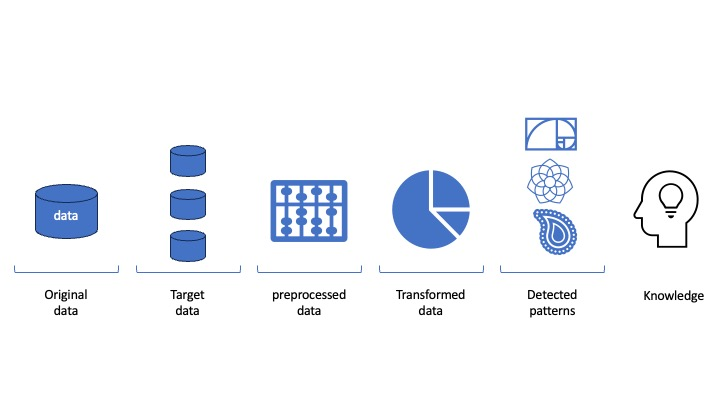
\includegraphics[scale=0.55]{figures/imagens-tese.jpg}

\caption{\ac{kdd} Process, adapted from \cite{Fayyad_Piatetsky-Shapiro_Smyth_1996}} \label{fig:kdd-generic}
\end{figure}

Several frameworks have been proposed to implement the \ac{kdd} process. One such prominent framework is \ac{crispdm}, which comprises business understanding, data understanding, data preparation, modelling, evaluation, and deployment. \ac{crispdm} was conceived in 1996 and became a \ac{eu} project under the ESPRIT funding initiative in 1997 \cite{Chapman2000CRISPDM1S}. %extend 
%Another significant framework is \ac{kddf}, which is designed explicitly for healthcare applications. It focuses on the acquisition and integration of data from diverse healthcare sources, data preprocessing, data mining, data interpretation, and knowledge utilization. %%FAKE
%semma é proprietário

Furthermore, \ac{d3m} 
\cite{huangDataMiningIntegrated2009} and \ac{semma} \cite{rohanizadehProposedDataMining2009} are also important frameworks for applying \ac{kdd} in healthcare, helping align data mining processes with specific healthcare domains and facilitating more accurate and valuable knowledge discovery.

In the context of \ac{kdd} in healthcare, various classes of algorithms can be utilized, each best suited for different kinds of tasks.

Classification Algorithms: These are used to predict categorical class labels. Examples include Decision Trees, Naive Bayes, \ac{svm}, \ac{knn}, and various types of Neural Networks. These are used in disease diagnosis, patient risk prediction, and readmission prediction.

Clustering Algorithms: These are unsupervised methods used to group similar data points together. K-Means, Hierarchical Clustering, DBSCAN, and Self-Organizing Maps (SOM) are common clustering algorithms used in patient segmentation and anomaly detection.

Regression Algorithms: These are used to predict continuous output variables. Examples include Linear Regression, Logistic Regression, and Regression Trees. These algorithms find application in predicting disease progression and healthcare costs.

Association Rule Mining Algorithms: These discover associations or patterns among a set of items in large databases. Apriori and FP-Growth are commonly used algorithms in this class, helping in discovering co-occurring health conditions or drug interactions.

Sequential Pattern Mining Algorithms: These help discover or predict specific sequence of events, which is particularly useful in medical trajectory analysis.

Most recently, more sophisticated architectures and algorithms appeared with neural networks, generative \ac{ai}, reinforcement learning....

%-tipos de algortimos paraa




\subsection{Evidence Based Medicine}
\ac{ebm} is a relatively recent concept in healthcare, which entails integrating the best available research evidence with clinical experience and patient values to make decisions about patient care. The term "evidence-based medicine" was first coined by a team at McMaster University in Canada in the 1980s, but the concept has historical antecedents dating back to at least the 19th century. This was a time when clinical decision-making was mostly based on untested observations and physicians' experience, leading to variability in treatment strategies. The birth of \ac{ebm} marked a pivotal moment in medical history, aiming to standardize patient care and improve outcomes.

The advent of \ac{ebm} was closely tied to the development of clinical epidemiology, the study of disease patterns, causes, and effects in populations. This field, which emerged in the 20th century, focused on statistical and methodological tools to rigorously evaluate treatments. The early proponents of \ac{ebm} aimed to counter anecdotal and unsystematic approaches to clinical decision-making by insisting on rigorous scientific evidence as a basis for decisions. This transitioned medicine from a largely experience-based discipline to scientific, data-driven practice.

The main concept of \ac{ebm} is the hierarchy of evidence, which classifies different types of research studies based on their methodological quality and applicability to patients. At the top of this hierarchy are \acp{rct} and systematic reviews of \acp{rct}, which are considered to provide the most robust evidence. Observational studies, case series, and expert opinions are further down the hierarchy due to their inherent limitations. \ac{ebm} advocates for the application of the highest level of evidence available in clinical decision-making.

However, \ac{ebm} is not just about applying research findings mechanically to patient care. It integrates these findings with the clinician's expertise and the patient's individual circumstances, values, and preferences. This is known as the triad of \ac{ebm}: best available evidence, clinical expertise, and patient values. The concept recognizes that while evidence can guide decisions, it cannot replace the clinical judgment required in individual cases or the need to consider the patient's personal circumstances and preferences. Thus, \ac{ebm} aims to enhance, not replace, the clinician's traditional skills and roles, adding a new dimension to patient care.


\subsection{Health Data Science}
%sacket 
%- graph of evidence based medicine

%- inconvenient truth ai
%Three controversies in health data science
Health Data Science is an interdisciplinary field that applies rigorous methods to transform healthcare data into actionable knowledge for improving health outcomes. It involves the collection, interpretation, and application of vast amounts of biological, clinical, population, and health system data to improve patient care and public health. The advent of electronic health records, genomics, mobile health technologies, and other forms of big data have fueled the growth of this discipline.

In practice, Health Data Science involves the use of statistical and machine learning methods to analyze healthcare data. This data can be patient records, genomic data, demographic data, and more. It includes elements from various disciplines like biostatistics, epidemiology, informatics, and health economics. The ultimate goal is to provide a data-driven foundation for health decision-making for clinicians, health administrators, policymakers, and researchers.

An integral part of Health Data Science is predictive modelling and hypothesis testing. Predictive modelling involves the creation and use of statistical models or machine learning algorithms to predict future outcomes based on historical data. Hypothesis testing, on the other hand, is used to test the validity of a claim or theory about a population based on sample data. These are crucial for health data science as they allow us to make educated guesses about health trends and outcomes.

Importantly, Health Data Science has significant ethical and privacy considerations. Health data is often sensitive and personal, so maintaining privacy and confidentiality is crucial. This requires secure data handling and storage practices, as well as careful consideration of ethical implications when designing studies and algorithms. Health Data Scientists must also be wary of algorithmic bias and must ensure their models do not perpetuate or amplify health disparities. The ultimate goal of Health Data Science is to improve patient outcomes and health equity using the best available data and methods.


The potential of using systematically created data in healthcare, which reaches the PB, has certainly a lot of potential. However, we have seen in the past as well, that the hype of \ac{ai} and \ac{ml} usually is not supported by truth. There are currently six main aspects that hinder the potential of health data science \cite{panchInconvenientTruthAI2019,peekThreeControversiesHealth2018}:
\begin{myitemize}
    \item interoperability
    \item semantic
    \item secondary usage
    \item data quality
    \item privacy and ethical
    \item observational data
\end{myitemize}

\textbf{Interoperability} is defined by .... sos and soo
there are so and so definition
%aulas



has been a key factor in gathering data. With tens or hundreds of different systems in every health institution, the possibility of exchanging data between \acp{ehr} gets a vital role. The usage of interoperable standards is of extreme importance in order to tackle the need of getting data with a predefined structure.


\textbf{Semantic} adds a additional layer of the \\
%mts ehrs
%mts 
\textbf{Secondary usage} is related with the fact that we are aiming to use data for a purpose for whihch the data was not created for. The main goal for the healthcare data is to provide care. It is not meant for analysis and gain insights.\\

\textbf{Data Quality} stems  from the secondary usage. Since it is a very complicated concepts...\\


\textbf{privacy and ethical} adds a additional layer of the \\

%%%LLM
%Health data science and evidence-based medicine are closely intertwined fields that leverage the power of data analysis and research to improve patient outcomes and inform clinical decision-making. Health data science involves the collection, management, and analysis of vast amounts of health-related data, including electronic health records, medical imaging, genomics, and wearable devices. By applying advanced statistical and machine learning techniques to these datasets, health data scientists can uncover patterns, trends, and insights that can enhance our understanding of diseases, treatment effectiveness, and population health.

%Evidence-based medicine, on the other hand, is an approach to clinical practice that integrates the best available research evidence, clinical expertise, and patient values and preferences. It aims to guide healthcare professionals in making informed decisions about patient care by using rigorous scientific evidence. Health data science plays a crucial role in evidence-based medicine by providing the necessary data and analytical tools to generate high-quality evidence. Through the analysis of large-scale health datasets, researchers can identify associations, evaluate treatment effectiveness, and uncover potential risk factors, all of which contribute to the evidence base that informs clinical practice guidelines and treatment recommendations.

The integration of health data science and evidence-based medicine has the potential to revolutionize healthcare delivery and improve patient outcomes. By leveraging the power of data analysis and advanced algorithms, health data scientists can identify novel biomarkers, develop predictive models, and personalize treatment plans based on individual patient characteristics. This not only enhances clinical decision-making but also enables precision medicine, where treatments can be tailored to the specific needs of each patient. Additionally, the use of health data science in evidence-based medicine allows for the continuous monitoring of treatment effectiveness and safety, facilitating the identification of best practices and the refinement of clinical guidelines over time.

In conclusion, health data science and evidence-based medicine are interconnected fields that rely on each other to drive advancements in healthcare. Health data science provides the necessary tools and techniques to analyze large and complex datasets, enabling the generation of high-quality evidence that informs evidence-based medicine. The integration of these disciplines holds immense potential to transform healthcare by enabling personalized medicine, improving patient outcomes, and enhancing clinical decision-making.



\subsection{Artificial Intelligence}
The idea behind the issue is that \ac{ai} is fundamental to leveraging the potential of the data. \ac{ai} has already been under public focus for a few years now, but its concept is still elusive. 
Mainly because the definition has been changing rapidly as well. If in the 90s, the computer program that played chess could be considered \ac{ai} at the time, nowadays is a very simple and common concept to develop. This is connected with the concept that \ac{ai} is tightly connected with the subjective nature of humans. If we feel that \ac{ai} is something related to what a human can do, it can be widely diverse from person to person.
....
however, there are some definitions that could be interesting to explore in order to get the concept for the purpose of this thesis cleared up.

From \cite{DBLP:books/aw/RN2020}

According to the European Commission \cite{DefinitionAIMain2019} and \cite{EthicsGuidelinesTrustworthy2019}

%%what is ai - livro ai verde + european comission
%what is ai - european comission



\subsection{Explainable Artificial Intelligence}
\ac{ai} has experienced unprecedented advancements in the last decade, leading to its integration in various domains, including medicine. It has been instrumental in transforming clinical decision-making, drug discovery, patient monitoring, and predicting disease trajectories. Despite these advancements, the "black box" nature of complex \ac{ai} models poses interpretability challenges, limiting their widespread adoption in healthcare, a field where transparency, reliability, and understanding of decision-making processes are vital. This lack of interpretability, also known as opacity, can lead to misdiagnoses, inappropriate treatment plans, and, most importantly, breaches in trust among clinicians, patients, and \ac{ai} systems.

As such, the concept of \ac{xai}, which aims to create a suite of techniques that produce more explainable models while maintaining a high level of predictive accuracy, has gained significant attention in medical \ac{ai} research. \ac{xai} seeks to bridge the gap between \ac{ai} opacity and human interpretability, and in doing so, it can enhance the transparency, reliability, and acceptance of \ac{ai} applications in the healthcare setting.

So, for this to happen, we need a new framework for applying such mechanisms. A new step that could be attached to the ones seen before in section \ref{sec:kdd} will enable human comprehension of the model's output.

Even though several grouping and taxonomies of \ac{xai} are available mentioned in \cite{adadiPeekingBlackBoxSurvey2018,linardatosExplainableAIReview2020,barredoarrietaExplainableArtificialIntelligence2020,linardatosExplainableAIReview2020,kamath2021explainable}, a simplified approach based on \cite{kamath2021explainable} will be used in order to contextualize this concept.

We can divide it into two main categories. Firstly the explanation type, which is divided into global and local. Local and global explanations are methods used to interpret machine learning models, especially those that are considered "black box" models, such as deep learning networks. These methods help us understand why and how a model makes certain decisions, which can be crucial in many settings for ethical, legal, and practical reasons.

Local Explanations: These involve understanding the prediction of a \ac{ml} model for a specific individual instance. They help to answer questions like: "Why did the model predict that this particular patient has cancer?" or "Why was this specific transaction flagged as fraudulent?". 

Global Explanations: These focus on understanding the model behaviour across all instances, or more broadly on a dataset-wide level. They help to answer questions like: "What features are generally important for prediction in the model?" or "What is the overall logic of the model?". 

Secondly, we have the method type, where we have 3 main subcategories related to the stage of the data science process it is applied, pre, during and post-model training.

\textbf{Pre-Model \ac{xai}:} These methods involve improving the transparency and interpretability of models before they are even trained. This includes thoughtful feature engineering, \ac{eda}, and applying domain knowledge to create meaningful variables. The goal is to design a model that will be more interpretable from the onset.

\textbf{Intrinsic \ac{xai}:} This involves using machine learning models that are intrinsically explainable. These models are designed in such a way that their decision-making process is understandable by default. Examples include linear and logistic regression, cox regressions, decision trees, Naïve Bayes, \ac{bn} and rule-based models. While these models may sometimes lack the predictive power of more complex models, they provide clear interpretability: you can directly examine the impact of the variables and understand how the model makes its predictions.
\\
\textbf{Linear Regression}
Linear regression is a linear approach to modeling the relationship between a dependent variable and one or more independent variables. It assumes that the relationship between these variables is linear and can be represented by a straight line. The goal is to fit the best possible line that describes this relationship by minimizing the sum of the squared differences (errors) between the observed values and the values predicted by the line. Linear regression is widely used in various fields for prediction, modeling, and determining the strength and character of the relationship between variables. It forms the basis of many more complex statistical modeling techniques.
\\
\textbf{Logistic Regression}
Logistic regression is used to model the probability of a binary outcome that depends on one or more independent variables. Unlike linear regression, which predicts a continuous outcome, logistic regression predicts the probability of a categorical outcome (e.g., success/failure, yes/no, 1/0). The logistic function is applied to the linear combination of independent variables to ensure that the estimated probabilities are between 0 and 1. It's often used in fields like medicine, economics, and social sciences to predict the likelihood of an event occurring based on various factors.
\\
\textbf{Cox Regression}
Cox regression, or the Cox proportional-hazards model, is a statistical technique used for investigating the effect of several variables on the time a specified event takes to happen. In medical research, this often refers to survival times. The model allows for the estimation of hazard ratios, which describe how the hazard changes with a one-unit change in the predictor variable. The Cox model makes an assumption that the hazard ratios are constant over time, known as the proportional hazards assumption. This model is vital for understanding how different factors influence survival or failure time and is commonly applied in epidemiological and medical research.

\textbf{Bayesian Networks}
A \ac{bn}, also known as a belief network or \ac{dag} model, is a probabilistic graphical model that represents a set of random variables and their conditional dependencies via a \ac{dag}. 

Given a set of variables \(X = \{X_1, X_2, ..., X_n\}\), the joint probability distribution is given by:

\[
P(X_1, X_2, ..., X_n) = \prod_{i=1}^{n} P(X_i | Parents(X_i))
\]

where \(Parents(X_i)\) is the set of parent variables of \(X_i\) in the network.

This formula represents the factorization of the joint distribution over \(X\), based on the graphical structure of the Bayesian network.

Now, in the Bayesian network, each node is conditional independent of its non-descendants given its parents. If we denote \(ND(X_i)\) as the set of non-descendants of \(X_i\) and \(Pa(X_i)\) as the parents of \(X_i\), the conditional independence is described as:

\[
X_i \perp ND(X_i) | Pa(X_i)
\]

This means that \(X_i\) is conditionally independent of its non-descendants given its parents. 

A common task for Bayesian networks is inference, which means computing the posterior probability of a set of query variables \(Q\), given some observed variables \(E\). That is, we want to compute \(P(Q|E)\). According to the Bayes rule, we have:

\[
P(Q|E) = \frac{P(Q,E)}{P(E)} = \frac{P(Q,E)}{\sum_{q \in Q} P(Q=q,E)}
\]

where the denominator is a normalization constant ensuring the result is a valid probability distribution. Note that performing this inference is NP-hard, which is why various approximation algorithms have been developed.

\textbf{Tree based methods}
Tree-based machine learning methods are a subset of algorithms that use a tree-like graph structure for making decisions or predictions. The most basic type is the Decision Tree, where the tree is used to go from observations about an item to conclusions about the item's target value (classification or regression). Each node in the tree represents a feature in the dataset, each branch represents a decision rule, and each leaf node represents the output value. More advanced tree-based methods include Random Forests, which build multiple Decision Trees and average their predictions for better accuracy and generalization, and Gradient Boosted Trees, which build trees sequentially, each one correcting the errors from the previous one.

The major advantage of tree-based methods is their ease of interpretation and understanding, especially for Decision Trees. However, a single tree is often prone to overfitting, where it performs well on the training data but poorly on unseen data. This is why ensemble methods like Random Forest and Gradient Boosting are popular; they aim to increase robustness and predictive power by combining multiple trees. These methods are widely used in various domains including but not limited to finance, healthcare, and natural language processing for tasks like classification, regression, and even unsupervised learning tasks like clustering.

\textbf{Post-Hoc \ac{xai}:} Post-hoc methods are applied after a model has been trained, to try to explain its decisions. This includes techniques like feature importance analysis, partial dependence plots, \ac{lime}, \ac{shap} and counterfactuals. For instance, \ac{lime} can be used to create local explanations for individual predictions made by any model, and \ac{shap} values can be used to interpret the impact of features on the model's output both locally and globally. Counterfactuals try to explain a model by example, providing possible changes that would alter the outcome provided by the model.

It is to be noted that a methodology can be classified into two categories. For example, \ac{lime} is a local explanation model in a \textit{post-hoc} manner.

Finally, we can assess how these three types of model are in fact an explanation of the model, we could argue, like stated in \cite{rudinStopExplainingBlack2019} that only an intrinsically transparent model can really be the basis of \ac{xai} and applying \textit{post-hoc} methods is only a potentially wrong proxy for an explanation.
%explicar mais disto e fechar.

\subsection{Causality}

In order to merge the \ac{ebm} and \ac{xai}, we can follow on to the realm of \ac{cml}.

%- causality vs observation

\ac{cml} is a branch of machine learning that focuses on understanding and quantifying causal relationships from data. Instead of just finding patterns or correlations in data, \ac{cml} aims to uncover the cause-and-effect relationships that explain these patterns.
This is specially important since current or traditional \ac{ml} and \ac{ai} methodologies rely heavily in association and not causation. So, \ac{cml} can support traditional algorithms to solve its limitations \cite{pearlTheoreticalImpedimentsMachine2018}.
There are currently two main frameworks for trying to unveil causality in data: the \ac{scm}  and the \ac{pof} \cite{shiLearningCausalEffects2022b}.

\ac{scm} relies on \acp{dag} and structual equations.
Causal Graphs are based on \acp{dag}: These are graphical models used to represent causal relationships between different variables. The nodes in the graph represent variables, and the edges (arrows) between nodes represent causal relationships. For instance, an edge from Node A to Node B signifies that A has a causal effect on B. We should not confuse causal graphs with \ac{bn}. Even though both rely on \acp{dag}, Causal Graphs represent causal relationships, and \ac{bn} represent conditional dependencies.
%% SCM???
strucurual equations....


The \ac{pof} model centers on the concept of potential outcomes which can be understood as all of the possible outcomes for a patient.  Each unit (e.g., a patient or a sample) has a set of potential outcomes, each corresponding to one of the possible treatments the unit could receive. The causal effect is defined as the difference between these potential outcomes. This framework allows for the formal definition and estimation of causal effects. In this approach, we consider the potential outcomes for each unit (for example, a patient in a healthcare context) under each possible treatment or intervention. Each unit has a set of potential outcomes corresponding to each possible intervention. However, we can only observe one of these outcomes for each unit, corresponding to the intervention that was actually received. The other outcomes, which would have occurred had different interventions been implemented, remain latent. These are known as counterfactual outcomes.

The difference between potential outcomes under different treatments represents the causal effect of the treatments. For instance, in a healthcare scenario, if we are studying the effect of a drug, we might consider two potential outcomes for each patient: the outcome if the patient is given the drug, and the outcome if the patient is not given the drug. The difference between these outcomes represents the causal effect of the drug on the patient. However, as we can only observe one of these outcomes for each patient (the one corresponding to the treatment they actually received), a key challenge in causal inference is estimating the unobserved potential outcomes. Various statistical methods, including randomized experiments, matching methods, and instrumental variable methods, can be used to estimate these unobserved potential outcomes.


Counterfactuals: This is a concept rooted in the idea of "what-if" scenarios. A counterfactual outcome for a given individual is the outcome that would have occurred had the individual been exposed to a different treatment or condition.
%%

Counterfactuals play a pivotal role in the field of causal machine learning, offering a sophisticated approach to understanding cause-and-effect relationships. In essence, a counterfactual is a conceptual device used to contemplate what would have happened under a different set of circumstances than what actually occurred. This hypothetical scenario is created by altering some aspect of the actual situation, providing a means of comparison to evaluate the effect of a particular variable or intervention.

For instance, in the context of healthcare, consider a scenario where a patient was given a particular drug and recovered. The counterfactual question here would be: "What would have happened to the patient if they hadn't been given the drug?" Answering this question allows us to estimate the causal effect of the drug on the patient's recovery. While the true counterfactual outcome is unobservable (since we cannot rewind time and alter the decision), various statistical techniques, machine learning algorithms, and experimental designs are employed in causal inference to estimate this effect as accurately as possible. The ability to make such counterfactual inferences is crucial in numerous fields, including medicine, economics, social sciences, and policy-making, where understanding causal relationships is paramount.


%Confounding Variables: These are variables that both affect the treatment assignment and the outcome. Confounding variables can create spurious associations that can be mistaken for causal relationships, so they must be carefully controlled for in causal analyses.
%%%
%Confounding variables, also known as confounders, represent a major challenge in the study of causal relationships. A confounding variable is a variable that influences both the dependent variable and independent variable, causing a spurious association. This can lead to false conclusions about the relationship between the independent and dependent variables, obscuring the true causal effect.

%For instance, imagine a study investigating the relationship between physical exercise (independent variable) and health outcomes (dependent variable). Age could act as a confounding variable in this scenario. Older individuals might exercise less than younger ones, and they also tend to have more health problems. Without proper adjustment, the study might falsely attribute the poorer health outcomes solely to a lack of exercise, while in reality, age is influencing both exercise habits and health outcomes.

%Confounding variables can be addressed in a number of ways. In the design stage of a study, randomized controlled trials (RCTs) are used to ensure that confounding variables are evenly distributed across treatment and control groups, thereby reducing their impact. In observational studies where random assignment is not possible, statistical techniques such as regression adjustment, stratification, matching, and propensity score methods can be employed to control for confounding. Importantly, the success of these methods depends on the ability to measure all relevant confounders, a challenge known as unobserved confounding, which is a persistent issue in causal inference.



Instrumental Variables: These are variables that are related to the treatment but not the outcome, except through their effect on the treatment. They can be used to control for unmeasured confounding variables.
%%%%

Instrumental variables (IVs) are a powerful tool used in causal inference to help address the problem of confounding variables, especially in situations where randomization is not feasible. An instrumental variable is a variable that is correlated with the independent variable (the treatment) but does not directly affect the dependent variable (the outcome), except through its effect on the treatment. In other words, it is a variable that induces changes in the explanatory variable but is otherwise unrelated to the outcome of interest.

The idea behind using an instrumental variable is to isolate the portion of the variation in the treatment that is independent of the confounders, and therefore provides a "natural" form of randomization. The causal effect of the treatment on the outcome can then be estimated based on this variation.

For example, in a study assessing the impact of education on income, it's challenging to identify causal effects because numerous unobserved factors (like ability or motivation) could affect both education and income, thus confounding the relationship. If we find an instrumental variable – say, distance to the nearest college (which affects the likelihood of getting higher education but doesn't directly affect income) – we can use this to isolate the part of the variation in education that is unrelated to the unobserved confounders, and thereby get a more accurate estimate of the causal effect of education on income.

It's crucial, however, to remember that the use of instrumental variables relies on certain assumptions, such as the relevance and exogeneity of the IV. The relevance assumption requires that the IV is correlated with the treatment, and the exogeneity assumption requires that the IV affects the outcome only through the treatment and is not related to the unobserved confounders. Violations of these assumptions can lead to biased and inconsistent estimates of causal effects.



Propensity Score: This is the probability of a unit (e.g., a patient) being assigned to a particular treatment given a set of observed characteristics. Propensity scores are used to balance the characteristics of treatment and control groups, mimicking the conditions of a randomized experiment.
%%%%

The propensity score is a statistical concept widely used in causal inference, particularly in the field of observational studies where random assignment of treatment is not possible. The propensity score for an individual is the probability of receiving the treatment given the observed characteristics of that individual. In other words, it's the likelihood that a particular individual would be assigned to the treatment group based on their observed features.

The key idea behind propensity scores is to create a balance between the treatment and control groups based on these observed characteristics, thus mimicking the conditions of a randomized controlled trial. This balance helps to eliminate bias caused by confounding variables, allowing for a more accurate estimate of the treatment effect. Once propensity scores are calculated, they can be used in several ways including matching, stratification, inverse probability of treatment weighting (IPTW), and as covariates in regression adjustment.

For example, consider a study investigating the effect of a training program on job outcomes. Individuals might self-select into the training program based on characteristics like motivation or prior education, which are also related to job outcomes, creating confounding. The propensity score, calculated based on these observed characteristics, can be used to match each participant in the training program with a similar non-participant or to weight the observations, such that the distribution of observed characteristics is similar between the groups. This helps to isolate the effect of the training program on job outcomes.

However, it's important to note that propensity scores only account for observed confounders. If there are unobserved confounders that influence both treatment assignment and the outcome, propensity score methods may still produce biased estimates of the causal effect.



%These concepts and others are used in methods like matching, instrumental variable analysis, difference in differences, regression discontinuity, and others to estimate causal effects. The goal of all these techniques is to create a situation as close to a randomized control trial as possible, as this type of experiment is considered the "gold standard" for estimating causal effects.



\subsection{All of this brought together}

So....



\section{Legal and ethical considerations}

%GDPR, health european data space, questoes eticas


As data science and \ac{kdd} become increasingly prevalent in the healthcare sector, the legal and ethical considerations related to these practices also become critically important. Ensuring the proper use of healthcare data is key to preserving public trust and ensuring the long-term viability of data-driven health initiatives.

One of the primary legal considerations is data privacy. Laws such as the \ac{hipaa} in the \ac{us}, and the \ac{gdpr} in the \ac{eu}, set stringent rules on how healthcare data should be stored, shared, and processed. They require data scientists and healthcare providers to take steps to anonymize data and limit the scope of data usage. Breaching these regulations can lead to severe penalties, including fines and imprisonment.

On the ethical front, considerations include ensuring data fairness and avoiding bias. Given the diversity of patients in terms of age, race, sex, socioeconomic status, etc., algorithms should be designed and validated to ensure that they don't unintentionally perpetuate or amplify societal biases. For instance, a predictive model for disease risk should not unfairly disadvantage certain demographic groups. Furthermore, the informed consent of patients is another significant ethical consideration. Patients should be fully informed about how their data will be used, and they should have the right to opt-out if they wish.

Transparency is another crucial aspect that straddles both legal and ethical dimensions. It involves explaining how decisions or predictions are made by complex algorithms, particularly when they have significant implications for patient care. For instance, if an AI model is used to prioritize patients for treatment, it should be transparent about how the model makes its decisions. The explainability of machine learning models can help achieve this transparency, which aids in maintaining accountability and trust.

Lastly, there's the matter of data security. With the rise of cyber-attacks, ensuring the robustness of the system against such breaches is both a legal requirement and an ethical obligation. Security breaches could lead to sensitive patient data being stolen, with severe implications for the individuals involved and for the trust in the healthcare system as a whole.

%In conclusion, while data science and KDD offer immense potential to improve healthcare, it is crucial that these technologies are implemented in a way that respects legal regulations and ethical principles. This will help to ensure the sustainability and public acceptance of these technologies in the long run.

In a parallel layer to this one, we have ethical issues. If we use data to derive knowledge and create  \acp{cdss} that orient and support clinical practice, they can be biased by the type of data that originated said knowledge.
This could lead to biased and discriminatory systems....

%%%chat
The importance of ethics in \ac{ai} cannot be overstated, primarily because the decisions that these systems make can have profound implications on individuals and society. These decisions may affect anything from employment opportunities to legal outcomes, and increasingly, health outcomes. As AI models grow in complexity and application, they possess an enormous power that needs to be harnessed responsibly. This necessitates rigorous ethical considerations to ensure fair, unbiased, and transparent operations. Ethical lapses can result in discrimination, loss of privacy, and unjust outcomes, among other issues, which erode public trust in these technologies.

Equally important in the realm of AI is the understanding of why a model works the way it does. This concept, known as "explainability" or "interpretability", is central to AI ethics. It concerns the transparency of AI algorithms and the ability to understand and interpret their inner workings and decisions. Without this understanding, we run the risk of blind reliance on AI's 'black box' that may lead to erroneous or biased outcomes. It is critical to scrutinize AI models' reasoning processes, ensuring they align with human values and principles and are not based on inappropriate or discriminatory features.

In the context of healthcare, these considerations take on an even greater significance. AI applications in healthcare, such as diagnostic tools or treatment recommendation systems, directly impact human lives. They may influence critical decisions such as who gets treatment, what kind of treatment is administered, and when it should be given. These systems must not only be accurate but also transparent, fair, and accountable. They should be designed and implemented in a way that respects patient rights, including privacy, autonomy, and informed consent.

Therefore, in healthcare, the need for ethical AI and model explainability is not just a matter of good practice, it's a matter of life and death. Bias or errors in AI could lead to misdiagnoses or inappropriate treatment recommendations, with potentially fatal consequences. Similarly, if AI-based systems make decisions that healthcare professionals or patients can't understand, it may lead to mistrust and potential harm. It's crucial for the advancement of AI in healthcare to ensure ethical considerations and explainability are at the core of AI model design, development, and deployment. This will build trust in AI systems and ultimately lead to better health outcomes.
\begin{savequote}[85mm]
    Nothing travels faster than the speed of light, 
    with the possible exception of bad news, which obeys its own special laws.
    \qauthor{Douglas Adams}
    \end{savequote}


\chapter{Research Methods to Improve Data Quality}\label{chap:goal1}
This chapter focuses on enhancing data quality through innovative research methods. Firstly, the utilization of synthetic data generation, as detailed in sections \ref{subsec:gans}, \ref{subsec:tabular}, and \ref{subsec:similarity}, serves a dual purpose: expanding the volume of available data while simultaneously safeguarding privacy. This approach focuses on  techniques such as \acp{gan} to create realistic, yet non-sensitive data sets. Secondly, the development of automatic data quality assessment methods, explored in section \ref{subsec:dq}, marks a significant stride in ensuring the integrity and reliability of data. These methods aim to automate the process of evaluating data quality, thus reducing manual effort and increasing the efficiency and accuracy of data analysis.



\section{Can GANs Help Create Realistic Datasets?}\label{subsec:gans}
This section is based on the paper entitled "GANs for Tabular Healthcare Data Generation: A Review on Utility and Privacy". It focuses on a review of the \ac{gan} framework for creating synthetic data for healthcare. Tries to compile the metrics used for comparing and assessing synthetic data in terms of utility - or how similar they are to the original data and privacy - how protective of the patient's data it is. 

% !TeX root = ../thesis.tex

\subsection{Introduction}

With the growing technological advances, the quantity of healthcare-related data produced around the world increased exponentially \cite{choi_generating_2017,henry_adoption_2016}.
Consequently, the potential for harvesting this data also increases. The value locked within
this data could help provide better healthcare with new information about diseases,
drugs, and preventive therapies. It can also help create better \acp{his}, meaning an overall better clinical practice \cite{ISI:000502534100049}. But for this to happen, data must reach capable hands at the right time.
But the release of clinical data has several barriers attached and rightly so. The leakage of patient’s privacy can break the confidence of the population in healthcare
professionals and institutions. Patient safety
and privacy should be kept at all costs. However, the current mechanisms for privacy maintenance are very long, bureaucratic, and time-consuming, nationally \cite{comissao_nacional_protecao_de_dados_principios_2015}, and internationally \cite{office_for_civil_rights_guidance_2013}. The current scenario and general methods for privacy safeguards are related to pseudo-anonymisation techniques.
The removal of certain attributes, identifier modification, code grouping, or discretization are some methodologies. But not even these are totally safe \cite{el_emam_systematic_2011}.
Synthetic data appear as an alternative for clinical data sharing, promising great data
utility with minimal privacy concerns. Synthetic data is data that is generated automatically through programmatic processes. This is especially impactful for the case at hand
since synthetic data has no explicit connection with the original data. There are several
mechanisms for data synthesis postulated by \cite{goncalves_generation_2020}, there are
process-driven methods and data-driven methods. Process-driven methods generate
data through pre-determined models inputted into the generator. Data-driven methods
produce new data based on inputted source data. With this, it is possible to create new
patient data that has no relation to reality while providing the same statistical relations
between variables. This provides the basis for quality clinical research on top of this
new data. Even though these techniques are still new and in rapid development, the
results seem interesting \cite{goncalves_generation_2020}, but not without questions and doubts
\cite{stadler_synthetic_2020}.
Creating a thorough survey based on the generation of synthetic data is seldom a simple task when compared to other surveys since synthetic data is present across several domains and has several uses, like software testing, assessing methods, or generating hypotheses. Moreover, synthesis has
the double meaning of summing up information and generating something, easily wielding hundreds of results per query. Finally, trying to filter
algorithms aimed at tabular data is also burdensome, since not always it is easy to discriminate input types. These factors make the survey interesting to focus on the state-of-the-art mechanisms of generating tabular data.

\subsection{Theoretical background}
First introduced in 2014, \acp{gan} \cite{goodfellow_generative_2014} have been under the scope and have been proven very good for generating complex data. Images, text, and video have been successfully generated with very good performances. %cite?
The original architecture is based on two artificial neural networks trained simultaneously in a competitive manner. One of them, the generator, has the objective of generating the most realistic possible data, while the second network – the discriminator, has the opposite aim of aiming to distinguish the realistic data from the synthetic
data the best it can. So, the elegance of this architecture is that each network tries to
make the other perform better every time. The \ac{gan} architecture is shown in \ref{fig:gan-arch}.
% w - \omega
% θ - \theta
% G - generator
% D - discriminator

\begin{figure}
\centering
%\includegraphics[width=\textwidth]{image.png}
\includegraphics[scale=0.75]{figures/image.png}

\caption{\ac{gan} framework} \label{fig:gan-arch}
\end{figure}
The generator is represented by $G_{\theta}$ where the parameter $\theta$ represents the weights of
the neural network. It takes as input, a Gaussian random variable, and outputs $G_{\theta}$(Z).
Distribution of $G_{\theta}$(Z) is denoted by $P_{\theta}$. The goal of the generator is to choose $\theta$ such that the output $G_{\theta}$(Z) has a distribution close to the real data. The discriminator is represented by $D_{\omega}$, parametrized by weights $\omega$. The goal of the discriminator is to assign 1 to the samples from the real distribution $P_{X}$ and 0 to the generated samples ($P_{\theta}$). So, \acp{gan} can be mathematically represented by a \textit{MinMax} game identified by:
\begin{equation}
\min_{G}\max_{D} \; E [log(D_{\omega}(X)) + log(1-D_{\omega}(G_{\theta}(Z))]
\end{equation}
So, $G$ must minimize this equation and $D$ must maximize it, each one tweaking the weights of its network ($\theta$ and $\omega$) to do so. This is the loss function on the initial \ac{gan} architecture. After the classification of $D$, the $G$ is trained again with the error signal from $D$ through backpropagation. This equation is the log of the probability of $D$ predicting that the real data is genuine and the log probability of $D$ classifying synthetic data as not genuine. The equation is essentially the same as minimising the \ac{jsd} \cite{goodfellow_generative_2014}:
\begin{equation}
\min_{G} JS(P_{x}||P_{\theta})
\end{equation}
Where the JS means the \acl{jsd} between the probability of the real data and the probability of the generated data. The JS divergence provides a measure of the distance between two probability distributions. Therefore, the minimization over $\theta$ means, choosing the $P_{\theta}$ that is closest to the target distribution $P_{X}$ in the JS divergence distance. Despite the significant results provided by \acp{gan} with continuous real values, categorical values still seem to be a problem for this approach \cite{kusner_gans_2016}, since it is not directly applicable for calculating the gradients of latent categorical variables in order to train these networks through backpropagation. This happens since the output of the generator, even though can be transformed into a multinomial distribution with a \textit{softmax} layer, sampling from it is not a differentiable operation, limiting the backpropagation process of the \ac{gan}.

%One of the most famous alternative GAN architectures is the \textit{Wasserstein}  GAN (WGAN)
%\cite{arjovsky_wasserstein_2017} . It improves GAN by using the \textit{Wasserstein} distance instead of the \textit{Jensen-shannon divergence}. It is represented by the
%following minimax game:
%\begin{equation}
%\min_{G}\max_{\omega \; \epsilon \;W} \;\; E[f_{\omega}(X)] - E[f_{\omega}(G_{\theta}(Z))] 
%\end{equation} 
%Where functions $f_{\omega} \;  \omega \; \epsilon \;W$  are all \textit{K-Lipschitz} (with respect to $x$) for some K.
%This was proposed because it helps prevent mode collapse, where the generator maps
%several inputs to the same output. An example of this is a generator that starts creating
%several images with the same patterns or colours. The fact that this loss function can be
%very customisable in distinct GAN implementation, applying different functions can
%lead to different outcomes and architectures.

%\iffalse
%\subsubsubsection{Differential privacy}
%The privacy model most used in generative models is differential privacy \cite{dwork_differential_2006}. It is a mathematical model for measuring privacy loss. The basis of it is a mechanism that adds noise to a dataset through randomisation. Applying differential privacy is a method for guaranteeing that adding or removing any record from the original data does not influence the generation output. The formal definition, as stated in \cite{dwork_differential_2006} is:
%\begin{equation}
%Pr[M(x)\; \epsilon \; S] \leq e^\varepsilon Pr[M(y)\; \epsilon \; S] + \delta
%\end{equation} 
%Where M is a randomised mechanism, $\varepsilon$ is the privacy budget (balance between privacy and utility). The $x$ and $y$ represent adjacent datasets that differ on only one record. So, we say that M gives $\varepsilon$-differential privacy if the probability of seeing an event S in the $x$ dataset is at most equal to $e^\varepsilon$ multiplied by the probability that we see S when the dataset is $y$. Variable $\delta$ is the probability of an uncontrolled breach. With this, a smaller $\varepsilon$ will yield better privacy but a less accurate response, so it can be used to tweak the utility and privacy of the dataset.
%\fi

\subsection{Methods}
This search was made between December 2020 and January 2021. It was made on “Web of Science”, IEEE, PubMed, Arxiv and finally GitHub. The terms searched were related to \acp{gan}, synthetic data generation, electronic health records, patient data, or tabular data. Applications of \acp{gan} to non-tabular data were filtered, like image, sound, video, or graphs. Time series and text data were also removed since the methodology for synthesizing this type of data has specific functions related to the nature of the data. The filter for date was after 2014 since \acp{gan} were introduced at that time. The queries used were similar to the one below, adapted for the search mechanics for each website.


\begin{scriptsize}

{\fontfamily{courier}\selectfont
("generation" OR "creation" OR "synthesis" OR "synthesizing" OR "generating" OR "creating") AND ("synthetic data" OR "synthetic patient" OR "synthetic electronic health record" OR "synthetic EHR" OR "realistic patient data" OR "realistic health record" OR ("synthetic" AND "privacy" AND "utility"))  AND ("GAN" OR "Generative Adversarial Network")}
\end{scriptsize}
%\begin{verbnobox}[\scriptsize]
%("generation" OR "creation" OR "synthesis" OR "synthesizing" OR
%"generating" OR "creating") AND ("synthetic data" OR
%"synthetic patient" OR "synthetic electronic health record" 
%OR "synthetic EHR" OR "realistic patient data" OR "realistic 
%health record" OR ("synthetic" AND "privacy"  AND "utility")) 
%AND ("GAN" OR "Generative Adversarial Network")
%\end{verbnobox}

From the total articles found (1165) with all the queries, 100 articles were chosen for full text and in the end, 22 papers with \ac{gan} implementations that were tested on tabular data were selected. 
%These implementations were studied and evaluated in terms of privacy concerns and utility performance and compared when possible. 
%For selecting the articles and helping with paper selection, RAYYAN QCRI online \cite{rayyan:14:cochrane} was used along with Mendeley Reference Manager for paper management.


\subsection{Results}
The selected papers ranged from 2017 to 2020. Being that 2 are from 2017, 4 from 2018, 8 from 2019 and 8 from 2020. All authors showed original \ac{gan} implementations, apart from 2 papers. Beaulieu-Jones et al. \cite{beaulieu-jones_privacy-preserving_2019} used a
\ac{gan} architecture that was originally published with usage on image datasets \cite{odena_conditional_2017}. Additionally, Vega-Marquez et al.  \cite{ISI:000490706700022} used an already known implementation of conditional \acp{gan} \cite{mirza_conditional_2014}. We classified papers regarding 3 metrics: utility, privacy and clinical. For utility, we looked for  methods for measuring the generated data's quality. As for privacy, we aimed for some mechanism for measuring the privacy loss of the new data. Concerning clinical metrics, any kind of evaluation from healthcare professionals was considered. This can be seen in table \ref{tab:review_gans}.


\begin{table}[tphb]
\caption{Summary of the articles selected. The year, acronym, reference and  type of metrics mentioned are indicated. Code repository is mentioned when such information was provided. }\label{tab:review_gans}
\centering
\small
\begin{tabular}{lllclc}
%\begin{tabular}{l|llclc}

\toprule
 ID & year  & Acronym & Article & Metric & Code \\

% & \multicolumn{1}{|c}{Year \hspace{2 mm}}  & \multicolumn{1}{|c|}{Acronym} & \multicolumn{1}{c}{\hspace{2 mm} Article \hspace{1 mm}} & \multicolumn{1}{|c|}{Metric} & \multicolumn{1}{c|}{\hspace{2 mm}Code \hspace{2 mm}}  \\

\midrule
1 & 2017 & medGAN  &\cite{choi_generating_2017}          & Utility, Privacy, Clinical \hspace{1 mm} &  \cite{medGANurl}  \\

2 & 2017 & POSTER & \cite{ISI:000440307700174} & Utility, Privacy  &   \cite{POSTERurl}\\

3 & 2018 & table-GAN & \cite{park_data_2018} & Utility, Privacy         &   \cite{table-GAN-url} \\

4 & 2018 & dp-GAN & \cite{xie_differentially_2018}& Utility, Privacy &   \cite{dp-GAN-url}  \\

5 & 2018 & mc-medGAN & \begin{tabular}[c]{@{}l@{}}\cite{camino_generating_2018}\end{tabular}    & Utility &   \cite{mcmedgan-url}\\

6 & 2018 & TGAN &  \cite{xu_synthesizing_2018}& Utility &  \cite{tgan-url}\\

7 & 2019 & PATE-GAN & \begin{tabular}[c]{@{}l@{}}\cite{jordon_pate-gan_2019}\end{tabular}    & Utility, Privacy   & --\\

8 & 2019 & SPRINT-GAN & \cite{beaulieu-jones_privacy-preserving_2019}           & Utility, Privacy, Clinical &  \cite{sprint-GAN-url} \\

9 & 2019 & GAN-based &     \cite{ISI:000524576200016} & Utility, Privacy & --\\

10 & 2019 & CTGAN &  \cite{xu_modeling_2019} & Utility & \cite{CTGAN-url}\\

11 & 2019 & WGAN-DP & \begin{tabular}[c]{@{}l@{}}\cite{brenninkmeijer_generation_2019}\end{tabular} & Utility, Privacy    & \cite{WGAN-DP-url} \\

12 & 2019 & PPGAN &  \cite{liu_ppgan_2019} & Utility, Privacy &  \cite{ppgan-url}\\

13 & 2019 & medBGAN &   \cite{ISI:000502534100049} & Utility & --\\

14 & 2019 & medWGAN& \cite{medwgan}& Utility &  \cite{medWGAN-url}  \\

15 & 2020 & ADS-GAN& \begin{tabular}[c]{@{}l@{}}\cite{ISI:000557358500024}\end{tabular} & Utility, Privacy& --\\

16 & 2020 & corGAN & \cite{2001.09346}& Utility, Privacy &  \cite{corGAN-url}\\
17 & 2020 & CGAN &  \cite{ISI:000490706700022}& Utility& --\\

18 & 2020 & DPAutoGAN&  \cite{tantipongpipat2020differentially}& Utility, Privacy & \cite{DPAutoGAN-url}\\

19 & 2020 & GAN Boosting& \cite{2007.11934} & Utility, Privacy &  \cite{postganurl}\\

20 & 2020 & RDP-CGAN&  \cite{rdp-gan}& Utility, Privacy &  \cite{rdp-cgan-url}\\

21 & 2020 & WCGAN-GP&  \cite{WCGAN-GP}& Utility, Privacy & --\\
22 & 2020 & SMOOTH-GAN &  \cite{smooth-gan} & Utility & \cite{smooth-gan-url}\\
\bottomrule
\end{tabular}
\end{table}


The metrics the authors used are exhibited in table \ref{tab:results_review}. Regarding privacy, 15 papers assessed it or included some kind of mechanism to improve data protection. The most common was including Differential Privacy (DP) in the generation process. Other mechanisms for measuring privacy loss were Membership Inference (Member. Inf.), Attributes Disclosure (Attrib. Disc.), Euclidean distance (Eucl.), record-linkage (R. Linkage) and \acf{knn}.
As for utility, all papers assessed it. There were 3 major areas of utility assessment: Dimension-wise (DW) probability, cross-testing, and distance metrics. The most basic one was dimension-wise probability, which is important for making sanity checks for the generated data, comparing the distributions of each column between real and synthetic. In this category, we can find \textit{Bernoulli} (Bern.), cumulative distributions (Cumul. Dist.), \textit{Pearson} correlation (Pearson) and \textit{Spearman} correlation (Spearman), correlation coefficients (CCS), chi-squared test ($\chi^{2}$),  \acf{ks} or Correlation Matrices (Corre. Mat.).
Cross-testing was about training machine-learning algorithms with both datasets in order to compare the results. The key factor is generating a synthetic dataset based on the training set and then training models on the original training set and the generated dataset. Then the models are compared regarding their predictive capability on the (real) test set. This was a way of assessing if the generator models were capturing inter-variable relationships. The authors applied different metrics from \acf{auroc}, F1, \ac{auprc}, Accuracy (Acc.) to \acf{mre}. Finally, there was also the application of distance metrics, for measuring the difference between column distribution in both datasets. \acf{jsd}, \textit{Wasserstein} Distance (WD), \textit{Bhattacharyya} Distance (BD) or Generate Scores (GS) that was a metric implemented by the authors of \cite{liu_ppgan_2019} that creates a metric based on the sum of the mean of \textit{kullblack-leibler}  distance of all columns. Other less used methods were \acf{pca}, propensity score mean squared error ratio (pMSE). Normalised Mutual Information (NMI), which is the ability to capture correlations between columns by computing the pairwise mutual information and MMD (Maximum Mean Discrepancy), which is similar to distance metrics were also used. Regarding datasets utilized, the most used was MIMIC-III \cite{mimiciii} (9 times). The papers used 27 different datasets, being 16 healthcare-related and 11 non-healthcare related. 
Finally, regarding clinical evaluation, only two papers assessed it, as it is possible to see in table \ref{tab:review_gans}. Both had a group of clinicians assessing a sample of both real and synthetic information and evaluating from 0 to 10, where 10 is the most realistic.
One major point preventing a larger comparison is that despite some papers using the same dataset and same methodologies, the presented values are different, making it difficult for a clear comparison of results. One example is a dimension-wise prediction with F1 score for MIMIC-III. CorGAN presents the mean difference between the two classifications (real on real and synthetic on synthetic), while medBGAN presents the correlation coefficients of the two, and medGAN only presents the visual comparisons. Regarding code availability, 16 papers had the code publicly available in some form. As of January 2021, papers pointed in table \ref{tab:review_gans} have public code.



\begin{landscape}
\renewcommand{\arraystretch}{1.02} %add more space between cells (1.2 is a factor)
\begin{table}[htbp]
\caption{Summary of different metrics utilised for evaluating synthetic data. Grouped by utility and privacy metrics. Acronyms indicate the source paper} \label{tab:results_review} 

\begin{tabular}{p{26mm} p{84mm} p{60mm}}
\hline
Acronym & Utility & Privacy \\
\hline
medGAN	& \begin{enumerate*}
    \item Bern.
    \item Pred F1
\end{enumerate*} & \begin{enumerate*}
\item Attrib. disc. \item Memb. inf. \item KNN	\end{enumerate*}  \\

%\arrayrulecolor{mygrey}\hline

POSTER &	\begin{enumerate*}
\item Pred Acc.
\item Corre. Mat. \item BD
\end{enumerate*} & DP\\
table-GAN &	\begin{enumerate*}
\item Cumul. Dist.
\item Pred F1$\vert$MRE
 \end{enumerate*} &	\begin{enumerate*} \item Eucl.
\item Member. inf.   \end{enumerate*}  \\

dp-GAN &	\begin{enumerate*} \item Pred AUC \item Bern. \end{enumerate*} &	DP	 \\

mc-medGAN & 	\begin{enumerate*} \item Pred F1$\vert$AUC \item Bern. \item ME F1$\vert$Acc\end{enumerate*} & -- 	\\

TGAN &	\begin{enumerate*} \item KNN \item NMI \item Pred F1 \end{enumerate*} & --\\

PATE-GAN & \begin{enumerate*} \item  Pred AUC$\vert$AUPRC \end{enumerate*}	& DP \\
SPRINT-GAN & \begin{enumerate*}	\item Pred AUC \item Corre. Mat. \end{enumerate*} &	DP \\

GAN-based &	  \begin{enumerate*} \item Pred Acc. \item Corre. Mat. \end{enumerate*} & \begin{enumerate*} \item Hit. Rate \item R. Linkage  \item Eucl. \end{enumerate*} \\

CTGAN &	\begin{enumerate*} \item Pred F1$\vert$R2$\vert$Acc. \end{enumerate*} &  --\\

WGAN-DP &	\begin{enumerate*} \item Corre. Mat.
 \item PCA \item  Pearson RMSE\newline\item Pred F1$\vert$RMSE$\vert$1-MAPE(F1)  \end{enumerate*}  & \begin{enumerate*} \item Eucl. \item Dupl. \item DP \end{enumerate*}	\\

PPGAN &	\begin{enumerate*} \item GS \end{enumerate*}	& DP \\

medBGAN	& \begin{enumerate*}  \item Assoc. Rul.
 \item  CCS Pred F1
\item KS
 \end{enumerate*}	& -- \\

medWGAN	& \begin{enumerate*} \item Assoc. Rul.\item  CCS Pred F1 \item KS \end{enumerate*} & -- \\

ADS-GAN &  \begin{enumerate*} \item $\chi^{2}$ \item JSD \item WD
\item t-test \item Pred AUROC\newline
\item Corre. Mat. \end{enumerate*}	& DP \\

CorGAN &	\begin{enumerate*} \item Pred F1 \item Bern. \end{enumerate*}
 &	Member. Inf. \\

CGAN &	\begin{enumerate*} \item Pearson
\item Spearman \item Pred F1$\vert$AUC$\vert$Acc \end{enumerate*}  &	-- \\

DPAutoGAN & \begin{enumerate*} \item Pred AUROC$\vert$$R^2$  \item Bern. \end{enumerate*}	
 &	DP \\
GAN Boosting & \begin{enumerate*} \item pRMSE \item Pred AUROC$\vert$AUPRC$\vert$Acc. \end{enumerate*}	
	& DP \\
RDP-CGAN & \begin{enumerate*} \item Pred F1$\vert$AUROC$\vert$AUPRC \item MMD  \end{enumerate*}	
	& DP \\
WCGAN-GP & \begin{enumerate*} \item Corre. Mat.
 \item Pred F1  \end{enumerate*} & \begin{enumerate*} \item Dupl.
\item Eucl. \end{enumerate*} \\
SMOOTH-GAN & \begin{enumerate*} \item DW MAE \item Pearson  \item Pred AUROC$\vert$AUPRC \end{enumerate*}	
	& -- \\
\hline

\end{tabular}
\end{table}
\end{landscape}



%\begin{figure}[h]
%\centering
%\includegraphics[scale=0.50]{Paper_plot.png}
%\includegraphics[scale=0.54]{Rplot01.jpeg}

%\caption{Datasets used for measuring Utility and Privacy.} \label{fig2}
%\end{figure}



\subsection{Implications for future research}
From the work done in this paper, it is clear that synthetic data generation is a growing field. The increasing number of papers through the years as the growing quality in the mechanisms of generating data and assessing its quality is clear proof. 
It also became apparent that privacy and utility in synthetic data represent a delicate balance. The very same definition of differential privacy represents it. The compromise between privacy and utility is real and should be taken into account when creating privacy-demanding datasets.
Creating statistically good tabular datasets is already possible, but that task becomes increasingly difficult if privacy concerns are added. 
However, privacy is also a complex subject, and the context of the setting is important for privacy assessment, which explains the different approaches for evaluating privacy protection of synthetic data.
From this review, we believe that a proper evaluation of synthetic data generators in the healthcare setting with privacy concerns should at least include utility and privacy evaluations. For utility, we believe that evaluating column-wise is a nice first check but insufficient alone.
For table-wise, since there is no fundamental metric for assessing the inter-column correlations between mixed-type variables, cross-testing is the best next thing. Distance metrics are nice to have and seem to have the potential for creating a table-wise metric \cite{metrics}, so presenting them is important. Second, for privacy evaluation, we believe that Differential Privacy in itself is not a guarantee of protection for real patients. More research and depth should be employed when presenting results for such generators; record-linkage and attribute disclosure can provide extra guarantees.
Thirdly, a clinical evaluation should be done as well to understand if the synthetic patients are a reality in the clinical setting. Since the correlations could be correct but clinically (or biologically) they might not make sense. Finally, in the scope of this paper, only \acp{gan} were assessed, but there are more mechanisms for generating data, and could be interesting to assess how all of them perform on the same datasets. There are other methods for handling the mixed data types that regularly appear in clinical settings, like \acp{vae} Gaussian Mixtures, \ac{bn}, and imputation mechanisms, making them excellent candidates for this assessment.



\subsection{Conclusion}
In this paper, we had the opportunity to survey the current framework for generating tabular data using \acp{gan} and which ones were already tested in the healthcare setting. We summarised the utility and privacy metrics employed, and the datasets used to measure them. We analysed the code availability and made suggestions for further work on cataloguing, comparing, and assessing synthetic health data generators. A survey with a global benchmark of methodologies, despite being arduous, could yield great results for the community and take the aim of this paper further.

\section{How Can We Compare Two Tabular Datasets?}\label{subsec:tabular}
This section is based on the paper entitled "Dataset Comparison Tool: Utility and Privacy". This work followed the work on section \ref{subsec:gans}, where we compiled ways of assessing the utility of synthetic data. We understood that the mechanisms were far from consensual and a tool could be of use to merge all of this into a single file and report about data. Our purpose was to facilitate health data owners and legal responsible to understand how similar and protective a dataset was regarding the original one.

% !TeX root = ../thesis.tex

\subsection{Introduction}
Synthetic data can be defined as data that has no connection with a real-world phenomenon or event. It did not originate from a process in the real world, but rather a synthetic one. The idea is that synthetic data can have similar properties with real data, without needing to have an independent process for its generation.
Synthetic data has been used over the years for several usages, but in healthcare is still not very used. However, this scenario seems to be changing. It can be used for several use cases namely \cite{synthetic-data-usage}; i) Software testing, ii) educational purposes, iii) \ac{ml}, iv) regulatory, v) retention, vi) secondary and vii) enhanced privacy.

Software testing relates to using synthetic data to create use cases for software testing. This can be used for the development or pre-production stages for example. Often the data needed is not available on-demand and a synthetic generator of reliable data could be useful. Educational purposes relate to, at least, two different scenarios. One is for onboarding of employees \cite{synthetic-data-usage}, the other is related to healthcare students for using health information systems and creating mechanisms for providing reliable data on-demand.
\ac{ml} is one of the areas where synthetic data has more widespread usage, where data augmentation through data synthesis is already common. It can be used for class imbalance, sample-size boosting, or machine-learning algorithm testing. Regulatory purposes could be important as well, with the rise of \ac{ai} as medical device systems and synthetic data could be used to properly evaluate these systems under controlled environments. Retention can be an important case for synthetic data as well, since personal data must not be kept more than it would be necessary. Synthetic data generators can be of use, where the original data can be deleted and a generator kept for further usage, given that the privacy mechanisms are properly employed. Secondary uses relate to using synthetic data to share data with academia or industry. Simulacrum \cite{simulacrum} is a nice example of how the \ac{nhs} uses these mechanisms to help scientists get a better grasp of data before having to fill in documentation to query the real data. The same occurs for \ac{IKNL}, which has a synthetic version of the cancer registry for scientific purposes \cite{synthetic_2} and the \ac{MHRA} that uses synthetic data as well for its CPRD real-word evidence \cite{mhra_cprd}.

Finally, an aspect that is underlying all these applications is the promise that synthetic data can be used to improve privacy. Even though specially tweaked data generators can be used to create more privacy-aware datasets, it will be inherently always at the cost of some utility \cite{stadler_synthetic_2020}. So, even though synthetic data is not the silver bullet as primarily thought, synthetic data generation can be undeniably used to help create more private data for all the use cases seen above at the cost of its utility. As for proper methods of evaluating security and utility, there are, for now, open research questions. At the present time, it is still complicated to properly assess the utility of the generated data. We have qualitative and quantitative methods. Qualitative methods are related to plots, and quantitative are related to some value that defines an evaluation metric. These quantitative metrics can be applied to equal columns from each data set, pair of columns from each dataset or applied over the whole dataset. As for privacy metrics, the metrics rely on duplicates. Full duplicates or membership inference related. 

So in this paper, we developed a data pipeline for data analysis in order to create a report for providing several metrics for data utility and privacy.


\subsection{Methods}


\begin{table}[htpb]
    \caption{Metrics Assessed}
    \label{tab:variables}
    \centering
\begin{tabular}{@{}lll@{}}   \toprule
Metric                       & Method       & Context         \\\midrule
Bar Plot                     & visual       & utility         \\ 
KDE Plot                     & visual       & utility         \\ 
Heat-map                     & visual       & utility         \\ 
Pair-plot                    & visual       & utility         \\ 
KS test                      & column-quantitative & utility         \\ 
ChiSquared Test              & column-quantitative & utility         \\ 
Kullback–Leibler divergence  & column-quantitative & utility         \\ 
Jensen-Shannon Divergence    & column-quantitative & utility         \\ 
Wasserstein distance         & column-quantitative & utility         \\ 
Entropy                      & column-quantitative & utility         \\ 
DiscKLD                      & table-quantitative & utility         \\ 
ContinuousKLD                & table-quantitative & utility         \\ 
BNLikelihood                 & table-quantitative & utility         \\ 
BNLogLikelihood              & table-quantitative & utility         \\ 
GMLogLikelihood              & table-quantitative & utility         \\ 
Same dataset ratio           & table-quantitative & utility         \\ 
Support rules                & table-quantitative & utility         \\ 
Different dataset validation & table-quantitative & utility         \\ 
Duplicates                   & quantitative & privacy         \\ 
Duplicate minus 1            & quantitative & privacy         \\ 
Record Linkage             & quantitative & privacy         \\ 
Matrix distance              & quantitative & privacy/utility  \\ 
Cosine distance              & quantitative & privacy/utility \\ 
Euclidean distance           & quantitative & privacy/utility \\ \bottomrule

\end{tabular}
\end{table}
The pipeline relies on Python and latex for creating the document. It relies also on several packages that implemented methods for evaluating data, namely \textit{scipy} \cite{scipy}, \textit{sdmetrics} \cite{sdv} and \textit{scikit-learn} \cite{scikit-learn} and \textit{mlxtend} \cite{mlxtend}. Its basis is related to uploading 2 datasets, and a report in PDF is produced. Being that is based on programmatic code, it can be easily converted into \ac{api}.
The report has a section for dataset description, columns removed due to high-null, and a brief variable overview. Then a null comparison is done by column and dataset. Following this is the utility subsection. Firstly, by visual methodologies: heat maps for the correlation, bar plots for categorical, density plots for continuous, and a pair plot for an overview. As for the quantitative utility evaluation, we divided it column-wise, pair-wise, and table-wise. The first comprehends the \ac{ks} test for continuous and $\chi^2$ test for categorical variables.  Distance metrics were also applied to categorical columns. First, they are transformed into distributions and then distance metrics are applied. The results are a descriptive overview of the distance metrics, having minimum value, average, max value, and standard deviation. The distance metrics selected were \ac{jsd}, \textit{Wasserstein distance}, \textit{Kullback–Leibler divergence}, and entropy.
As for pair-wise metrics, we used a discrete and continuous \textit{Kullblack-Leibler divergence}. In this, two pairs of continuous columns are compared using \textit{Kullback–Leibler divergence}. For this, they are put into bins for further application. The same is applied to categorical columns without binning.
As for table-wise metrics, first, we used likelihood metrics. We fitted several Gaussian Mixture models or \ac{bn} models to the real data and then calculated the likelihood of the synthetic data belonging to the same distribution. The metrics are likelihood for the Gaussian mixture and Bayesian models and log-likelihood for the Bayesian model as well.



Then we used machine-learning models (linear regression and decision trees) to assess how similar models behave on both datasets. First, we tested on the same dataset in order to compare evaluation metrics. Then we cross-tested, meaning that the training set was drawn from one dataset and the test set was drawn from the second dataset. Finally, data privacy constraints duplicate evaluation, duplicate existence by removal of a single column and a record linkage approach. With the record linkage, we define a record linkage blocking ("age" in the example) and then try to match rows from the synthetic dataset to the real, with varying known attributes. Then matrix, Euclidean and cosine distance was also calculated. Even though it is used for privacy evaluation, by definition, we could also use it for utility assessment. For proper assessment, the continuous and categorical variables should be indicated at the start of the code. The metrics are listed in the table \ref{tab:variables}.




%class GMLogLikelihood(SingleTableMetric):
%    """GaussianMixture Single Table metric.
 %   This metric fits multiple GaussianMixture models to the real data and then
  %  evaluates how likely it is that the synthetic data belongs to the same
%    distribution as the real data.


%class BNLikelihood(SingleTableMetric):
%    """BayesianNetwork Likelihood Single Table metric.
%    This metric fits a BayesianNetwork to the real data and then evaluates how
%    likely it is that the synthetic data belongs to the same distribution.
%    The output is the average probability across all the synthetic rows.


%class BNLogLikelihood(BNLikelihood):
%    """BayesianNetwork Log Likelihood Single Table metric.
%    This metric fits a BayesianNetwork to the real data and then evaluates how
%    likely it is that the synthetic data belongs to the same distribution.
%    The output is the average log probability across all the synthetic rows.
    
%CSTest: Chi-Squared test to compare the distributions of two categorical columns.
%KSTest: Kolmogorov-Smirnov test to compare the distributions of two numerical columns %using their empirical CDF.


%
%class ContinuousKLDivergence(ColumnPairsMetric):
%	 """Continuous Kullback–Leibler Divergence based metric.%
	
%	 This approximates the KL divergence by binning the continuous values
%	 to turn them into categorical values and then computing the relative
%	 entropy. Afterwards normalizes the value applying ``1 / (1 + KLD)``.




\subsection{Results}
A trial example of comparing data is available for data in the \ac{uci} repository, namely the heart disease dataset \cite{misc_heart_disease_45}. The synthetic data was created by using the \textit{synthpop} package \cite{synthpop}. The variables evaluated are listed in table below. The code can be seen in \url{https://github.com/joofio/dataset-comparasion-report}. As an example, the image for visual analysis for categorical (figure \ref{fig:catgorical}) and continuous variables (figure \ref{fig:continuous}).


\begin{figure}[htbp]
    \centering
    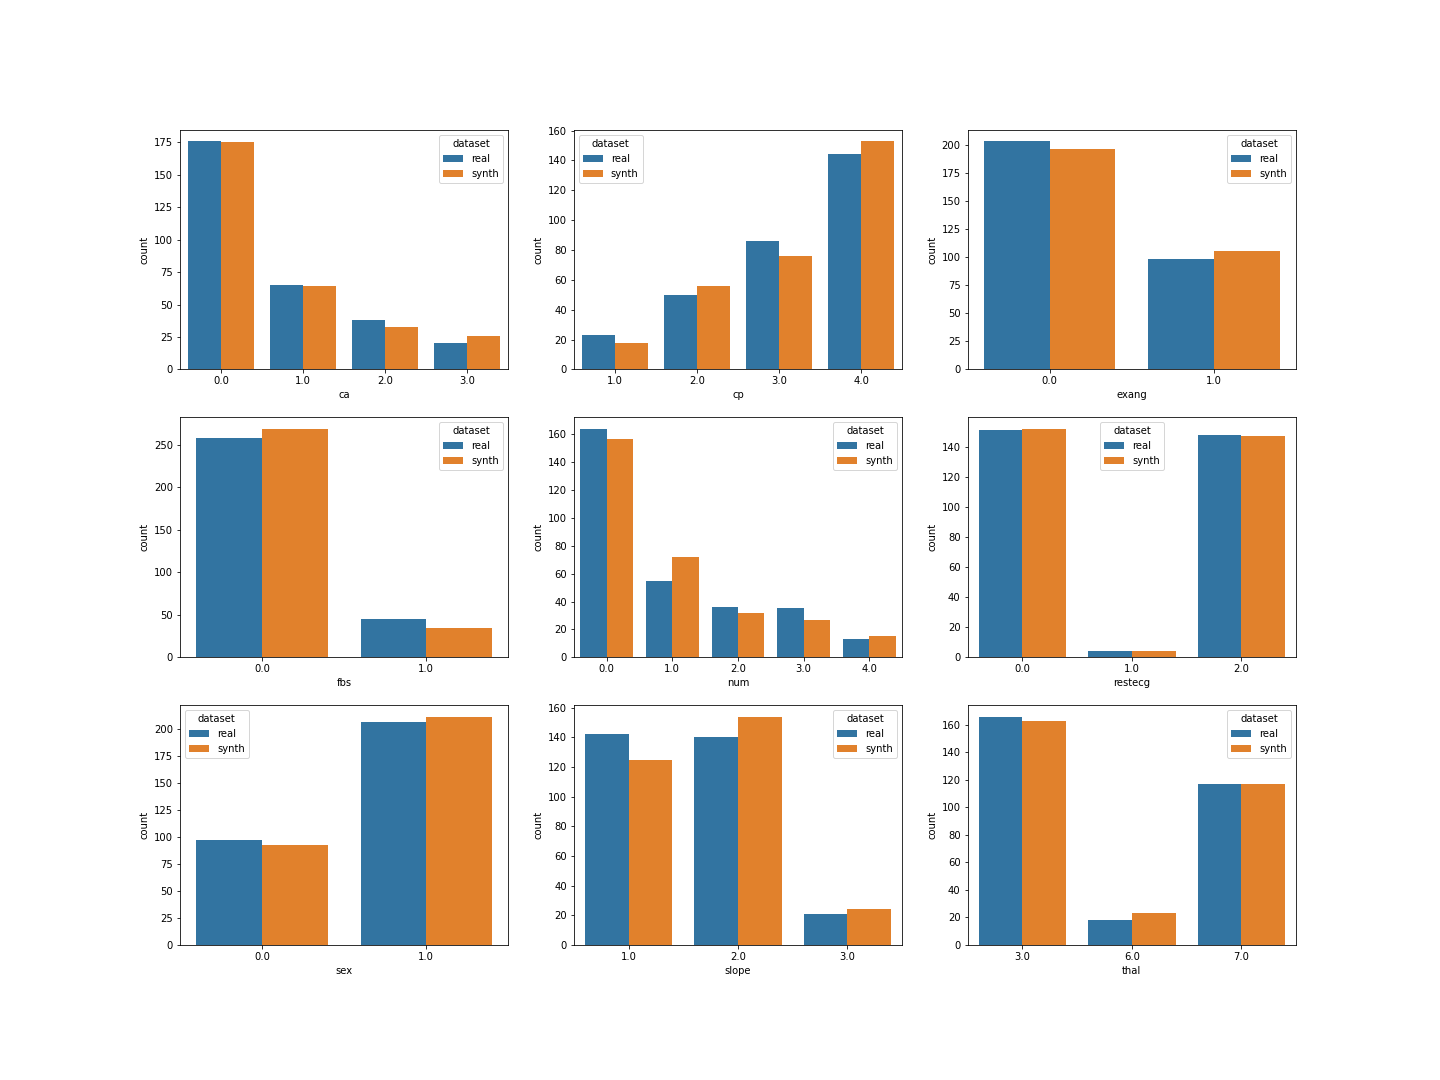
\includegraphics[scale=0.23]{figures/cat.png}
    \caption{Categorical Variables plotted}
    \label{fig:catgorical}
\end{figure}

\begin{figure}[t]
    \centering
    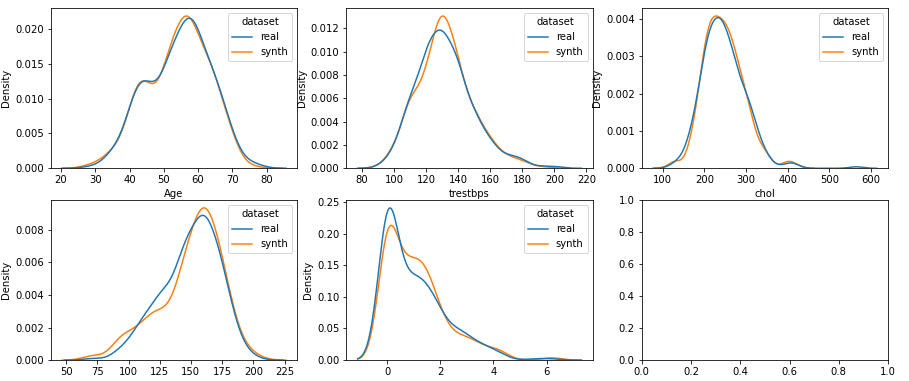
\includegraphics[width=\textwidth]{figures/continuous_plot_0.png}
    \caption{Continuous Variables plotted}
    \label{fig:continuous}
\end{figure}



\subsection{Discussion \& Conclusion}

The data possible to create to evaluate similarities between two datasets is important not only for synthetic vs real datasets. For example, in distributed learning, where different silos exist, with similar or even equal features, a method for evaluating the similarities can be useful for understanding how the populations are similar between them, trying to shed light on the most similarities among them, or different in order to understand the differences in the silos or data acquisition inside them.
Furthermore, the differences can be assessed on a more granular level. The column-wise similarities can be different from the inter-column similarities and this in itself, can be a metric of interest regarding the quality of the synthetic data and its generator.

With this work, we hope to help institutions and academics get access to a benchmark of the datasets provided in order to leverage synthetic data in the healthcare space. Finally, we hope this work helps other researchers reach an evaluation metric that could be a unique and clear response to the question of how similar two datasets are.




\section{Can We Use Machine Learning Feature to Compare Datasets?}\label{subsec:similarity}
This section is based on the paper entitled "Using Machine Learning Models' feature importance to assess dataset similarity". The reasoning behind this paper was the results of section \ref{subsec:gans}, where we felt that evaluation metrics for synthetic data could be improved. Better yet, we felt that the comparison of two datasets (that shared the same columns) could be done in a more robust way. Being that the current gold-standard was cross-validation which was not bound to any number range and the significance of the result could not be easily interpretable. We used the feature importance of several \ac{ml} models to compare datasets and concluded that it was a valid alternative to the traditional metrics.

\subsection{Introduction}
In recent years, the use of \ac{ai} and \ac{ml} algorithms has gained increasing prominence in healthcare research and practice. One of the key requirements for the successful application of these methods is access to large, high-quality datasets. However, in many cases, the availability of such datasets can be limited due to issues around data privacy, security, and ethical concerns \cite{chingOpportunitiesObstaclesDeep2018a}. To address this challenge, synthetic data has emerged as a promising solution. Synthetic data refers to artificially generated data that closely mimic the statistical properties and patterns of real-world data \cite{mullerEvaluationSyntheticElectronic2022}.

Synthetic data has the potential to overcome many of the limitations associated with real-world data, such as the lack of sufficient data volume, noise, and privacy concerns. Even though there are still doubts if the privacy part is the silver bullet sometimes referred to \cite{stadlerSyntheticDataPrivacy2020}, the upsampling part is a standard use for years now. However, the quality of synthetic data generated by various techniques can vary significantly, and it is essential to assess the quality of synthetic data before its usage. In healthcare, the assessment of synthetic data is crucial to ensure that it can provide valid insights and inform decision-making processes.

The assessment of synthetic data in healthcare is essential for its successful use in various applications, such as developing predictive models, testing algorithms, and conducting clinical trials. The use of synthetic data can significantly enhance the efficiency and effectiveness of healthcare research and practice. However, it is crucial to ensure that the synthetic data used in these applications are of high quality and validated to provide reliable and valid insights. The evaluation of synthetic data quality involves comparing its statistical properties and patterns with those of the original data. We can assess how similar columns are to each other through several statistical tests, and then we can infer some inter-column properties with methods like cross-validation, where two datasets are split into train tests and cross-tested and then the ratio between the evaluation result of both datasets is used as a metric.\cite{mullerEvaluationSyntheticElectronic2022,goncalvesGenerationEvaluationSynthetic2020a}. However, this methodology is a big proxy for such an inter-column relationship. Can we try to provide a better metric than this one to evaluate how similar are the inter-column relationship of two distinct datasets? In this paper, we suggest using feature importance values to create a more explainable and reasonable metric for inter-column relationships.

\subsection{Rationale and Related Work}
% !TeX root = ../../thesis.tex

Recently there has been a series of works related to assessing how synthetic data generators behave with data like the work of Emam et al. \cite{emamUtilityMetricsEvaluating2022} that especially focused on utility metrics for synthetic data generators. At the moment, comparing data is based on intra-columns and inter-columns relationship. The intracolumn relationship is assumed as something that compares equal columns between datasets, with highly known statistical methods like chi-squared or \ac{ks} like done in the works of \cite{combrinkComparingSyntheticTabular2022} among many others, acting more like sanity checks than anything else. 
Other known metrics are distance-based metrics like \ac{jsd}, Wasserstein Distance, Bhattacharyya Distance or Hellinger distance, which are based on the calculation of the distance between distributions like seen in the works of several teams \cite{ISI:000557358500024,choiGeneratingMultilabelDiscrete2017,Baowaly2019}.

However, regarding inter-column relationships, the metrics applied are often very different across papers. One example of trying to capture inter-column relationship is about the use of propensity score \cite{rosenbaumCentralRolePropensity1983,mullerEvaluationSyntheticElectronic2022} where a classifier is trained to the merged datasets, with the added variable of the original dataset (i.e., 1 for real and 0 for synthetic). The model is trained and the propensity Mean square error is the  mean squared difference of the estimated probability from the average prediction
Most recently, a unified metric appeared as the sum of other metrics known as described in the work of Chundawat et al., \cite{chundawatTabSynDexUniversalMetric2022}, known as TabSynDex. Other examples are likelihood of fitness like in the works of \cite{xuModelingTabularData2019b}, coverage support \cite{goncalvesGenerationEvaluationSynthetic2020a} or very specific metrics implemented for evaluating specific data generators.
However, the most used metric is cross-validation, which takes two datasets, one that is real and a second which is synthetic and we split both into train and test and train a machine learning model on the real data training set, then we test the model on both test sets. Then a ratio is created, rendering the actual value. This methodology, even if gold-standard at the moment for this type of study, has some liabilities since this value can be a bit erratic, and even above one since the evaluation metric could be better on the second dataset and we don't have a clear grasp of what that can represent in terms of dataset similarity. The image \ref{fig:1} represents this in detail. Several works used this metric as the comparing metric \cite{mullerEvaluationSyntheticElectronic2022}.

%TC:ignore
\begin{figure}[tbph]
\centering
\caption{Cross-Validation of datasets}\label{fig:1} 
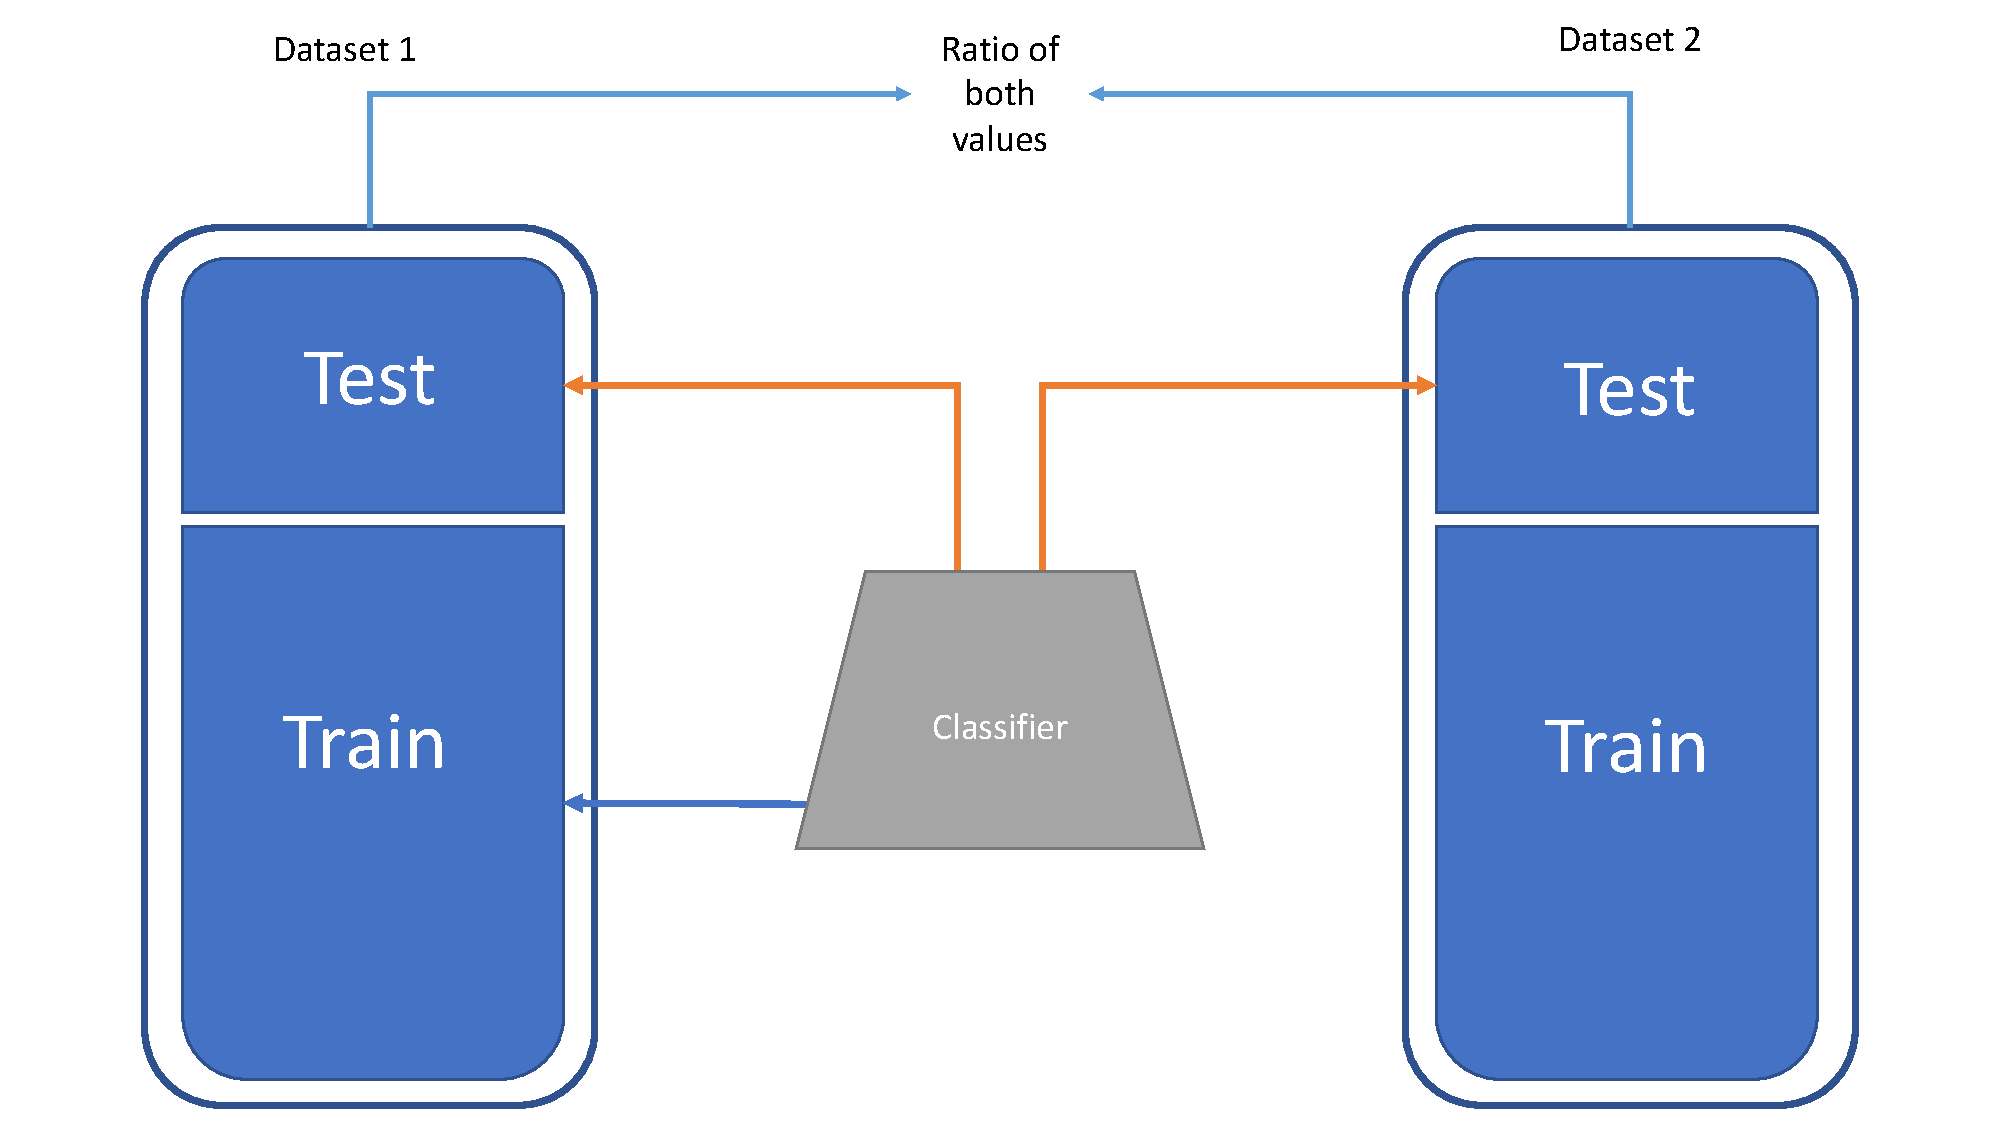
\includegraphics[scale=0.35]{figures/imagem1.pdf}
\end{figure}
%TC:endignore




%Utility Metrics for Evaluating Synthetic Health Data Generation Methods: Validation Study



\subsection{Materials \& Methods}
\subsubsection{Materials}
% !TeX root = ../../thesis.tex


We used 5 datasets from the UCI dataset repository. The ones chosen were related to healthcare and were heart disease \cite{misc_heart_disease_45}, thyroid disease \cite{misc_thyroid_disease_102}, liver disorders \cite{misc_liver_disorders_60}, breast cancer \cite{misc_breast_cancer_wisconsin_diagnostic_17} and the primary tumour dataset \cite{misc_primary_tumor_83}. These datasets were chosen due to three main reasons: 1) being open and facilitating recreation of results; 2) being tabular with mixed datatypes to better represent data in the real world and 3) diversity across domains inside healthcare (different diseases and contexts).

We made minimal preprocessing on the datasets, namely removing the missing variables by imputing the mean on continuous variables and mode on categorical.
We also created several synthetic datasets by applying known methods. Descriptive statistics of the datasets used are shown in table \ref{tab:descrptive_feature}.
\begin{small}    
\begin{table}[htpb]
    \footnotesize
        \caption{Descriptive statistics of datasets used. Mean (Standard Deviation) for continuous variables. Mode [nr categories] for categorical variables.}\label{tab:descrptive_feature}
            \begin{tabularx}{\textwidth}{lXll|lXll}
                \toprule
            Dataset & Column                         & Statistic    & \% Nulls & Dataset & Column          & Statistic    & \% Nulls \\
            \midrule
            heart   & Age                            & 54.4 (9.0)   & 0.0      & liver   & gammagt         & 38.3 (39.3)  & 0.0      \\
            heart   & sex                            & 1.0 {[}2{]}  & 0.0      & liver   & drinks          & 3.5 (3.3)    & 0.0      \\
            heart   & cp                             & 4.0 {[}4{]}  & 0.0      & liver   & Selector        & 2 {[}2{]}    & 0.0      \\
            heart   & trestbps                       & 131.7 (17.6) & 0.0      & thyroid & Class           & 1 {[}3{]}    & 0.0      \\
            heart   & chol                           & 246.7 (51.8) & 0.0      & thyroid & T3              & 109.6 (13.1) & 0.0      \\
            heart   & fbs                            & 0.0 {[}2{]}  & 0.0      & thyroid & TST             & 9.8 (4.7)    & 0.0      \\
            heart   & restecg                        & 0.0 {[}3{]}  & 0.0      & thyroid & TSTRI           & 2.1 (1.4)    & 0.0      \\
            heart   & thalach                        & 149.6 (22.9) & 0.0      & thyroid & TSH             & 2.9 (6.1)    & 0.0      \\
            heart   & exang                          & 0.0 {[}2{]}  & 0.0      & thyroid & TMAX            & 4.2 (8.1)    & 0.0      \\
            heart   & oldpeak                        & 1.0 (1.2)    & 0.0      & tumour   & class           & 1 {[}21{]}   & 0.0      \\
            heart   & slope                          & 1.0 {[}3{]}  & 0.0      & tumour   & age             & 2 {[}3{]}    & 0.0      \\
            heart   & ca                             & 0.0 {[}4{]}  & 1.3      & tumour   & sex             & 2 {[}2{]}    & 0.3      \\
            heart   & thal                           & 3.0 {[}3{]}  & 0.7      & tumour   & histologic-type & 2 {[}3{]}    & 19.8     \\
            heart   & num                            & 0 {[}5{]}    & 0.0      & tumour   & degree-of-diffe & 3 {[}3{]}    & 45.7     \\
            breast  & Clump Thickness               & 4.4 (2.8)    & 0.0      & tumour   & bone            & 2 {[}2{]}    & 0.0      \\
            breast  & Uniformity of Cell Size     & 3.1 (3.1)    & 0.0      & tumour   & bone-marrow     & 2 {[}2{]}    & 0.0      \\
            breast  & Uniformity of Cell Shape    & 3.2 (3.0)    & 0.0      & tumour   & lung            & 2 {[}2{]}    & 0.0      \\
            breast  & Marginal Adhesion             & 2.8 (2.9)    & 0.0      & tumour   & pleura          & 2 {[}2{]}    & 0.0      \\
            breast  & Single Epithelial Cell Size & 3.2 (2.2)    & 0.0      & tumour   & peritoneum      & 2 {[}2{]}    & 0.0      \\
            breast  & Bare Nuclei                   & 3.5 (3.6)    & 2.3      & tumour   & liver           & 2 {[}2{]}    & 0.0      \\
            breast  & Bland Chromatin               & 3.4 (2.4)    & 0.0      & tumour   & brain           & 2 {[}2{]}    & 0.0      \\
            breast  & Normal Nucleoli               & 2.9 (3.1)    & 0.0      & tumour   & skin            & 2 {[}2{]}    & 0.3      \\
            breast  & Mitoses                        & 1.6 (1.7)    & 0.0      & tumour   & neck            & 2 {[}2{]}    & 0.0      \\
            breast  & Class                          & 2 {[}2{]}    & 0.0      & tumour   & supraclavicular & 2 {[}2{]}    & 0.0      \\
            liver   & mcv                            & 90.2 (4.4)   & 0.0      & tumour   & axillar         & 2 {[}2{]}    & 0.3      \\
            liver   & alkphos                        & 69.9 (18.3)  & 0.0      & tumour   & mediastinum     & 2 {[}2{]}    & 0.0      \\
            liver   & sgpt                           & 30.4 (19.5)  & 0.0      & tumour   & abdominal       & 2 {[}2{]}    & 0.0      \\
            liver   & sgot                           & 24.6 (10.1)  & 0.0      &         &                 &              &          \\
              \bottomrule
            \end{tabularx}

        \end{table}
    \end{small}



\subsubsection{Method Overview}
For this work, our goal is to test several metrics based on the ranking of feature importance of a trained model. Normalized Discounted Cumulative Gain (NDCG) \cite{wangTheoreticalAnalysisNDCG} which is the sum of the true scores ranked in the order induced by the predicted scores, after applying a logarithmic discount. Then divide by the best possible score to obtain a score between 0 and 1. It is calculated by
\begin{equation}
\text{{NDGC}} = \frac{{\text{{DCG}}(P)}}{{\text{{IDCG}}(P)}}
\end{equation}
where $\text{{DCG}}(P)$ is the Discounted Cumulative Gain and $\text{{IDCG}}(P)$ is the Ideal Discounted Cumulative Gain. 

Cohen's kappa coefficient \cite{doi:10.1177/001316446002000104}  is a statistic that is commonly used to assess the level of agreement between two or more raters or evaluators who are providing categorical ratings or rankings of a set of items. So, we want to use to assess if it could be of use to check how similar the ranking of the features is, using the numbers as categorical.
\begin{equation}
\kappa = \frac{{P_o - P_e}}{{1 - P_e}}
\end{equation}

where \(P_o\) is the observed agreement between the two raters and \(P_e\) is the expected agreement between the two raters by chance.

We also intend to use the $R^2$ to check if the explainability changes across datasets.
\begin{equation}
R^2 = 1 - \frac{{\sum_{i=1}^n (y_i - \hat{y}_i)^2}}{{\sum_{i=1}^n (y_i - \bar{y})^2}}
\end{equation}


where \(y_i\) are the observed values of the dependent variable, \(\hat{y}_i\) are the predicted values of the dependent variable, \(\bar{y}\) is the mean of the observed values of the dependent variable and \(n\) is the number of data points.

Then we intend to use ranking metrics, namely Kendall tau, weighted Kendall tau and RBO.
Kendall tau is a measure of correlation that measures the similarity between two rankings. It is commonly used in statistics and data analysis to evaluate the agreement or disagreement between two sets of rankings.

The Kendall tau coefficient \cite{kendallTreatmentTiesRanking1945} is defined as the difference between the number of concordant and discordant pairs of observations, divided by the total number of pairs. A concordant pair is a pair of observations that have the same ranking order in both sets, while a discordant pair is a pair of observations that have opposite ranking orders. The Kendall tau coefficient ranges from -1 to 1, where -1 represents perfect negative correlation, 0 represents no correlation, and 1 represents perfect positive correlation. 
\begin{equation}
\tau = \frac{{\text{{number of concordant pairs}} - \text{{number of discordant pairs}}}}{{\text{{total number of pairs}}}}
\end{equation}

Weighted Kendall tau  \cite{vignaWeightedCorrelationIndex2015} is an extension of Kendall tau that takes into account the importance or weight of each observation in the rankings. In some cases, some observations may be more important than others, and their positions in the ranking may have a greater impact on the overall correlation. Weighted Kendall tau assigns a weight to each observation, and the correlation is calculated based on the weighted concordant and discordant pairs.
\begin{equation}
\tau_w = \frac{{\sum_{i<j} w_{ij} \cdot sgn(x_i - x_j)}}{{\sum_{i<j} w_{ij}}}
\end{equation}

where $w_{ij}$ is the weight associated with the pair $(x_i, x_j)$ and $sgn(\cdot)$ is the sign function.
Rank-biased overlap (RBO) \cite{webberSimilarityMeasureIndefinite2010} is a measure of similarity between two ranked lists or rankings. It takes into account the order of items in the two lists, and it can be used to evaluate the quality of search results, recommendations, or any other kind of ranked list it has been shown to be more robust and accurate than other similarities measures such as Kendall tau or Spearman's rank correlation coefficient. 
\begin{equation}
\text{{RBO}} = (1 - \rho) \cdot \sum_{d=1}^{\infty} \left( \frac{{g_d}}{{d}} \right) \cdot \rho^d
\end{equation}

where $\rho$ is the weight, $g_d$ is the gain at depth $d$, and $\sum_{d=1}^{\infty}$ indicates the summation over all depths.


Finally, we intend to use text-distance metrics. The theory behind this experiment is to treat the ordered columns in a ranking manner and apply text-distance metrics to check the distance between the two. Levenshtein distance \cite{navarroGuidedTourApproximate2001} is the minimum number of single-character insertions, deletions, or substitutions required to transform one string into another. Damerau-Levenshtein distance \cite{navarroGuidedTourApproximate2001} is similar to Levenshtein distance but also includes the transposition of two adjacent characters as an allowable operation. The hamming distance \cite{6772729} is a measure of the difference between two strings of equal length, defined as the number of positions at which the corresponding symbols are different. Jaro-Winkler distance \cite{navarroGuidedTourApproximate2001} is a string similarity measure that takes into account the number of matching characters, the number of transpositions, and the length of common prefixes, with a higher weight given to the common prefix.




\begin{algorithm}[hbtp]
\SetAlgoLined

\For {i in number of columns to test}{
\For {rep in  10 repetitions}{ 
permutate values in i columns

\For {dataset in dataset pair}{

\For {target in dataset columns}{

Train-Test Split (95:5)
 model fit to train
     get feature importance per column
     Create an ordered rank of features 
 }}}}


 \caption{Testing similarity scores in tabular datasets}
 \label{alg:simil_1}

\end{algorithm}



The algorithms chosen were decision trees, random forests, \ac{svm},  \ac{knn}, and linear regression/logistic regression as implemented in the \textit{scikit-learn} package \cite{scikit-learn}. The text distance metrics were implemented by the text-distance package \cite{orsiniumTextdistanceComputeDistance}. Kendall tau, weighted Kendall tau were used as implemented by scipy \cite{virtanenSciPyFundamentalAlgorithms2020a} and RBO, as implemented in \cite{chenRankbiasedOverlapRBO2023}.








\subsection{Results}
With the method described in the algorithm \ref{alg:simil_1}, we created a figure where the metrics are presented with increasingly different datasets: figure \ref{fig:lineplot}.
%Then we compared the difference in the metric across iterations, rendering figure \ref{fig:boxplot}.


%TC:ignore
\begin{figure}[htbp]
\centering
\caption[Plot showing the decrease of the metric over increasingly changed datasets.]{Plot showing the decrease of the metric over increasingly changed datasets. The X axis represents the number of columns mutated. The Y axis represents the value of the metric and the hue represents the algorithm used to calculate the metric.}\label{fig:lineplot} 
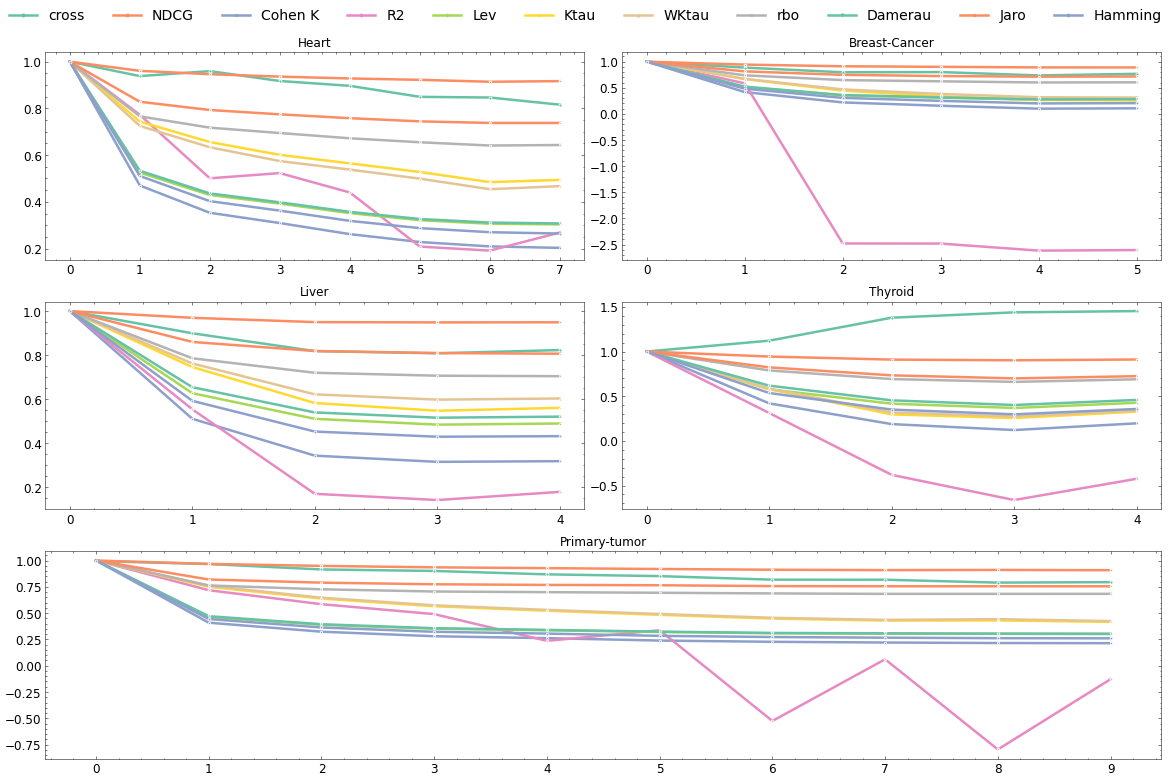
\includegraphics[scale=0.37]{figures/multiple_datasets.png}
\end{figure}
%TC:endignore


%TC:ignore
\begin{figure}[htbp]
\centering
\caption{Plot showing the values at 50\% columns mutated across all datasets and algorithms per metric type}\label{fig:boxplot} 
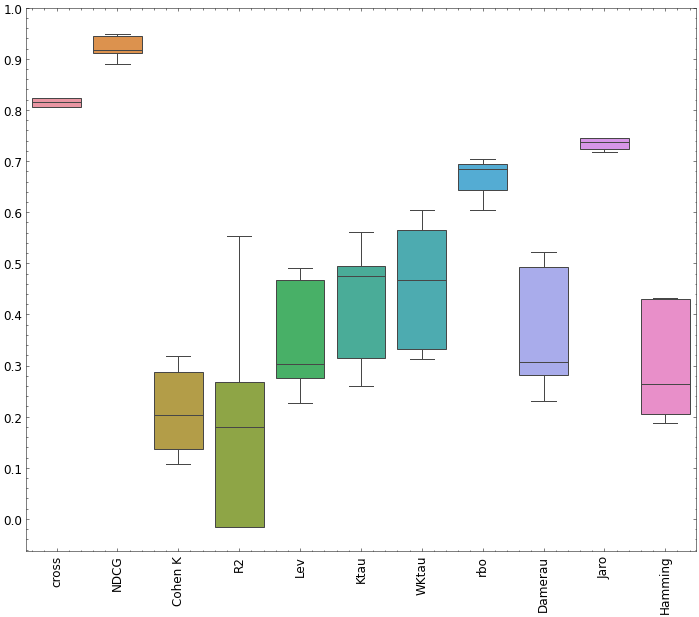
\includegraphics[scale=0.55]{figures/50_percent_data.png}
\end{figure}
%TC:endignore


The number of repetitions and how that impacts the variance of the scores is shown in figure \ref{fig:facet_plot}.






%TC:ignore
\begin{figure}[htbp]
\centering
\caption{Plot the variance of different repetitions for every metric and the number of different columns changed. X is the number of columns mutated. Colour is the number of repetitions for each mutation and Y is the variance of the data. }\label{fig:facet_plot} 
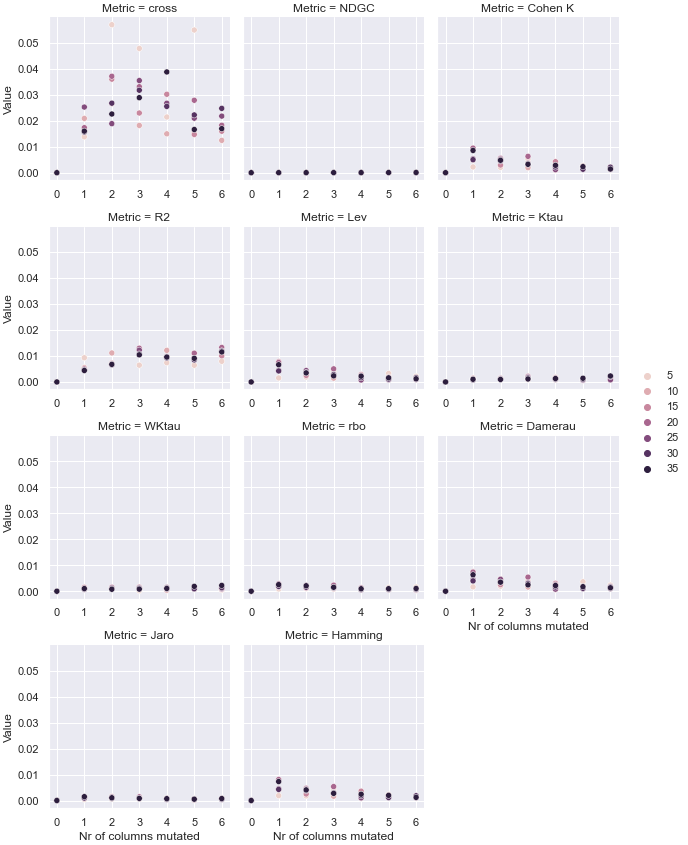
\includegraphics[scale=0.55]{figures/facet_plot.png}
\end{figure}
%TC:endignore

As for the test for the synthetic and real datasets, the results are displayed in figure \ref{fig:synth_result}.
%TC:ignore
\begin{figure}[htbp]
\centering
\caption{Result on a synthetic and real data }\label{fig:synth_result} 
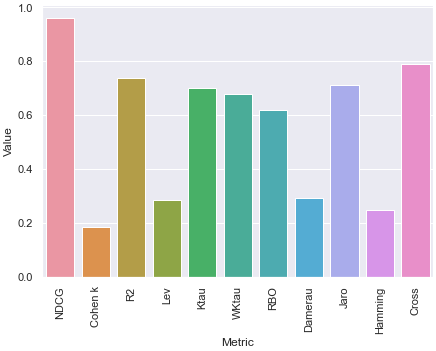
\includegraphics[scale=0.65]{figures/synthetic.png}
\end{figure}
%TC:endignore
\subsection{Discussion}
% !TeX root = ../../thesis.tex


With the results found, we feel that are better alternatives to CC. \ac{rbo} seems like alternatives to CC. Firstly, as with Kendall tau and Weighted Kendall tau, it seems to be directly connected to a difference in the dataset. They seem to lower from 1 (equal datasets) to around 50\% when the columns changed are half of the columns of the dataset, which seems an encouraging result. Secondly, it is a bounded metric between 0 and 1, which is helpful for interpretation since, as we have seen with for example CC and $R^2$, they can go outside these bounds, making  the interpretation of the results more difficult for these scenarios. Thirdly, variance across different iterations is also lower. Even though the variance across all metrics is quite low (except $R^2$), \ac{rbo} seems to have less variance than Kendall tau and Weighted Kendall tau, which could be the differentiating factor between these 3 metrics.  With CC, we have a variance that despite low (on the 0.01 level), is still higher than the other metrics (except $R^2$) which have variance around 0. This is important, since it is independent of numbers of runs to get a stable result.
Regarding text metrics, they have a drastic drop with only one column mutated (Figure~\ref{fig:lineplot}) but the decrease is steady afterwards. As for $R^2$, we see that it is not a good metric for this type of problem, since it is not bounded between 0 and 1, and it has a high variance across different iterations. This is probably due to the fact that it is a regression metric, and it is not designed for this type of problem.

While the proposed metrics such as \ac{rbo} and Kendall Tau have shown promise in capturing changes in feature importance, there are several limitations that should be addressed in future research. 
Firstly, the possibility of synthetic datasets may be different in other ways that a value permutation could not grasp. For example, the distribution of the data could be different, or the number of unique values could be different. Nevertheless, we tested with 3 sets of synthetic datasets produced by us as counterpart to the 5 original datasets to make at least a sanity check that the new approaches assessed are at least in tune with CC for actual synthetic datasets (Figure~\ref{fig:synth_result} and \ref{fig:synth_heat}). We can see that the values are at least near the values of CC. Moreover, they seem to have less variability, which can make sense taken into account the synthetic data generator was the same. These results also point towards the direction that these new approaches could be a good alternative to CC.

Secondly, the metrics have primarily been tested on synthetic datasets, and their performance on real-world datasets with varying distributions, noise, and missing data remains to be fully explored. Thirdly, these metrics may not fully account for complex interactions between features, which are often present in real-world datasets. Future work could focus on incorporating feature interaction measures or combining these metrics with statistical distance metrics to better reflect such complexities. Additionally, while the variance of the proposed metrics is generally low, exploring methods to further reduce variance, especially in high-dimensional datasets, would enhance their robustness. Finally, future research could develop methods to provide confidence intervals or uncertainty estimates for these metrics, which would improve their interpretability and reliability in practical applications.


With these findings, we believe that progress has been made in comparing tabular datasets, which may prove beneficial not only for evaluating synthetic data generators but also for formalizing the degree of similarity between datasets that share common features. This approach provides a valuable reference for the development of new data generators and enhances confidence in benchmarks and comparisons.
\subsection{Conclusion}
% !TeX root = ../../thesis.tex

Comparing two tabular datasets has been growing in demand in the past year mainly because of the increase in popularity of tabular data synthesis methods which have exhibited the potential in generating valuable synthetic data. However, due to the absence of a uniform metric, evaluating different methods has been inconsistent. This research proposes some alternatives for assessing synthetic tabular data's utility. \ac{rbo} seems to have the potential to capture inter-column relationships in a more consistent way than cross-classification. They could become a useful tool for comparing statistical methods of generating synthetic tabular data. Furthermore, this metric can aid in evaluating these generators' training, providing insights into improving synthetic data quality. The proposed metrics open up possibilities for future research to enhance tabular data synthesis methods and compare two datasets overall. Future research could be expanded in new comparison with others evaluation metrics, other datasets and other synthetic data generators.


\section{Can We Use Machine Learning To Create Automatic Data Quality Assessments?}\label{subsec:dq}
This section is based on the paper entitled "Development and Validation of a Data Quality Evaluation Tool in Obstetrics Real-World Data through HL7-FHIR interoperable Bayesian Networks and Expert Rules" This paper focuses on the fact that data quality is a major concern in healthcare. We developed a tool that could be used to assess the quality of data in a \ac{ehr} and provide a report on the quality of the data. We used a combination of \ac{bn} and expert rules to assess the quality of the data. Furthermore, we tested the tool on 9 real-world datasets of obstetrics \acp{ehr} and concluded that the tool was a valid alternative to the traditional methods of assessing data quality.
%\input{chapters/data-quality-paper}
\subsection{Introduction}
With the wide spreading of healthcare information systems across all contexts of healthcare practice, the production of health-related data has followed this incremental behaviour. The potential for using this data to create new clinical knowledge and push medicine further is tempting \cite{martin-sanchezBigDataMedicine2014}.
However, to correctly use the data stored in \acp{ehr}, the quality of the data must be robust enough to sustain the clinical decisions made based on this data. Data quality cannot be construed as a linear concept; it is intrinsically dependent on the context in which it is evaluated. The quality thresholds and dimensions required to classify the quality of the data depend on the purpose that we intend to use that very same data \cite{waljiElectronicHealthRecords2019}. These uses can be very distinct and have different impacts as well. For one, we can use data to support day-to-day decisions regarding individual patients’ care \cite{verheijPossibleSourcesBias2018}. These decisions can include ones based on recorded information to understand a patient’s history, clinical decision support systems based on this data, or even using the data to help support a more macro, public health-oriented decision. Another area is using information for management purposes. The data can be used by management bodies and regulatory authorities to extract metrics regarding the quality of care or reimbursement purposes. Thirdly, data can be used for research purposes, namely observational studies and, more recently, to support clinical trials through real-world evidence analysis \cite{coreyAssessingQualitySurgical2020,verheijPossibleSourcesBias2018,wengClinicalDataQuality2020}. 
So, all the \ac{ehr} data-based decisions can only be as good as the data supporting them. Several studies have already warned about the lack of data quality in \acp{ehr} and how this can be a significant hurdle to an accurate representation of the population and potentially lead to erroneous healthcare decisions \cite{reimerDataQualityAssessment2016a,joukesImpactElectronicPaperBased2019a,huserMultisiteEvaluationData2016,zhangUnderstandingDetectingDefects2020,kramerImpactDataQuality2021,gigantiImpactDataQuality2019}.

There are several steps in the data lifecycle that can be prone to error, from data generation, where the data is registered by healthcare professionals, passing by data processing, whether inside healthcare institutions or by software engineers aiming to reuse data, to data interpretation and reuse, where investigators
try to interpret the meaning of registered data\cite{wengClinicalDataQuality2020}.
So, with all of the data’s possible uses added to the several steps that can introduce errors throughout the data lifecycle, data quality frameworks and sequential implementations can have very distinct approaches and methodologies to assess data quality. Data quality tools for checking data being registered live to support day-to-day decisions will be significantly different from one whose only purpose is to provide quality checks for research purposes. So, methodologies to tackle these issues are necessary for guaranteeing the quality of healthcare practice and the knowledge derived from \ac{ehr} data. Consequently, in this paper, we propose:
\begin{myitemize}
    \item Create a tool for identifying data quality issues in obstetrics \acp{ehr};
    \item Enlighten on the issues that can appear with a full deployment of such a tool
    \item Suggestion of a creation of a single score for data quality for comparison of high-quality and low-quality records in a database.
    \item Assess how such a tool can work in early-stage real-world scenarios and how to work with obstetricians to improve data quality.
    \item Identify data quality issues on obstetrics data
\end{myitemize}


%Data quality is a crucial aspect of the healthcare industry, as it impacts the accuracy of diagnoses, treatment plans, and patient outcomes. The reliability and accuracy of healthcare data have far-reaching consequences, including financial implications, patient safety, and legal ramifications. Inaccurate or incomplete data can lead to incorrect diagnoses, inappropriate treatments, and ultimately harm to patients. Therefore, ensuring the quality of healthcare data is essential to providing effective and safe healthcare services.

%One of the main reasons why data quality is so critical in healthcare is that healthcare data is often used to make important decisions, such as treatment plans, patient management, and resource allocation. Inaccurate or incomplete data can lead to misdiagnosis, inappropriate treatment, and increased healthcare costs. Furthermore, inaccurate data can hinder research efforts and impede the development of new treatments and therapies.

%Another key aspect of data quality in healthcare is its role in patient safety. Accurate and reliable data is essential for ensuring patient safety, particularly in areas such as medication management, clinical decision-making, and adverse event reporting. Poor data quality can lead to medication errors, adverse drug reactions, and other types of harm to patients.

%Finally, data quality is also important for legal and regulatory compliance in healthcare. Accurate and complete data is required for compliance with regulations such as HIPAA, the Affordable Care Act, and other regulatory requirements. Poor data quality can result in legal and financial penalties, as well as reputational damage for healthcare organizations.

%Overall, data quality is a crucial aspect of healthcare, with far-reaching implications for patient safety, healthcare costs, and regulatory compliance. Ensuring the quality of healthcare data requires a comprehensive approach that includes data governance, data management, data quality assurance, and ongoing monitoring and improvement efforts. By prioritizing data quality, healthcare organizations can provide better patient care, improve outcomes, and reduce costs.





\subsection{Background and Related Work}
There is already a significant number of papers trying to define data quality assessment frameworks for \ac{ehr} data, all of them plausible and recommendable, already described in other papers \cite{bianAssessingPracticeData2020}. The literature has over 20 different methods, descriptions, and summaries of  different frameworks over the years. Some may be highlighted from the review from Weiskopf et. al, \cite{weiskopfMethodsDimensionsElectronic2013}, where five data quality concepts were identified over 230 papers: Completeness, Correctness, Concordance, Plausibility and Currency. 



The work of Saez et al. defined a unified set of \ac{dq} dimensions: completeness, consistency, duplicity, correctness, timeliness, spatial stability, contextualization, predictive value, and reliability \cite{saezOrganizingDataQuality2012}. Then a review of Bian et al. \cite{bianAssessingPracticeData2020} expanded on the previous ones, categorizing data quality into 14 dimensions and mapping them to the previous most known definitions. These were: currency, correctness, plausibility, completeness, concordance, comparability, conformance, flexibility, relevance, usability, security, information loss, consistency, and interpretability.

Finally, the work of Khan et al. tried to harmonize data quality assessment frameworks, which simplified all previous concepts into three main categories: Conformance, Completeness and Plausibility and two assessment contexts: Verification and Validation \cite{kahnHarmonizedDataQuality2016a}.
Despite all of these comprehensive works, there is still no consensus regarding which one is best or which has taken the lead in usage. Moreover, looking at all of the descriptions related in the literature, a significant portion of concepts are overlapping, and sometimes hard to conceptualize such dimensions in practice.

As for implementations, there are already some available, such as the work from \cite{phanAutomatedDataCleaning2020} where a tool created by primary care in the Flanders was built to assess completeness and percentage of values within the normal range.
The work from Liaw et al. \cite{liawQualityAssessmentRealworld2021} already reviewed some data quality assessment tools, like tools from OHDSI \cite{hripcsakObservationalHealthData2015} or TAQIH \cite{alvarezsanchezTAQIHToolTabular2019}. 
Additionally, we found some others with similar purposes and characteristics like the work presented data dataquieR \cite{schmidtFacilitatingHarmonizedData2021}, an R language-based package that can assess several data quality dimensions in observational health research data. 
Also, the work from Razzaghi et al. developed a methodology for assessing data quality in clinical data \cite{razzaghiDevelopingSystematicApproach2022}, taking into account the semantics of data and their meanings within their context. Furthermore, the work from Rajan et al. \cite{rajanContentAgnosticComputable2019} presented a tool that can assess data quality and characterize health data repositories. Parallel to this, Kaspner et al. created a tool called DQAStats that enables the profiling and quality assessment of the MIRACUM database, being possible to integrate into other databases as well \cite{kapsnerLinkingConsortiumWideData2021a}.

Regarding data quality assessment as a whole, the works of \cite{estiriSemisupervisedEncodingOutlier2019}, focused on outlier detection in large-scale data repositories. The works of \cite{saezEHRtemporalVariabilityDelineatingTemporal2020} focused on the exploration and identification of dataset shifts, contributing to the broad examination and repurposing of large, longitudinal data sets. The works of García-de-Léon-Chocano \cite{saStandardizedDataQuality2017,garcia-de-leon-chocanoConstructionQualityassuredInfant2016,garci;a-de-leon-chocanoConstructionQualityassuredInfant2015} are the only ones focused on obstetrics data, but aimed to improve the process of generating high quality data repositories for research and best practices monitoring. These are similar and complementary works to this one. Finally, the work of \cite{springateREHRPackageManipulating2017} focused on the manipulation of \ac{ehr} data, including data quality assessment, data cleaning, and data extraction. However, these tools are not meant to be used at the production level, assessing data as it is being registered or outputs reports for human consumption and not a quantitive metric for metric comparison. Furthermore, none of these tools had standard-based interoperability in mind. Finally, we have not seen, until the moment of this paper, any implementation that used machine learning to evaluate the correctness of the value.

\subsection{Materials}
The data was gathered from 9 different Portuguese hospitals regarding obstetric information: data from the mother, several data points about the fetus and delivery mode. The data is from 2019 to 2020. The software for collecting data was the same in every institution, and the columns were the same, even though the version of each software differed across hospitals. Across the different hospitals, data rows ranged from 2364 to 18177. The sum of all rows is 73351 rows.  The data dictionary is in appendix \ref{appendix:data_dict}. This study received Institutional Review Board approval from all hospitals included in this study with the following references: Centro Hospitalar São João; 08/2021, Centro Hospitalar Baixo Vouga; 12-03-2021, Unidade Local de Saúde de Matosinhos; 39/CES/JAS, Hospital da Senhora da Oliveira; 85/2020, Centro Hospitalar Tâmega Sousa; 43/2020, Centro Hospitalar Vila Nova de Gaia/Espinho; 192/2020, Centro Hospitalar entre Douro e Vouga; CA-371/2020-0t\_MP/CC, Unidade Local de saúde do Alto Minho; 11/2021. All methods were carried out in accordance with relevant guidelines and regulations.
Data was anonymized before usage. 
For this purpose, we took the Khan harmonized framework since we understood it as simpler to communicate, we feel that the three main categories are indeed non-reducible, which makes sense from an organizational standpoint. Furthermore, the work done by Khan et al. with mapping to already existing frameworks could help compare this work with others who felt the need to use other frameworks. With this in mind, we will use three main categories, Completeness, Plausibility and Conformance. Completeness relates to missing data. Plausibility relates to how believable the values are. Conformance relates to the compliance of the data representation, like formatting, computational conformance and other data standards implemented. 

%TC:ignore
\begin{figure}[htbp]
\centering
\caption{Dimensions of data quality}\label{fig:categories} 
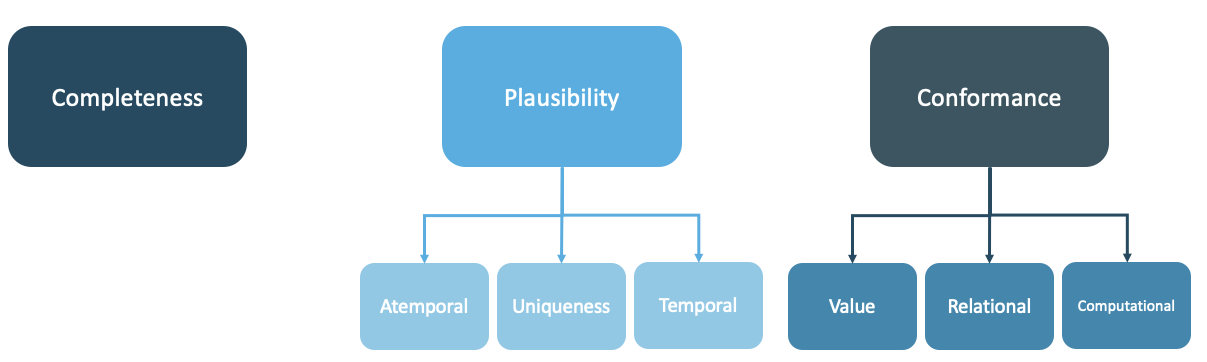
\includegraphics[scale=0.29]{figures/data-quality-v1.png}
\end{figure}
%TC:endignore
\subsection{Methods}
% !TeX root = ../../thesis.tex

For completeness, we used the inverse of the percentage of nulls in the training set. For plausibility, several methods were applied. The first was a Bayesian network. 

In our approach, Bayesian networks, which are probabilistic graphical models, play a pivotal role in predicting the plausibility of different elements. These networks are structured as directed acyclic graphs, where each node represents a variable and edges denote conditional dependencies among these variables \unskip~\cite{pearl1988probabilistic}. This structure allows the network to efficiently manage and represent the probabilistic relationships between multiple variables. The core strength of Bayesian networks in our context lies in their ability to predict the plausibility of various elements by analyzing these interdependencies. By integrating the conditional probabilities of variables and their dependencies, the network can infer the likelihood of certain outcomes or states, thereby assessing the plausibility of different columns in our dataset, when compared with the registered value. 

With this, we hope to capture the heterogeneous essence of the data, as well as possible outliers that are also plausible. We chose this model for its dual advantages: its capability to classify the plausibility of all columns within a single unified framework, and its interpretability, which allows for a clearer understanding of how each variable influences the overall plausibility prediction. The networks were created with the pgmpy package \unskip~\cite{pgmpy}. 

Secondly, we added the outlier-tree method\unskip~\cite{cortesExplainableOutlierDetection2020} which tries to integrate a decision tree that ''predicts'' the values of each column based on the values of each other column. In the process, every time separation is evaluated, it takes observations from each branch as a homogeneous cluster to search for outliers in the predicted 1-d distribution of the column. Outliers are determined according to confidence intervals in this 1-d distribution and need to have large gaps in order to be marked as outliers in the next observation. Because it looks for outliers in the branch of the decision tree, it knows the conditions that make it a rare observation relative to other observation types corresponding to the same conditions, and these conditions are always related to target variables (as predicted by them).  As such, it can only detect outliers described by decision tree logic, and unlike other methods such as isolation forests, it can not assign outlier points to each observation, or detect outliers that are generally rare, but will always provide human-readable justification when it recognizes outliers. Therefore, these methods not only identify anomalies based on a single column/variable but also consider the context of the data, providing a more nuanced understanding of what constitutes an outlier. This contextual awareness ensures that the outliers are not merely statistical deviations but are also substantively significant within the specific framework of the target variables. 

We added also elliptic envelope and Local Outlier Factor as complementary models to these two. Elliptic envelope is a method that assumes a Gaussian distribution of data, fitting an ellipse to the central data points to identify outliers. It works best with normally distributed data but is less effective in higher dimensions or non-normal distributions. Local Outlier Factor measures the local density deviation of a data point relative to its neighbors, identifying outliers without assuming a specific data distribution. It is versatile for different data structures but sensitive to parameter settings, like the number of neighbors. 

An Interquartile Range (IQR) based metric was also added as a supportive metric. This metric used the difference between Q1 and the triple of IQR  to define a lower threshold and Q3 + 3IQR to define an upper threshold. We only categorized as outlier the values that fell outside these margins. Finally, a rule system was implemented to leverage domain knowledge in the overall scoring. The system is based on great expectations package \unskip~\cite{GXProactiveCollaborative}. A set of 17 rules was defined by the team, focusing on impossible numbers or relationship between variables  or value format. The rules covered plausability and conformance. 

The Conformance-based were related to technical issues like the format of dates (date of birth like d/m/y), and conformance to the value set (i.e. Robson group, bishop scores, or delivery types). Plausibility rules were linked to expected values for BMI, weight, and gestational age (gestational age between 20 and 44). We also added plausibility for the relationship between columns, namely weight across different weeks of gestation (weight week 35 {\textgreater} weight week 25). We have also added a relationship of greatness between ultrasound weights more than 5 weeks apart. 

As for preprocessing, all null representations were standardized, we also removed features with high missing rates ({\textgreater} 80\% ). The imputation process was performed with the median for continuous and a new category (NULLIMP) for categorical variables.

For the usage of the Bayesian network in particular, the continuous variables were discretized into three bins defined by quantile. We defined three as the number of bins in order to reduce the number of states in each node of the network. The evaluation was done with cross-validation with 10 splits and two repetitions for each column as the target.

The API for serving the prediction models was developed with FastAPI. So, the methods applied in terms of the DQA framework shown in figure \ref{fig:categories} are described in the table \ref{tab:methods}.

\begin{table}[htpb]
\caption{Implemented Methods in the tool. The first column is the category or data quality dimension. The second is a subcategory of the first column if applicable and the third column is the actual method used to assess such a dimension.} \label{tab:methods}
\renewcommand{\arraystretch}{1.4}
\setlength{\tabcolsep}{10pt}

\begin{tabularx}{\textwidth}{ p{2cm} p{3.5cm} X }
\hline
 Category   & Subcategory           & Method   \\ \hline
Completeness     & N/A               & Score by the inverse percentage of missing in the train data         \\ 
Plausibility & Atemporal Plausibility & Bayesian model prediction based on the other values of row \\ 
Plausibility & Atemporal Plausibility         & Z-score for column value based on IQR train data       \\    
Plausibility & Atemporal Plausibility           & Elliptic Envelope                       \\ 
Plausibility & Atemporal Plausibility           & Local Outlier Factor                \\ 
Conformance & Value Conformance           & Manual Rule engine                           \\ 
Plausibility & Atemporal Plausibility           & Manual Rule engine                      \\ 
Plausibility & Atemporal Plausibility           & outlier-tree                      \\ 
Conformance & Value Conformance & Manual Rule engine\\
\hline
\end{tabularx}

\end{table}


For trying to compile all of these models into a single value, that could grasp the quality of the row or patient, a scoring method was created. The method of calculating the final score is stated in figure \ref{fig:scoring_method}. 
%TC:ignore
\begin{figure}[htbp]
    \centering
    \caption{Workflow and weights used for creating the final score and which elements are used to do so.}\label{fig:scoring_method} 
    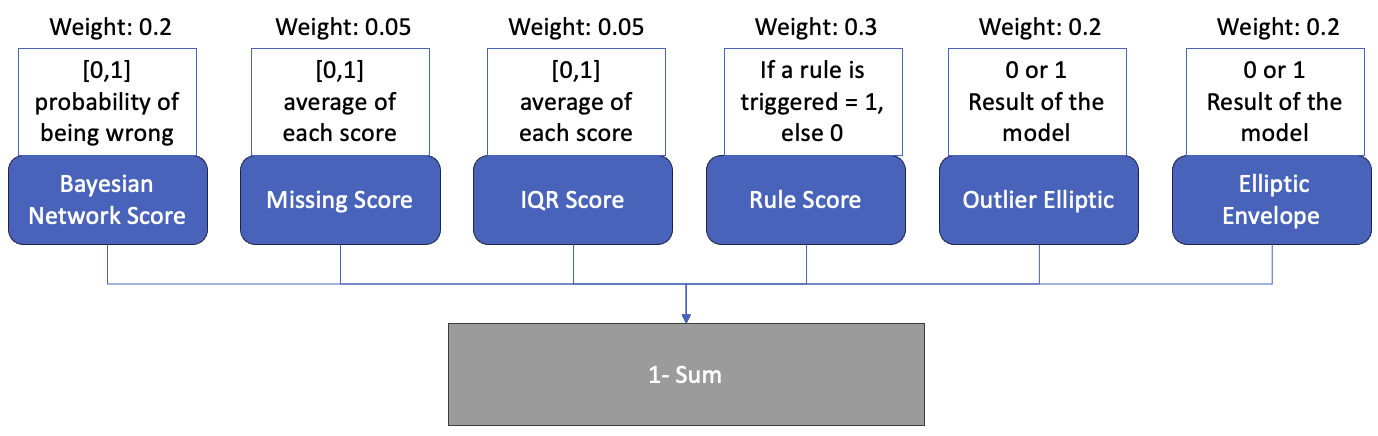
\includegraphics[scale=0.29]{figures/score-method.png}
    \end{figure}
    %TC:endignoregrama

To assess the tool's usefulness, we implemented it in a production environment and collect metrics regarding the data being produced. Then we presented some rows (or patient's records) to selected obstetrics clinicians for them to assess how likely the information is to be suitable for usage and rank it according to the perceived quality of the record. This was done through questionnaire, presenting the data and asking the clinicians to rank them from 1-10 and to describe the most important feature for the decision. We then compared the results with the ones from the model to make sanity checks regarding the model's performance and adequacy. We used Kendal Tau and Average Spearman's Rank Correlation Coefficient. Kendall Tau is a non-parametric statistic used to measure the strength and direction of the association between two ordinal variables. It calculates the difference between the number of concordant and discordant pairs of observations, normalized to ensure a value between -1 (perfect disagreement) and 1 (perfect agreement). Spearman's rank correlation coefficient is a non-parametric measure that assesses the strength and direction of a monotonic relationship between two ranked variables. It is based on the ranked values of the variables rather than their raw data, producing a value between -1 (perfect inverse relationship) and 1 (perfect direct relationship). Finally, we tested the capability of the model to discriminate bad quality records from good quality records, testing various thresholds of rank of quality, taken into account physicians responses.
We wrote all the code in Python 3.10.6 with the usage of the scikit-learn library for preprocessing, and evaluation\unskip~\cite{scikit-learn}.

\subsection{Results}

A \ac{bn} with structure and parameters learned from the training dataset reached an average \ac{auroc} of 0.857. The results are in the table \ref{tab:result_auc}.



\begin{table}[htpb]
 \caption{Validation Results: Column acronym with \ac{auroc} along with 95\% \ac{ci}. Acronym description is available in appendix \ref{appendix:data_dict}} \label{tab:result_auc} 

\renewcommand{\arraystretch}{1.2}
%\setlength{\tabcolsep}{8pt}
\centering
\begin{tabular} { p{1.5cm} p{1.5cm} p{3cm} p{1.5cm} p{1.5cm} l }
\hline
AP & 0.944 & [0.943, 0.945] & VNH & 0.894 & [0.893, 0.895] \\
AG & 0.797 & [0.778, 0.816] & TPEE & 0.816 & [0.815, 0.816] \\
EA & 0.969 & [0.968, 0.969] & AA & 0.751 & [0.743, 0.758] \\
CA & 0.958 & [0.958, 0.958] & GR & 0.931 & [0.93, 0.932] \\
IA & 0.638 & [0.637, 0.638] & V & 0.983 & [0.982, 0.983] \\
PI & 0.881 & [0.88, 0.881] & TP & 0.866 & [0.865, 0.868] \\
IMC & 0.881 & [0.881, 0.882] & VCS & 0.79 & [0.789, 0.791] \\
NRC & 0.75 & [0.75, 0.75] & ANP & 0.942 & [0.938, 0.946] \\
IGA & 0.968 & [0.968, 0.969] & GS & 0.514 & [0.507, 0.52] \\
SGP & 0.974 & [0.974, 0.974] & S & 0.896 & [0.896, 0.897] \\
VA & 0.974 & [0.974, 0.974] & VP & 0.771 & [0.77, 0.772] \\
TG & 0.728 & [0.726, 0.73] & TPNP & 0.952 & [0.951, 0.952] \\
\hline
 \multicolumn{6}{c}{\textbf{Average}  \textbf{0.857 [0.846, 0.868]}} \\

\hline
\end{tabular}
\end{table}


The network is as represented in figure \ref{fig:network}.
%TC:ignore
\begin{figure}[htbp]
\centering
\caption{Network learned}\label{fig:network} 
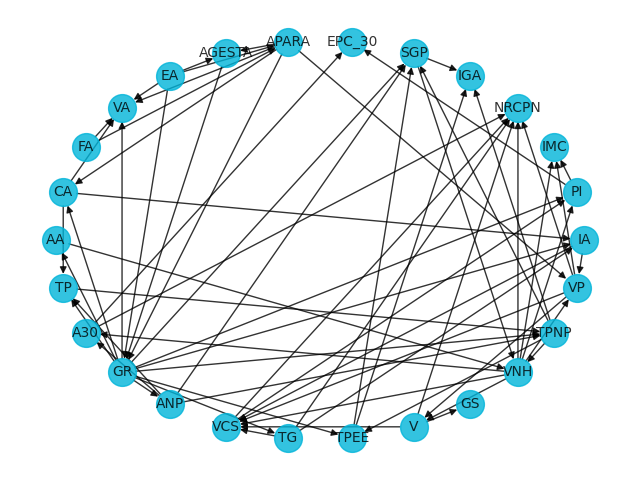
\includegraphics[scale=0.68]{figures/network.png}
\end{figure}
%TC:endignore

As for the rules created, they were conformance-based, like the format of dates, and conformance to the value set (i.e. Robson group, bishop scores, or delivery types). We also added plausibility rules, like expected values for BMI, weight, and gestational age. We also added plausibility for the relationship between columns, namely weight across different weeks of gestation. We have also added a relationship of greatness between ultrasound weights more than 5 weeks apart. 
The method of calculating the final score is stated in figure \ref{fig:wf}.


%TC:ignore
\begin{figure}[htbp]
    \centering
    \caption{Workflow for creating the final score and which elements are used to do so}\label{fig:wf} 
    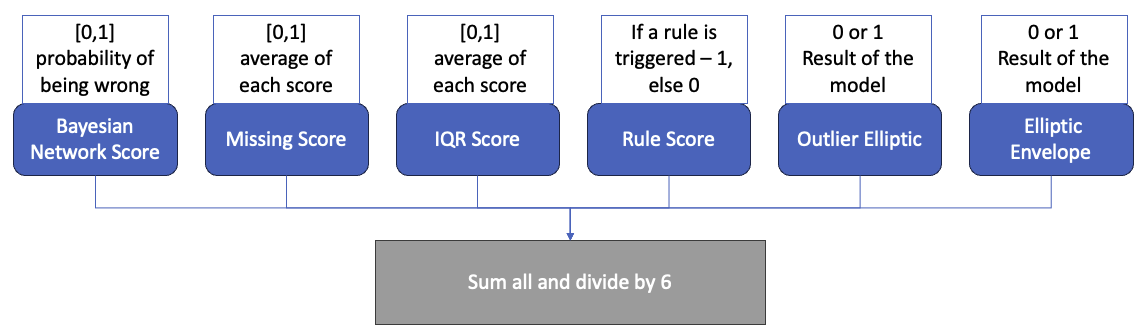
\includegraphics[scale=0.38]{figures/wf-update-dq.png}
    \end{figure}
    %TC:endignore


\subsection{Deployment \& Validation}
The purpose of this model is to serve as an \ac{api} for usage within a healthcare institution and act as a supplementary data quality assessment tool. Although a concrete, vendor-specific information model and health information system were initially used, our goal is to develop a more universal clinical decision support system. This system should be usable across all systems involved in birth and obstetrics departments. Therefore, we constructed it using the \ac{hl7} \ac{fhir} R5 version standard. This approach simplifies the process of API interaction. Rather than utilizing a proprietary model for the data, we based our decision on the use of \ac{fhir} resources: Bundle and Observation. These resources handle the request and response through a customized operation named "\$quality\_check". We intend to publish the profiles of these objects to streamline API access via standardized mechanisms and data models. The model then makes use of the customized operation and of several base resources to construct a \ac{fhir} message, which are: Bundle, MessageHeader, Observation, Device. Observation is where the information about the record is contained, Device contains information about the model, and MessageHeader is used to add information about the request. Finally, the Bundle is used to group all of these resources together. The current version of the profiles can be accessed here \cite{almeidaObstetricsClinicalDecision}.

For validation, we deployed the tool in docker format in a hospital to gather new data. We gathered 3231 new cases and returned a score for quality as exemplified in figure \ref{fig:scores}. Being that the score is from 0 to 1, the average score was 0.23 and \ac{iqr} was 0.03.
As for the clinicians' assessment, we got 4 answers. Figure \ref{fig:clinical} shows the aggregated rankings of the clinicians per record and is ordered by the rank provided by the model.



%TC:ignore
\begin{figure}[htbp]
\centering
\caption{Model score for newly seen data}\label{fig:scores} 
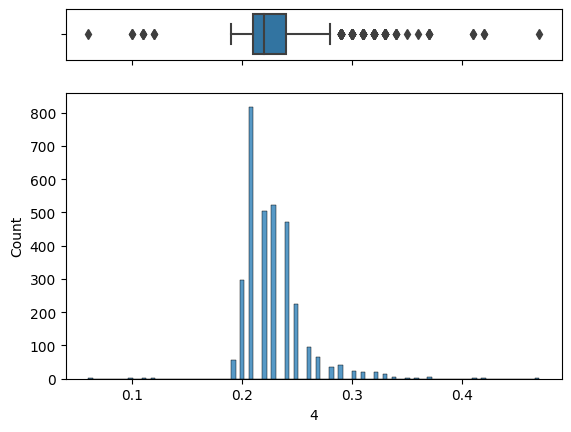
\includegraphics[scale=0.78]{figures/Scoring.png}
\end{figure}
%TC:endignore

%TC:ignore
\begin{figure}[htbp]
\centering
\caption{Comparison of clinical assessment of records with the model. Y is the clinicians' assessment, X is the ranking of the record per the model. Equal numbers on the X mean a tie per the model interpretation. Color is the record ID.}\label{fig:clinical} 
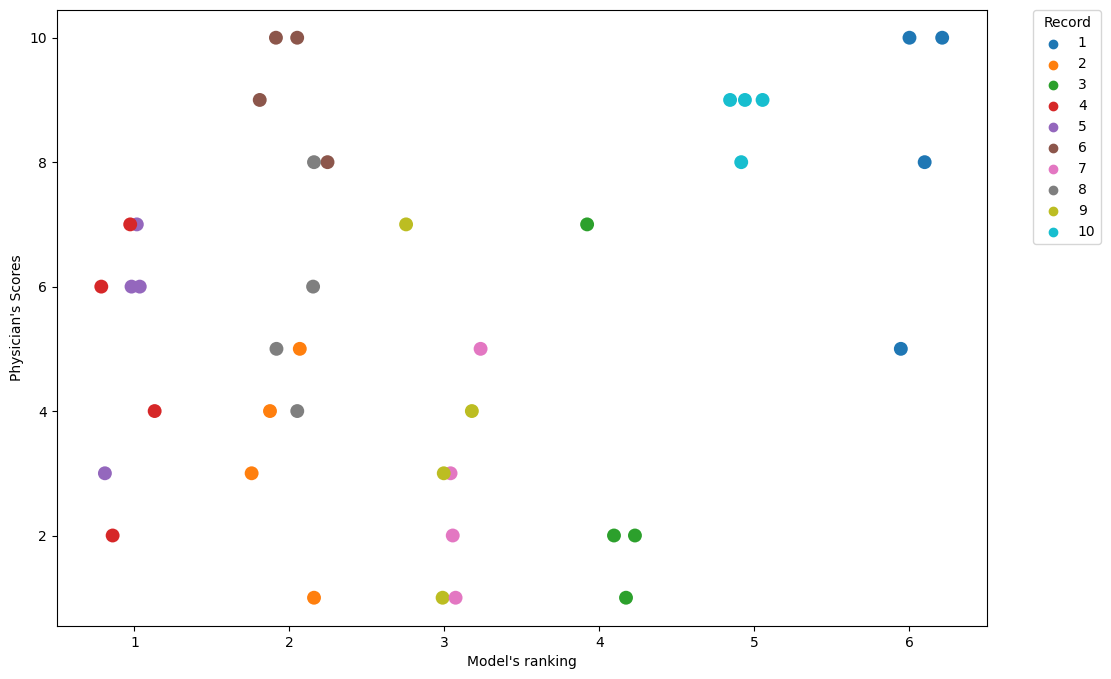
\includegraphics[scale=0.52]{figures/clinical_assessment_dataqual_scatter.png}
\end{figure}
%TC:endignore

The Average Spearman's Rank Correlation Coefficient was 0.04 and the Kendall's Tau was 0.0 with a \textit{\textit{P} value} of 1.

\subsection{Discussion}
% !TeX root = ../../thesis.tex
This work adds several pieces of information to the state of the art of data quality analysis. First we tried to map the output of an automatic assessment tool to the human perception of quality and the issues linked to doing so. Secondly, the fact that we applied \ac{xai} methods such as bayesian networks to leverage the potency of advanced data analysis without compromising interpretability and explainability. Furthermore, a single model was able to reach high performance metrics for almost all variables. Thirdly, the fact that interoperability standard such as \ac{fhir} can be adopted to facilitate the usage and information exchange of such tools. However, there are also shortcoming and challenges to address. The first is that data quality is still an elusive concept since it has a contextual dimension and the quality of the record depends on the usage of the information. For example, data aimed at primary usage and day-to-day healthcare decisions about a patient will have different requirements regarding the importance of some variable or completeness of information very different from data needed to create summary statistics for key performance indicators extraction. Moreover, the data is still very vendor-specific. Even though we used an interoperability standard, the semantic layer, more connected with terminology is still lacking. This is an issue to be addressed in order to improve the interoperability of the standard. Moreover, we do not know how the training done with this data is generalizable to other vendors. One opportunity arises of mapping all of this data to a widely used terminology like SNOMED CT or LOINC. Nevertheless, the usage of FHIR and the fact that the data is mapped to a standard terminology, makes it easier to use the data in other systems and to compare the results with other studies. Furthermore, being available freely and online makes it easier to understand how to map vendor-specific datasets to the model and use it in other contexts. Regarding the model, the usage of explainable methodologies like outlier-tree and transparent models like Bayesian networks are vital for clinical application. Since we use a single model to classify possible errors in the records, the ability to try to show clinicians why that value was tagged is of uttermost importance in order to get feedback and action from humans. From the experience gathered with the study, we believe that a weaker but transparent model could have more impact than better performant but opaque ones. If explainability and interpretability are important for any ML problem, this need only increases when we are dealing with such subjective concepts as data quality.

Regarding the clinical evaluation, we found that asking clinicians to purely assess the quality of a record in an \ac{ehr} is not an easy task. We discovered that for a proper assessment, a context and objective must be defined in order to make the evaluation more objective and manageable. Moreover, the ranking methodology, though very useful for comparison with the model, presents challenges for clinicians who find it difficult to order 10 records when some appear to be of equal quality. This is a very important aspect to consider when designing an evaluation method for data quality. Perhaps a categorical evaluation of yes/no would be more effective than ordering several records. These reasons might explain the great variability between clinicians (figure \ref{fig:clinical-dq}) and between clinicians and the model (Spearman and Kendall tau). Despite that, our preliminary results are promising, demonstrating an \ac{auroc} curve for categorizing bad quality records as high as 88\% and low as 56\%. The highest value was achieved by classifying all record with a mean rank of 4 or above as bad quality and the others as good quality records. However, these results rely on very few samples, so more data and research are needed in this area since it is a very subjective decision, and it should take into account the context and the objective of the evaluation. For example, if the objective is research use, the weights given to each dimension can be a set. On the other hand, if the objective is to use the data for day-to-day clinical decisions, another set of weights could be used. 

For the next steps, a promising research direction would be identifying contexts for applying data quality checks like primary usage, research purposes, and aggregated analysis for decision-making among others. This could enhance targeting those contexts and understanding the importance of each variable for those use cases. Incorporating this approach into the tool to weigh the different variables according to the context would be beneficial.  Finally, gaining access to more data and clinician evaluation of records, although challenging, is important to thoroughly assess the performance of the tool.


\subsection{Conclusion}
% !TeX root = ../../thesis.tex

We believe the work done is already a valuable insight into how to use data quality frameworks and several statistical tools in order to assess EHR data quality in real time. This is a fundamental process not only to guarantee the quality of data for primary usage but also for securing quality for secondary analysis and usage. We believe the fact that we created an interoperable tool that was trained on real obstetrics data from 9 different hospitals and has the ability to provide a single score for a clinical record can help institutions, academics, and EHR vendors implement data quality assessment tools in their own systems and institutions. With the further evaluation of the score and its relationship with clinical usefulness and a further assessment of a threshold for the score for defining a record that would require human attention would be vital to apply this tool in production with high levels of trust and quality.



\begin{savequote}[85mm]
Nothing great in the world was accomplished 
without passion.
\qauthor{Friedrich Hegel}
\end{savequote}

\chapter{Assess health data science  methods with limited data access}\label{chap:goal2}
This section delves into the assessment of health data science methods under the constraints of limited data access, as outlined in sections \ref{subsec:distributed} and \ref{subsec:benchmark}. It emphasizes the importance of developing and evaluating data science techniques that can operate effectively even when direct access to comprehensive datasets is restricted. In section \ref{subsec:distributed}, the focus is on distributed data approaches, which allow for the analysis of health data across multiple locations without the need to centralize the information. This method is crucial for maintaining privacy and security, especially in sensitive health data contexts. Meanwhile, section \ref{subsec:benchmark} discusses benchmarking strategies for these methodologies, providing a framework to evaluate their effectiveness and reliability. These benchmarks are essential to ensure that the methods yield accurate and useful insights, despite the limitations in data accessibility.


\section{Leveraging Distributed systems in healthcare: is it advisable?}\label{subsec:distributed}
This section is based on the paper entitled "Evaluating distributed-learning algorithms on real-world healthcare data". This paper was focused on the fact that access to healthcare data is often laboursome and time-consuming. So we evaluated the distributed paradigm to its gold-standard, the centralized paradigm. We used 9 real-world datasets of obstetrics \acp{ehr} and compared the performance of several \ac{ml} algorithms in both paradigms. We concluded that the distributed paradigm is a valid alternative to the centralized paradigm, with the added benefit of not requiring heavy data sharing.

\subsection{Introduction}
% !TeX root = ../../thesis.tex

%As the use of \ac{ai} is increasing in the healthcare space \cite{deep_learning_increase_health}, increased demand for ethical usage of personal patient data is occurring as well \cite{ehtical_use_ml}. This has been happening both on the governmental side, with several regulations passed to protect citizens' data and personal information (such as \ac{gdpr} in the \ac{eu} \cite{gdpr_article} and \ac{hipaa} in the \ac{us} \cite{hippa}), and on the public side, with an increased concern with continuous data breaches across institutions \cite{abdulrahmanSurveyFederatedLearning2021}. So,  we are now faced with a dilemma on a compromise between what is possible to do with the available data and what should be done regarding patient privacy \cite{swarm_learning}. This is the main reason why health institutions implement burdensome processes and methodologies for sharing patient data, often costing a great deal of time, money, and human resources, seldomly overtaking the ideal time frame for analysing such data.
%Due to these privacy concerns, the traditional method for using data in healthcare is, nowadays, by focusing on data from a single institution in order to predict or infer something regarding those patients; this could be understood as local learning. This approach has some drawbacks, namely data quantity, data quality and possible class imbalance \cite{rajkomarMachineLearningMedicine2019}, never quite raising into its full potential for promoting best healthcare practices
%\cite{federated_healthcare_informatics,usage_ai_healthcare,wangAIHealthState2019} with data sharing between institutions.
%In order to overcome this issue, there are a few, more complex, systems that aggregate data from several institutions, so more robust algorithms could be trained. However, this globally centralised aggregation of data encompasses a very important data breach hazard. 

%This is the setting where distributed learning could create a greater impact. A halfway point between local and centralised learning is where we train several models, one in each institution (or silo), and where the sole information that leaves the premises is a trained model or its metadata. A distributed model is built as the aggregation of all the local models, consequently aiming to create a model similar to one globally trained with all the data in a centralised server. However, the distributed model never contacted with any data, only the local models did. This provides the opportunity to create better models, improve data protection, reduce training time and cost and provide better scaling capabilities  \cite{jatainContemplativePerspectiveFederated2021}.

%including federated-learning approaches, where a central system orchestrates the operation \cite{federated_learning_intro} or a swarm/peer-to-peer framework where silos communicate with each other. However,
%There are already some implementations of distributed systems in the healthcare space, but we lack a robust understanding of how these models behave with real data, when compared with the classical models built with all the aggregated data. Additionally, the main issues regarding the development and implementation of such systems in healthcare are still elusive.
%So we aim to understand how distributed mechanisms behave compared to using all data in the healthcare space and if they are a suitable replacement for traditional machine-learning pipelines. The contributions of this paper are:
%\begin{myitemize}
%    \item Understand how to address the lack of data quality of real-world data regarding distributed model creation;
%    \item Evaluate a distributed model against its local counterparts;
%    \item Measure the prediction performance difference between a distributed model and a centralised one;
%    \item Identify the capabilities of a distributed model to track population changes on the local datasets;
%    \item Open a research path for using distributed models to predict several target variables in obstetrics clinical research.
%\end{myitemize}


As the use of \ac{ai} is increasing in the healthcare space \cite{deep_learning_increase_health}, increased demand for ethical usage of personal patient data is occurring as well \cite{ehtical_use_ml}. This has been happening both on the governmental side, with several regulations passed to protect citizens' data and personal information (such as \ac{gdpr} in the \ac{eu} \cite{gdpr_article} and \ac{hipaa} in the \ac{us} \cite{hippa}), and on the public side, with an increased concern with continuous data breaches across institutions \cite{abdulrahmanSurveyFederatedLearning2021}. So,  we are now faced with a dilemma on a compromise between what is possible to do with the available data and what should be done regarding patient privacy \cite{swarm_learning}. This is the main reason why health institutions implement burdensome processes and methodologies for sharing patient data, often costing a great deal of time, money, and human resources, seldomly overtaking the ideal time frame for analysing such data.
Due to these privacy concerns, the traditional method for using data in healthcare is, nowadays, by focusing on data from a single institution in order to predict or infer something regarding those patients; this could be understood as local learning. This approach has some drawbacks, namely data quantity, data quality and possible class imbalance \cite{rajkomarMachineLearningMedicine2019}, never quite raising into its full potential for promoting the best healthcare practices
\cite{federated_healthcare_informatics,usage_ai_healthcare,wangAIHealthState2019} with data sharing between institutions.
In order to overcome this issue, there are a few, more complex, systems that consolidate data from several institutions, so more robust algorithms could be trained. However, this globally centralised consolidation of data encompasses a very important data breach hazard. 

This is the setting where distributed learning could create a greater impact. A halfway point between local and centralised learning is where we train several models, one in each institution (or silo), and where the sole information that leaves the premises is a trained model or its metadata. A distributed model is built as the aggregation of all the local models, consequently aiming to create a model similar to one globally trained with all the data in a centralised server. However, the distributed model never contacted with any data, only the local models did. This provides the opportunity to create better models, improve data protection, reduce training time and cost and provide better scaling capabilities  \cite{jatainContemplativePerspectiveFederated2021}.

%including federated-learning approaches, where a central system orchestrates the operation \cite{federated_learning_intro} or a swarm/peer-to-peer framework where silos communicate with each other. However,
%There are already some implementations of distributed systems in the healthcare space, but we lack a robust understanding of how these models behave with real data, when compared with the classical models built with all the aggregated data. So we aim to understand how distributed mechanisms behave compared to using all data in the healthcare space and if they are a suitable replacement for traditional machine-learning pipelines. The contributions of this paper are:

While numerous multi-institutional initiatives have successfully established integrated data repositories for healthcare research, there remains an incomplete understanding of the performance and scalability of distributed systems when directly compared to traditional, centralised models. Specifically, the nuanced behaviours of these distributed frameworks under real-world data conditions—contrasted against classical models that utilize consolidated data—have yet to be fully delineated. This paper aims to critically evaluate the efficacy and suitability of distributed mechanisms within the healthcare domain, assessing their potential as viable alternatives to conventional machine-learning pipelines. The contributions of this paper include:

\begin{myitemize}
    \item Evaluate a distributed model against its local counterparts;
    \item Measure the prediction performance difference between a distributed model and a centralised one;
%    \item Identify the capabilities of a distributed model to track population changes on the local datasets;
    %\item Understand how to address the lack of data quality of real-world data regarding distributed model creation;

  %  \item Open a research path for using distributed models to predict several target variables in obstetrics clinical research.
\end{myitemize}

\subsection{Theoretical background and Related Work}
Distributed learning \cite{distributed} can be understood as training several models in a different setting and then aggregating them as a whole. There are two main branches of these approaches, distinguishable by the existence of a central orchestrator server: federated learning where such an entity exists, and peer-to-peer (or swarm) \cite{swarm_learning} learning where it does not. 
Even though distributed learning has been receiving a lot of attention recently, only some of its concepts have been focused on, mainly distributed-deep learning with a federated learning approach \cite{xuFederatedLearningHealthcare2021,leeFederatedLearningClinical2020}. These methods use the strength of neural networks and several algorithms like federated averaging to create distributed models capable of handling complex data like text, sound, or image \cite{prayitnoSystematicReviewFederated2021}. However, considering that there are great amounts of information, especially in healthcare, stored as tabular data \cite{alvarezsanchezTAQIHToolTabular2019,dimartinoExplainableAIClinical2022,payrovnaziriExplainableArtificialIntelligence2020} and that neural networks are often not the best tool for such data structures \cite{borisovDeepNeuralNetworks2022a}, there is a lack of knowledge in the traditional machine learning techniques in a distributed manner.
%Federated Learning was introduced in 2016 \cite{konecny_federated_2016,mcmahanFederatedLearningDeep2016} and it was called federated since "the learning task is solved by a loose federation of participating devices (which we refer to as clients) which are coordinated by a central server" \cite{konecny_federated_2016}. Federated learning has two main architectures: a) horizontal and b) vertical  \cite{yangFederatedMachineLearning2019b}. 
%Horizontal refers to having the same features in all silos, but different populations in each silo. Vertical refers to having different features across silos for the same population. Then we have other approaches that expand the concept of federated learning with previous machine learning and deep learning methodologies such as transfer learning, reinforcement learning \cite{liuSystematicLiteratureReview2020} and quantum machine-learning \cite{quantum-fed-ml}. 
%Federated learning can also be classified by the information flow. Model data can be shared only with the main central server, as in more traditional methods, but also being incremental, sharing data model sequentially between silos, with central server orchestration \cite{cyclic_distribution}. 

Nevertheless, there have been some health-related  distributed machine-learning projects successfully implemented, such as euroCAT  \cite{eurocat} which implemented an infrastructure across five clinics in three countries. \ac{svm} models were used to learn from the data distributed across the five clinics. Each clinic has a connector to the outside where only the model's parameters are passed to the central server which acts as a master deployer regarding the model training with the radiation oncology data.
Also, ukCAT \cite{ukcat} did similar work, with an added centralised database in the middle, but the training being done with a decentralized system.
%Other methods and approaches have been also evaluated such as the work of Brisimi et. al. \cite{brisimi_federated_2018}  for predicting hospitalisations or deep learning methods oriented to analysing medical imaging \cite{chang_distributed_2018}, evaluating histological samples \cite{pathology-fl} and finally, some preprints showing the impact of federated learning regarding COVID-19 prediction \cite{vaid_federated_2020}. For a sound review please redirect to Zerka et al. \cite{zerkaSystematicReviewPrivacyPreserving2020a}

Finally, a few works have explored the evaluation of models in a distributed manner, for example, comparing  centralised machine learning, distributed machine learning and federated learning on MNIST dataset \cite{performance_evaluation_1}. Also, works that evaluate federated learning on MNIST, MIMIC-III and PhysioNet ECG datasets, but not in comparison with other methods  \cite{performance_evaluation_2}. The work by Tuladhar and colleagues \cite{distributed} uses healthcare images and/or public and curated datasets.
As far as we know, this is the first time a distributed machine learning evaluation is done with real-world clinical data from several different data sources.
\subsection{Materials}
Clinical data was gathered from nine different Portuguese hospitals regarding obstetric information, pertaining to admissions from 2019 to 2020. This originated nine different files representing different sets of patients but with the same features associated to them. The software for collecting data was the same in every institution (although different versions existed across hospitals) - ObsCare. The data columns are the same in every hospital's database. Each hospital was considered a silo and summary statistics of the different silos are reported in the tables \ref{tab:distributed_materials_1} and \ref{tab:distributed_materials_2}. The data dictionary is in appendix \ref{appendix:data_dict}.
%TC:ignore

{\small
\begin{table}[!ht]

\caption[Silos overview.]{\label{tab:distributed_materials_1}Silos overview. categorical columns have a snippet of the most used category and a percentage. Continuous variables have a mean and standard deviation. Abbreviation meaning in the appendix. The last row is the number of patients. * columns were used as target.}

\centering
% !TeX root = ../../thesis.tex
\newcolumntype{L}{>{\scriptsize}l}  % "small" can be changed to "scriptsize" or "footnotesize" for even smaller text

\begin{tabular}{LLLLLLL}
   \toprule
      Variable &               Silo 1 &               Silo 2 &               Silo 3 &               Silo 4 &               Silo 5 &                Total \\
   \midrule
   \hspace*{2mm} N (total) &              8039 &                 8566 &                 4989 &                 2364 &                18177 &                80874 \\
   
   \textbf{Actual Type of Delivery C (\%)}& 10 (52.6) & 3 (51.6) & 3 (57.8) & 3 (61.8) & 9 (61.5) & 11 (52.9) \\
   
   Bishop Score C (\%)&  15 (98.5) & 15 (78.8) & 13 (97.4) & 16 (86.4) & 15 (97.4) & 16 (95.3) \\
   
   \textbf{Blood Group C (\%)}& 9 (39.9) & 10 (39.9) & 9 (39.3) & 11 (37.9) & 10 (40.9) & 14 (40.5) \\
   
   \textbf{Body Mass Index $\mu (\sigma)$ } & 25.2 (8.6) & 25.2 (6.2) & 25.0 (5.3) & 25.0 (8.9) & 24.9 (7.8) & 25.1 (7.0) \\
   
   Cervical Consistency C (\%) & 4 (98.6) & 4 (83.4) & 4 (99.3) & 4 (87.4) & 4 (97.5) & 4 (96.5) \\
   
   Cervical Position C (\%)&  4 (98.6) & 4 (83.3) & 4 (99.3) & 4 (87.5) & 4 (97.6) & 4 (96.6) \\
   
   \textbf{Delivery Type C (\%)}& 6 (43.4) & 6 (53.5) & 5 (44.4) & 7 (52.2) & 7 (49.3) & 8 (51.3) \\
   
   Dilatation C (\%)&5 (98.5) & 5 (83.1) & 5 (99.3) & 5 (87.2) & 5 (97.5) & 5 (96.5) \\
   
   Effacement C (\%)& 5 (98.6) & 5 (83.2) & 5 (99.3) & 5 (87.2) & 5 (97.5) & 5 (96.5) \\
   
   Fetal Station  C (\%)&  5 (98.6) & 5 (83.3) & 5 (99.3) & 5 (87.9) & 5 (97.5) & 5 (96.6) \\
   
   \textbf{Followed physician C (\%)} & 3 (99.2) & 4 (92.2) & 3 (99.1) & 3 (94.3) & 3 (99.0) & 4 (97.9) \\
   
   \textbf{\begin{minipage}{3.8cm}\setstretch{0.65}Followed physician hospital delivery C (\%)\vspace{1mm}\end{minipage}}&  2 (87.6) & 2 (75.8) & 2 (81.4) & 2 (52.2) & 2 (71.0) & 2 (69.0) \\
   
   \textbf{\begin{minipage}{3.8cm}\setstretch{0.65}Followed physician primary care C (\%)\vspace{1mm}\end{minipage}}&  2 (61.3) & 2 (52.8) & 2 (78.1) & 2 (50.4) & 2 (70.4) & 2 (67.6) \\
   
   \begin{minipage}{3.8cm}\setstretch{0.65}Followed physician private clinic C (\%)\vspace{1mm}\end{minipage}&  2 (81.8) & 2 (85.0) & 2 (80.6) & 2 (78.8) & 2 (73.3) & 2 (75.8) \\
   
   Gestational Diabetes C (\%)&2 (87.7) & 2 (90.0) & 2 (90.2) & 2 (90.8) & 2 (89.8) & 2 (89.5) \\
   
   
   Induced Delivery  C (\%)& 2 (97.8) & 2 (83.9) & 2 (93.3) & 2 (91.9) & 2 (98.5) & 2 (92.5) \\
   
   \textbf{Mother Age $\mu (\sigma)$ } & 31.1 (5.7) & 30.7 (5.6) & 31.1 (5.9) & 31.1 (6.3) & 31.3 (5.6) & 31.1 (5.6) \\
   
   
   \begin{minipage}{3.9cm}\setstretch{0.65}Nr Deliveries forceps C (\%)\end{minipage} & 4 (99.2) & 3 (83.3) & 4 (94.3) & 4 (95.8) & 3 (60.1) & 5 (82.6) \\
   
   
   \begin{minipage}{3.9cm}\setstretch{0.65}Nr Deliveries no assistance C (\%)\vspace{1mm}\end{minipage} & 10 (74.7) & 9 (60.3) & 9 (74.9) & 9 (67.3) & 11 (45.4) & 12 (60.3) \\
   
   \begin{minipage}{3.9cm}\setstretch{0.65}Nr Deliveries vacuum C (\%)\vspace{1mm}\end{minipage} &  5 (90.4) & 4 (79.9) & 4 (89.0) & 4 (93.1) & 5 (55.3) & 5 (77.4) \\
   
   Nr of C-sections C (\%) & 6 (87.9) & 6 (72.6) & 5 (86.1) & 5 (89.5) & 6 (62.1) & 6 (74.6) \\
   
   \textbf{Nr of Pregnancies C (\%)} &  11 (40.9) & 11 (43.1) & 13 (39.1) & 12 (38.7) & 16 (42.8) & 19 (42.1) \\
   
   \textbf{Nr of born babies C (\%)} & 10 (44.8) & 10 (41.4) & 10 (36.9) & 10 (42.0) & 12 (35.3) & 12 (38.8) \\
   
   \textbf{Nr of consultations $\mu (\sigma)$ } &  7.3 (4.7) & 7.0 (6.4) & 6.4 (3.9) & 5.5 (3.6) & 10.5 (5.1) & 8.4 (5.1) \\
   
   Pelvis Adequacy C (\%) &4 (95.4) & 4 (77.7) & 4 (90.1) & 3 (96.9) & 4 (81.2) & 4 (82.6) \\
   
   \textbf{Position Admission C (\%)}  &  5 (88.5) & 6 (78.0) & 6 (51.8) & 3 (95.9) & 6 (71.3) & 7 (73.1) \\
   
   
   \textbf{Position on Delivery C (\%)} &5 (91.5) & 5 (94.4) & 5 (94.7) & 5 (95.5) & 5 (94.3) & 5 (93.9) \\
   
   \textbf{Pregnancy Type C (\%)} &  7 (62.1) & 7 (90.5) & 7 (85.4) & 7 (63.0) & 7 (89.2) & 7 (85.4) \\
   
   \textbf{Robson Group C (\%)} & 11 (22.4) & 11 (20.1) & 10 (23.8) & 10 (80.5) & 11 (27.7) & 11 (24.4) \\
   
   \begin{minipage}{3.7cm}\setstretch{0.65}Rupture amniotic pocket before delivery C (\%)\end{minipage} &  2 (91.1) & 2 (93.6) & 2 (89.3) & 2 (91.6) & 2 (84.6) & 2 (88.5) \\
   
   Smoker C (\%) & 2 (84.4) & 2 (85.2) & 2 (87.2) & 2 (89.7) & 2 (87.9) & 2 (88.1) \\
   
   \textbf{Spontaneous Delivery C (\%)} &  2 (70.3) & 2 (74.7) & 2 (64.8) & 2 (64.3) & 2 (59.7) & 2 (64.9) \\
   
   \textbf{Weeks on Admission C (\%)} &    38.1 (3.5) &    38.8 (2.2) &    38.9 (1.6) &    38.8 (2.4) &    38.6 (2.1) &    38.7 (2.2) \\
   
   
   \textbf{Weeks on Delivery $\mu (\sigma)$ } &    38.5 (2.8) &    38.9 (2.0) &    39.1 (1.7) &    39.0 (2.3) &    38.9 (2.0) &    38.9 (2.0) \\
   
   Weight on Admission $\mu (\sigma)$  &   81.4 (14.9) &   79.5 (14.5) &   78.0 (15.2) &   79.6 (16.3) &   78.3 (14.2) &   78.8 (14.5) \\
   
   
   \textbf{\begin{minipage}{3.3cm}\setstretch{0.65}Weight start  of pregnancy $\mu (\sigma)$ \vspace{1mm}\end{minipage}} &   66.4 (14.4) &   66.1 (13.5) &   65.5 (14.1) &   65.5 (14.1) &   65.5 (14.4) &   66.0 (14.1) \\
   \bottomrule
   \end{tabular}
   
   
\end{table}
}
\newpage

{\small
\begin{table}[!ht]

\caption[Silos overview part 2.]{\label{tab:distributed_materials_2}Silos overview part 2. categorical columns have a snippet of the most used category and a percentage. Continuous variables have a mean and standard deviation. Abbreviation meaning in the appendix. The last row is the number of patients. * columns were used as target.}
\centering
% !TeX root = ../../thesis.tex

\begin{tabular}{llllll}
   \toprule
   Variable &               Silo 6 &               Silo 7 &               Silo 8 &               Silo 9 &                Agrr. \\
   \midrule
   
   \hspace*{2mm}  N (total) &                12002 &                 8258 &                 6693 &                11786 &                80874 \\
   
   \textbf{Actual Type of Delivery C (\%)} & 10 (63.8) & 0 (100) & 10 (50.1) & 9 (64.6) & 11 (52.9) \\
   Bishop Score C (\%) & 14 (99.3) & 15 (97.9) & 14 (99.2) & 15 (95.0) & 16 (95.3) \\
   \textbf{Blood Group C (\%)} & 13 (41.6) & 10 (39.2) & 10 (40.1) & 10 (41.7) & 14 (40.4) \\
   \textbf{Body Mass Index $\mu (\sigma)$ } & 24.9 (5.1) & 24.9 (7.0) & 24.8 (8.0) & 25.7 (5.6) & 25.1 (7.0) \\
   Cervical Consistency C (\%)  & 4 (99.5) & 4 (99.7) & 4 (99.5) & 4 (96.9) & 4 (96.5) \\
   Cervical Position C (\%) & 4 (99.5) & 4 (99.7) & 4 (99.5) & 4 (96.9) & 4 (96.5) \\
   \textbf{Delivery Type C (\%)} & 6 (54.3) & 5 (52.1) & 5 (47.8) & 5 (59.0) & 8 (51.3) \\
   Dilatation C (\%) & 5 (99.5) & 5 (99.7) & 5 (99.5) & 5 (96.9) & 5 (96.5) \\
   Effacement C (\%)  & 5 (99.5) & 5 (99.7) & 5 (99.5) & 5 (96.9) & 5 (96.5) \\
   Fetal Station C (\%) & 5 (99.5) & 5 (99.7) & 5 (99.5) & 5 (96.9) & 5 (96.6) \\
   \textbf{Followed physician C (\%)} & 3 (96.9) & 3 (99.4) & 3 (97.8) & 3 (99.2) & 4 (97.8) \\
   \textbf{\begin{minipage}{3.8cm}\setstretch{0.65}Followed physician hospital delivery C (\%)\vspace{1mm}\end{minipage}}& 2 (62.1) & 2 (63.2) & 2 (69.4) & 2 (83.1) & 2 (69.0) \\
   \textbf{\begin{minipage}{3.8cm}\setstretch{0.65}Followed physician primary care C (\%)\vspace{1mm}\end{minipage}} & 2 (53.1) & 2 (86.7) & 2 (63.1) & 2 (87.3) & 2 (67.6) \\
   \begin{minipage}{3.9cm}\setstretch{0.65}Followed physician private clinic C (\%)\vspace{1mm}\end{minipage} & 2 (68.2) & 2 (73.5) & 2 (71.0) & 2 (78.1) & 2 (75.8) \\
   Gestational Diabetes C (\%)  & 2 (92.2) & 2 (88.2) & 2 (89.9) & 2 (86.8) & 2 (89.5) \\
   Induced Delivery C (\%) & 2 (91.9) & 2 (85.9) & 2 (87.4) & 2 (93.9) & 2 (92.5) \\
   \textbf{Mother Age $\mu (\sigma)$ }  & 31.3 (5.2) & 31.4 (5.4) & 31.5 (5.6) & 30.1 (5.6) & 31.1 (5.6) \\
   
   \begin{minipage}{3.9cm}\setstretch{0.65}Nr Deliveries forceps C (\%)\vspace{1mm}\end{minipage} & 4 (82.0) & 4 (86.0) & 3 (94.0) & 4 (89.3) & 5 (82.6) \\
   \begin{minipage}{3.9cm}\setstretch{0.65}Nr Deliveries no assistance C (\%)\vspace{1mm}\end{minipage}  & 8 (58.8) & 9 (61.2) & 10 (68.9) & 9 (61.5) & 12 (60.3) \\
   \begin{minipage}{3.9cm}\setstretch{0.65}Nr Deliveries vacuum C (\%)\vspace{1mm}\end{minipage}& 4 (78.9) & 4 (81.6) & 4 (88.0) & 5 (82.3) & 5 (77.4) \\
   Nr of C-sections C (\%) & 6 (69.1) & 6 (74.5) & 5 (85.5) & 6 (77.8) & 6 (74.6) \\
   \textbf{Nr of Pregnancies C (\%)} & 13 (44.2) & 9 (42.9) & 11 (42.0) & 13 (40.2) & 19 (42.1) \\
   \textbf{Nr of born babies C (\%)} & 9 (38.4) & 9 (42.6) & 10 (41.2) & 10 (43.2) & 12 (38.8) \\
   \textbf{Nr of consultations $\mu (\sigma)$ } & 6.8 (4.0) & 7.7 (3.2) & 9.3 (4.5) & 8.9 (5.5) & 8.4 (5.1) \\
   Pelvis Adequacy  C (\%)  & 4 (89.6) & 4 (52.9) & 3 (93.1) & 4 (81.5) & 4 (82.6) \\
   \textbf{Position Admission C (\%)} & 6 (84.5) & 7 (61.3) & 5 (89.2) & 4 (74.2) & 7 (73.1) \\
   \textbf{Position on Delivery C (\%)} & 5 (93.0) & 5 (93.6) & 5 (94.8) & 5 (94.2) & 5 (93.9) \\
   
   \textbf{Pregnancy Type C (\%)} & 7 (88.0) & 7 (85.4) & 7 (86.0) & 7 (92.9) & 7 (85.4) \\
   \textbf{Robson Group C (\%)}& 11 (27.2) & 11 (24.7) & 11 (21.4) & 11 (26.7) & 11 (24.4) \\
   \begin{minipage}{3.7cm}\setstretch{0.65}Rupture amniotic pocket before delivery C (\%)\vspace{1mm}\end{minipage} & 2 (85.0) & 2 (84.4) & 2 (89.9) & 2 (93.8) & 2 (88.5) \\
   Smoker C (\%) & 2 (91.0) & 2 (90.7) & 2 (85.5) & 2 (89.9) & 2 (88.1) \\
   \textbf{Spontaneous Delivery C (\%)} & 2 (64.9) & 2 (64.0) & 2 (64.7) & 2 (62.9) & 2 (64.9) \\
   Weeks on Admission $\mu (\sigma)$ & 38.7 (1.8) & 39.0 (2.0) & 38.6 (2.1) & 38.8 (1.9) & 38.7 (2.2) \\
   \textbf{Weeks on Delivery $\mu (\sigma)$ }  & 38.8 (1.8) & 39.2 (1.7) & 38.7 (2.0) & 39.0 (1.6) & 38.9 (2.0) \\
   \textbf{Weeks on Admission $\mu (\sigma)$ } & 77.7 (13.4) & 79.2 (14.7) & 76.7 (13.0) & 83.1 (15.2) & 78.8 (14.5) \\
   \textbf{\begin{minipage}{3.3cm}\setstretch{0.65}Weight start of pregnancy $\mu (\sigma)$ \vspace{1mm}\end{minipage}}  & 65.6 (13.5) & 66.0 (13.7) & 65.6 (14.1) & 67.4 (14.6) & 66.0 (14.1) \\
   
   
   
   \bottomrule
   \end{tabular}
   

\end{table}
}
%TC:endignore

\subsection{Methods}
% !TeX root = ../../thesis.tex

The section will cover the steps we took for evaluating the models. We first addressed the preprocessing of the data, then the training of the models and finally the evaluation of the models. The evaluation was done by comparing the performance of the distributed model with the local and centralised models. The performance was measured by the AUROC, AUPRC, RMSE and MAE. The results were then compared using a 2-sample T-test.
\subsubsection{Preprocessing}

The initial dataset underwent preprocessing by eliminating attributes that were missing more than 90\% of their data across all storage units (or silo). We standardized the representation of missing values, which varied widely, including representations such as "-1" "missing" or simply blank spaces. For imputation, we utilized the mean for continuous variables (calculated within site) and introduced a special category (NULLIMP) for categorical variables. We converted all categories into numerical values based on a predefined mapping that covered all potential categories across the datasets. Although this approach introduces an ordinal relationship and potential bias is created among features, we disregarded this concern because the methodology was uniformly applied across all datasets intended for training local, distributed and centralised. These preprocessing tasks were executed once for each dataset and silo.

However, in the context of training classification models, it is crucial that all classes of the target variable are known at the time of training and are represented in each split of the cross-validation process. To address this, we employed SMOTE \cite{smote} to up-sampled low-frequency target classes. We established a threshold of n$<$25 for low-frequency variables to ensure that each cross-validation split contained at least two instances of the class—although a minimum of 10 instances (10 splits) might suffice, we opted for 25 to mitigate potential distribution issues and have at least two examples of the class in each split. Additionally, we created dummy rows for missing target classes by imputing the mean for continuous variables and the mode for categorical variables (calculated within site). The necessity for up-sampling and missing variable creation was evaluated and applied as needed for each training session and for each target, considering that each session's split could result in a training set lacking instances of low-frequency classes.

All procedures were coded in python 3.9.7 with the usage of the scikit-learn library \cite{scikit-learn} and mlxtend library \cite{mlxtend}.


\subsubsection{Model Training}
To avoid pitfalls of inductive bias from a certain learning strategy, we learned six different models (i) Decision Trees, (ii) Bayesian methods, (iii) a logistic regression model with Stochastic Gradient Descent, (iv) K-nearest neighbours, (v) AdaBoost and (vi) Multi-layer Perceptron. The decision was to create diversity in the models used, in order to assess if the training methodology could have an impact on distributed model creation.
The distributed model was an ensemble of models from each silo on a weighted soft-voting basis. The weights were defined by weighted averages of the scores each model obtained in the training set. Then the final result is obtained by creating a weighted average of the class predictions for classification and a weighted average for regression. A model like this can be implemented with peer-to-peer or federated approaches.
Nineteen features were used as target outcomes. These features were selected by filtering by the percentage of null values (below 50\%). This choice was related to maintaining a equilibrium between having a wide range of variables to test how the target variables affects the outcome and having target variables that did go through an harsh imputation mechanism. For categorical outcomes, thirteen were selected (AA - Position Admission; ANP - Position on Delivery; AGESTA - Nr of Pregnancies; APARA - Nr of born babies; GS - Blood Group; GR - Robson Group; TG -Pregnancy Type; TP - Delivery Type; TPEE - Spontaneous Delivery; TPNP - Actual Type of Delivery; V - Followed physician; VCS - Followed physician primary care; VNH - Followed physician hospital delivery;). For continuous variables, six were selected (IA - Mother Age; IGA - Weeks on Admission; IMC - BMI; NRCPN - Nr of consultations; PI - Weight start of pregnancy; SGP - Weeks on Delivery;). Details can be seen in tables \ref{tab:1} and \ref{tab:1.2}.
Local models were built with each silo's data. The centralised model was trained with a training dataset from all the silos combined. 


%TC:ignore
\subsubsection{Model Performance Evaluation}

All models were built for a certain outcome variable with a repeated cross-validation (2 times and 10 splits each) and then compared, over 10 stochastic runs, with evaluation being performed on a test set held out from each silo. By performing cross-validation twice, we aimed to generate a more robust estimation of the model’s performance metrics by averaging the results over two separate runs, each partitioning the data differently. This approach is particularly useful in scenarios where data is limited or highly variable, as it provides a clearer insight into the model's expected performance in unseen data scenarios. The metrics used for classification models were Weighted Area Under the Receiver Operating Characteristic Curve (AUROC) computed as One-versus-Rest, Weighted Area Under the Precision-Recall Curve (AUPRC). The metrics for regression models were Root Mean Squared Error (RMSE) and Mean Absolute Error (MAE). The algorithm is shown in the algorithm \ref{alg:1}. This rendered over 1000 different combinations. When a variable was used as outcome to predict, all others were used as predictors.




\begin{algorithm}[hbtp]
\caption{Creation and evaluation of the 3 different models. We first preprocessed data. Then for each target, we created a distributed and centralised model. Then, over 10 repetitions per silo, we created a new train and test set and local model and tested the centralised, distributed and local on this test set.}
\label{alg:1}
Pre-process all silos (null standardization, imputation, encoding)\;
\For {target in target list}{ 
  \For{n in 10 repetitions}{

\For {silo in imputed silos}{
Train-Test Split (80:20)\;
 check for low frequency or nonexistent labels in train set \;
 train local model with hyper-parameter tuning with 2x10 repeated CV \;
 define weights based on scores in the train set (weighted average for predicting the value) for the distributed model\;

  }

  Create distributed (ensemble of all models) model with weights\;
  predict local on the test set\;
  predict distributed on the test set\;
\vspace{3mm}


Create a centralised model with all the data with a 2x10 repeated CV \;
Test the centralised model on the test set\;
}}



 \end{algorithm}
%TC:endignore

After all the data was collected, we used the standard independent 2-sample T-test to check if the differences were significant with a $\alpha$ of 0.05. First, we compared the overall performance of the distributed model vs their centralised and local counterpart.  We also compared every distributed model per algorithm and sequentially the centralised and correspondent local model across all algorithms and repetitions and outcome variables with 2-sample T-test as well.



\subsection{Results}
% !TeX root = ../../thesis.tex

Table \ref{tab:allvsall} shows the aggregated metrics for AUROC, AUPRC, RMSE and MAE for distributed, centralised and local models predicting capabilities on each silo. The data refers to the mean of the metric values for all columns tested as targets for all methods and all silos. We also calculated the 95\% confidence interval for each model (local and distributed per silo) in order to assess how well the distributed model would work as opposed to the local one per silo. We also calculated the p Value for the means of the distributed vs centralised and distributed vs local.
%TC:ignore
%\setlength{\tabcolsep}{7pt} % Default value: 6pt
%\renewcommand{\arraystretch}{1.3} % Default value: 1

\begin{table}[h!] 
 \setlength{\tabcolsep}{7pt} % Default value: 6pt 
 \renewcommand{\arraystretch}{1.3} % Default value: 1
  \captionsetup{justification=centering} 
\centering
\caption[Metrics for centralised model, distributed model and local model]{Comparison of the distributed model with the centralised model and with the local model (Mean for all model and all columns). 2-sample T-test for the means was used as hypothesis test. Bold for \textit{P} value below 0.05. AUPRC and AUROC for categorical target variable and RMSE and MAE for continuous target variable.}

\label{tab:allvsall}
\begin{tabular}{llcccc}
\toprule
 &  & M & SD & 95\% CI & \textit{P}  \\
\midrule
\multirow{3}{*}{AUPRC}
 & distributed & 0.691 & 0.216 & (0.686, 0.696) & - \\
  & centralised & 0.706 & 0.225 & (0.701, 0.711) & \bfseries 1.10e-17 \\
 & local & 0.659 & 0.220 & (0.654, 0.665) & \bfseries 4.71e-05 \\
 \hline

\multirow{3}{*}{AUROC} 
 & distributed & 0.723 & 0.182 & (0.718, 0.727) & - \\
 & centralised & 0.729 & 0.180 & (0.725, 0.734) & \bfseries 2.98e-26 \\
 & local & 0.692 & 0.164 & (0.688, 0.695) & \bfseries 2.48e-02 \\

\hline

\multirow{3}{*}{MAE} 
 & distributed & 2.370 & 1.608 & (2.315, 2.425) & - \\
 & centralised & 2.365 & 1.923 & (2.298, 2.431) & \bfseries 2.23e-04 \\
 & local & 2.527 & 1.799 & (2.465, 2.589) & 9.01e-01 \\

\hline

\multirow{3}{*}{RMSE} 
 & distributed & 21.171 & 46.078 & (19.584, 22.757) & - \\
 & centralised & 19.839 & 28.645 & (18.853, 20.826) & \bfseries 2.92e-02 \\
 & local & 23.771 & 49.776 & (22.057, 25.485) & 1.63e-01 \\
\hline
\end{tabular}
\end{table}





%TC:endignore

Figure \ref{fig:heatmap-cat} shows the AUROC of each algorithm and silo on the Y axis and target variable and type of model on the X. The color bar refers to the value of the AUROC. Blue being lower values and red bigger values. The same type of graph was created for regression, where the Figure \ref{fig:heatmpa-int} shows the MAE for each silo and algorithm and target variable and type of model. 


%TC:ignore

\begin{figure}[h!]
\centering
\captionsetup{justification=centering}

\caption[Heatmap of classification algorithm and silo vs Target variable and model type.]{Heatmap of classification algorithm and silo vs Target variable and model type. Value is the AUROC mean of all 10 experiments. Y axis is the algorithm and silo. X axis is Target variable and Method. AA - Position Admission; ANP - Position on Delivery; AGESTA - Nr of Pregnancies; APARA - Nr of born babies; GS - Blood Group; GR - Robson Group; TG -Pregnancy Type; TP - Delivery Type; TPEE - Spontaneous Delivery; TPNP - Actual Type of Delivery; V - Followed physician; VCS - Followed physician primary care; VNH - Followed physician hospital delivery;}\label{fig:heatmap-cat} 
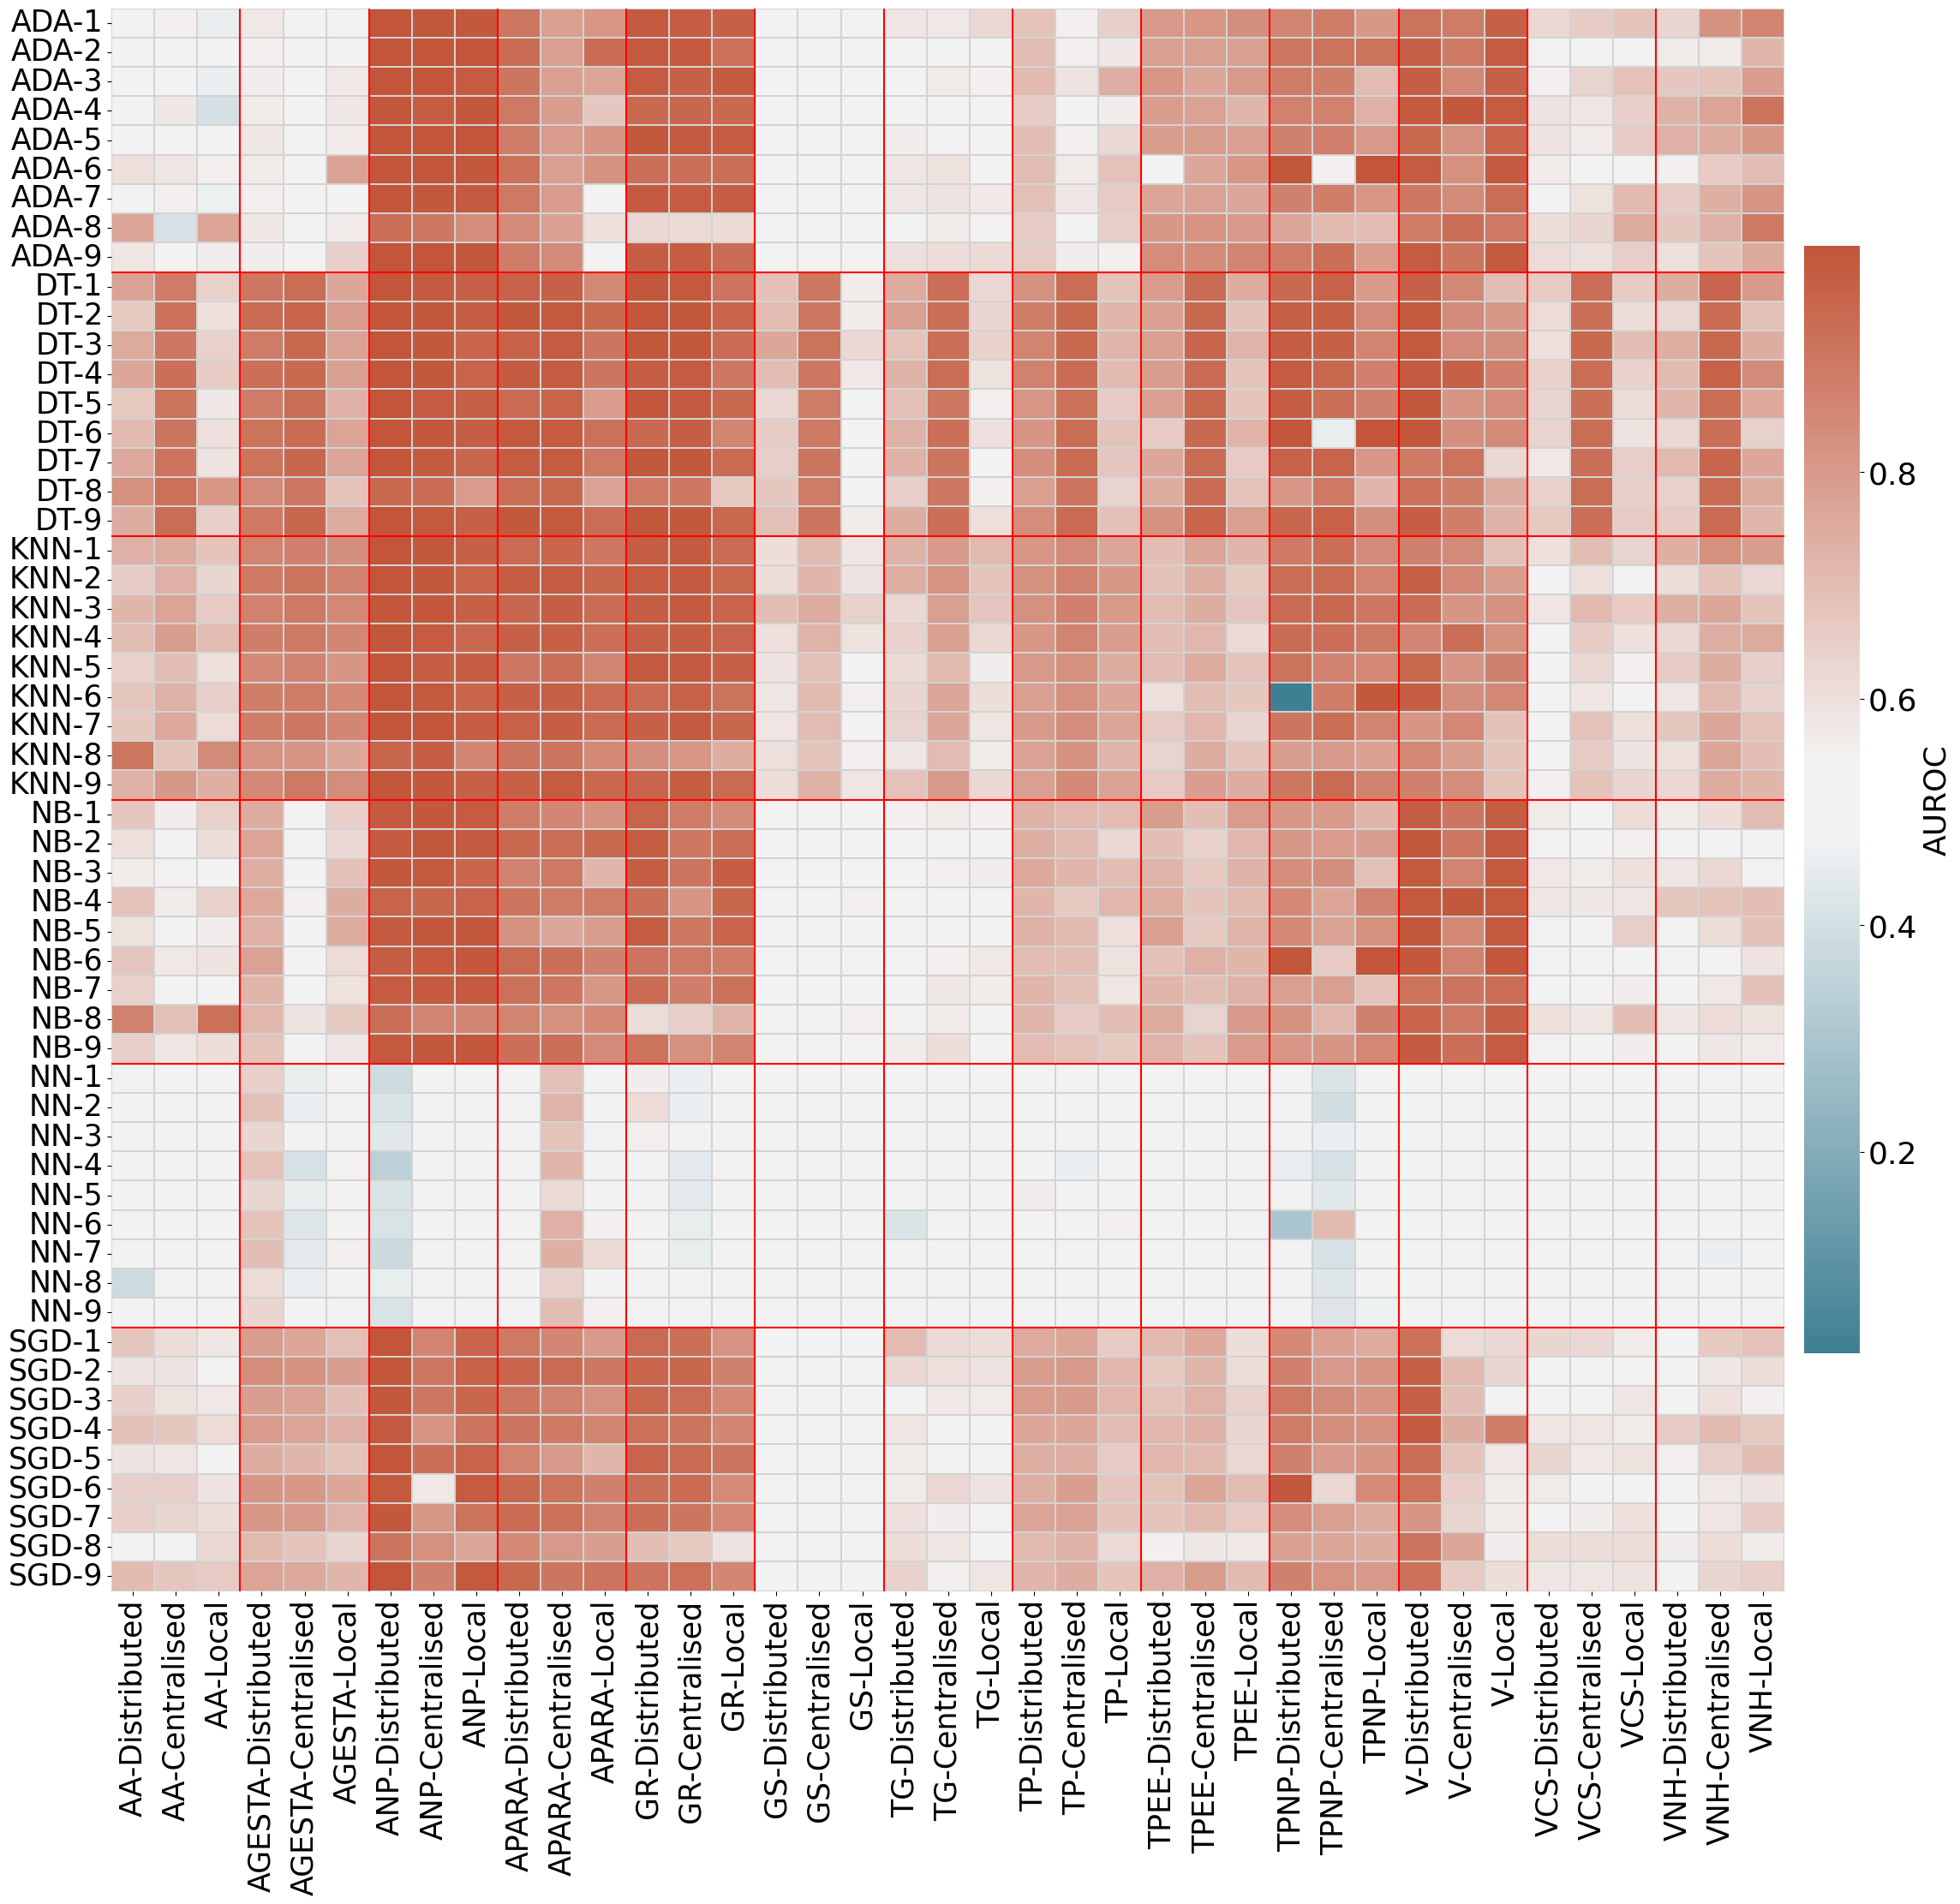
\includegraphics[scale=0.22]{figures/heatmap-class.png}
\end{figure}
%TC:endignore
%TC:ignore

\begin{figure}[htbp]
\centering
\captionsetup{justification=centering}

\caption[Heatmap of regression algorithm and silo vs Target variable and model type.]{Heatmap of regression algorithm and silo vs Target variable and model type. Value is the MAE mean of all 10 experiments. The y axis is the algorithm and silo. X axis is Target variable and Method. IA - Mother Age; IGA - Weeks on Admission; IMC - BMI; NRCPN - Nr of consultations; PI - Weight start of pregnancy; SGP - Weeks on Delivery;}\label{fig:heatmpa-int} 
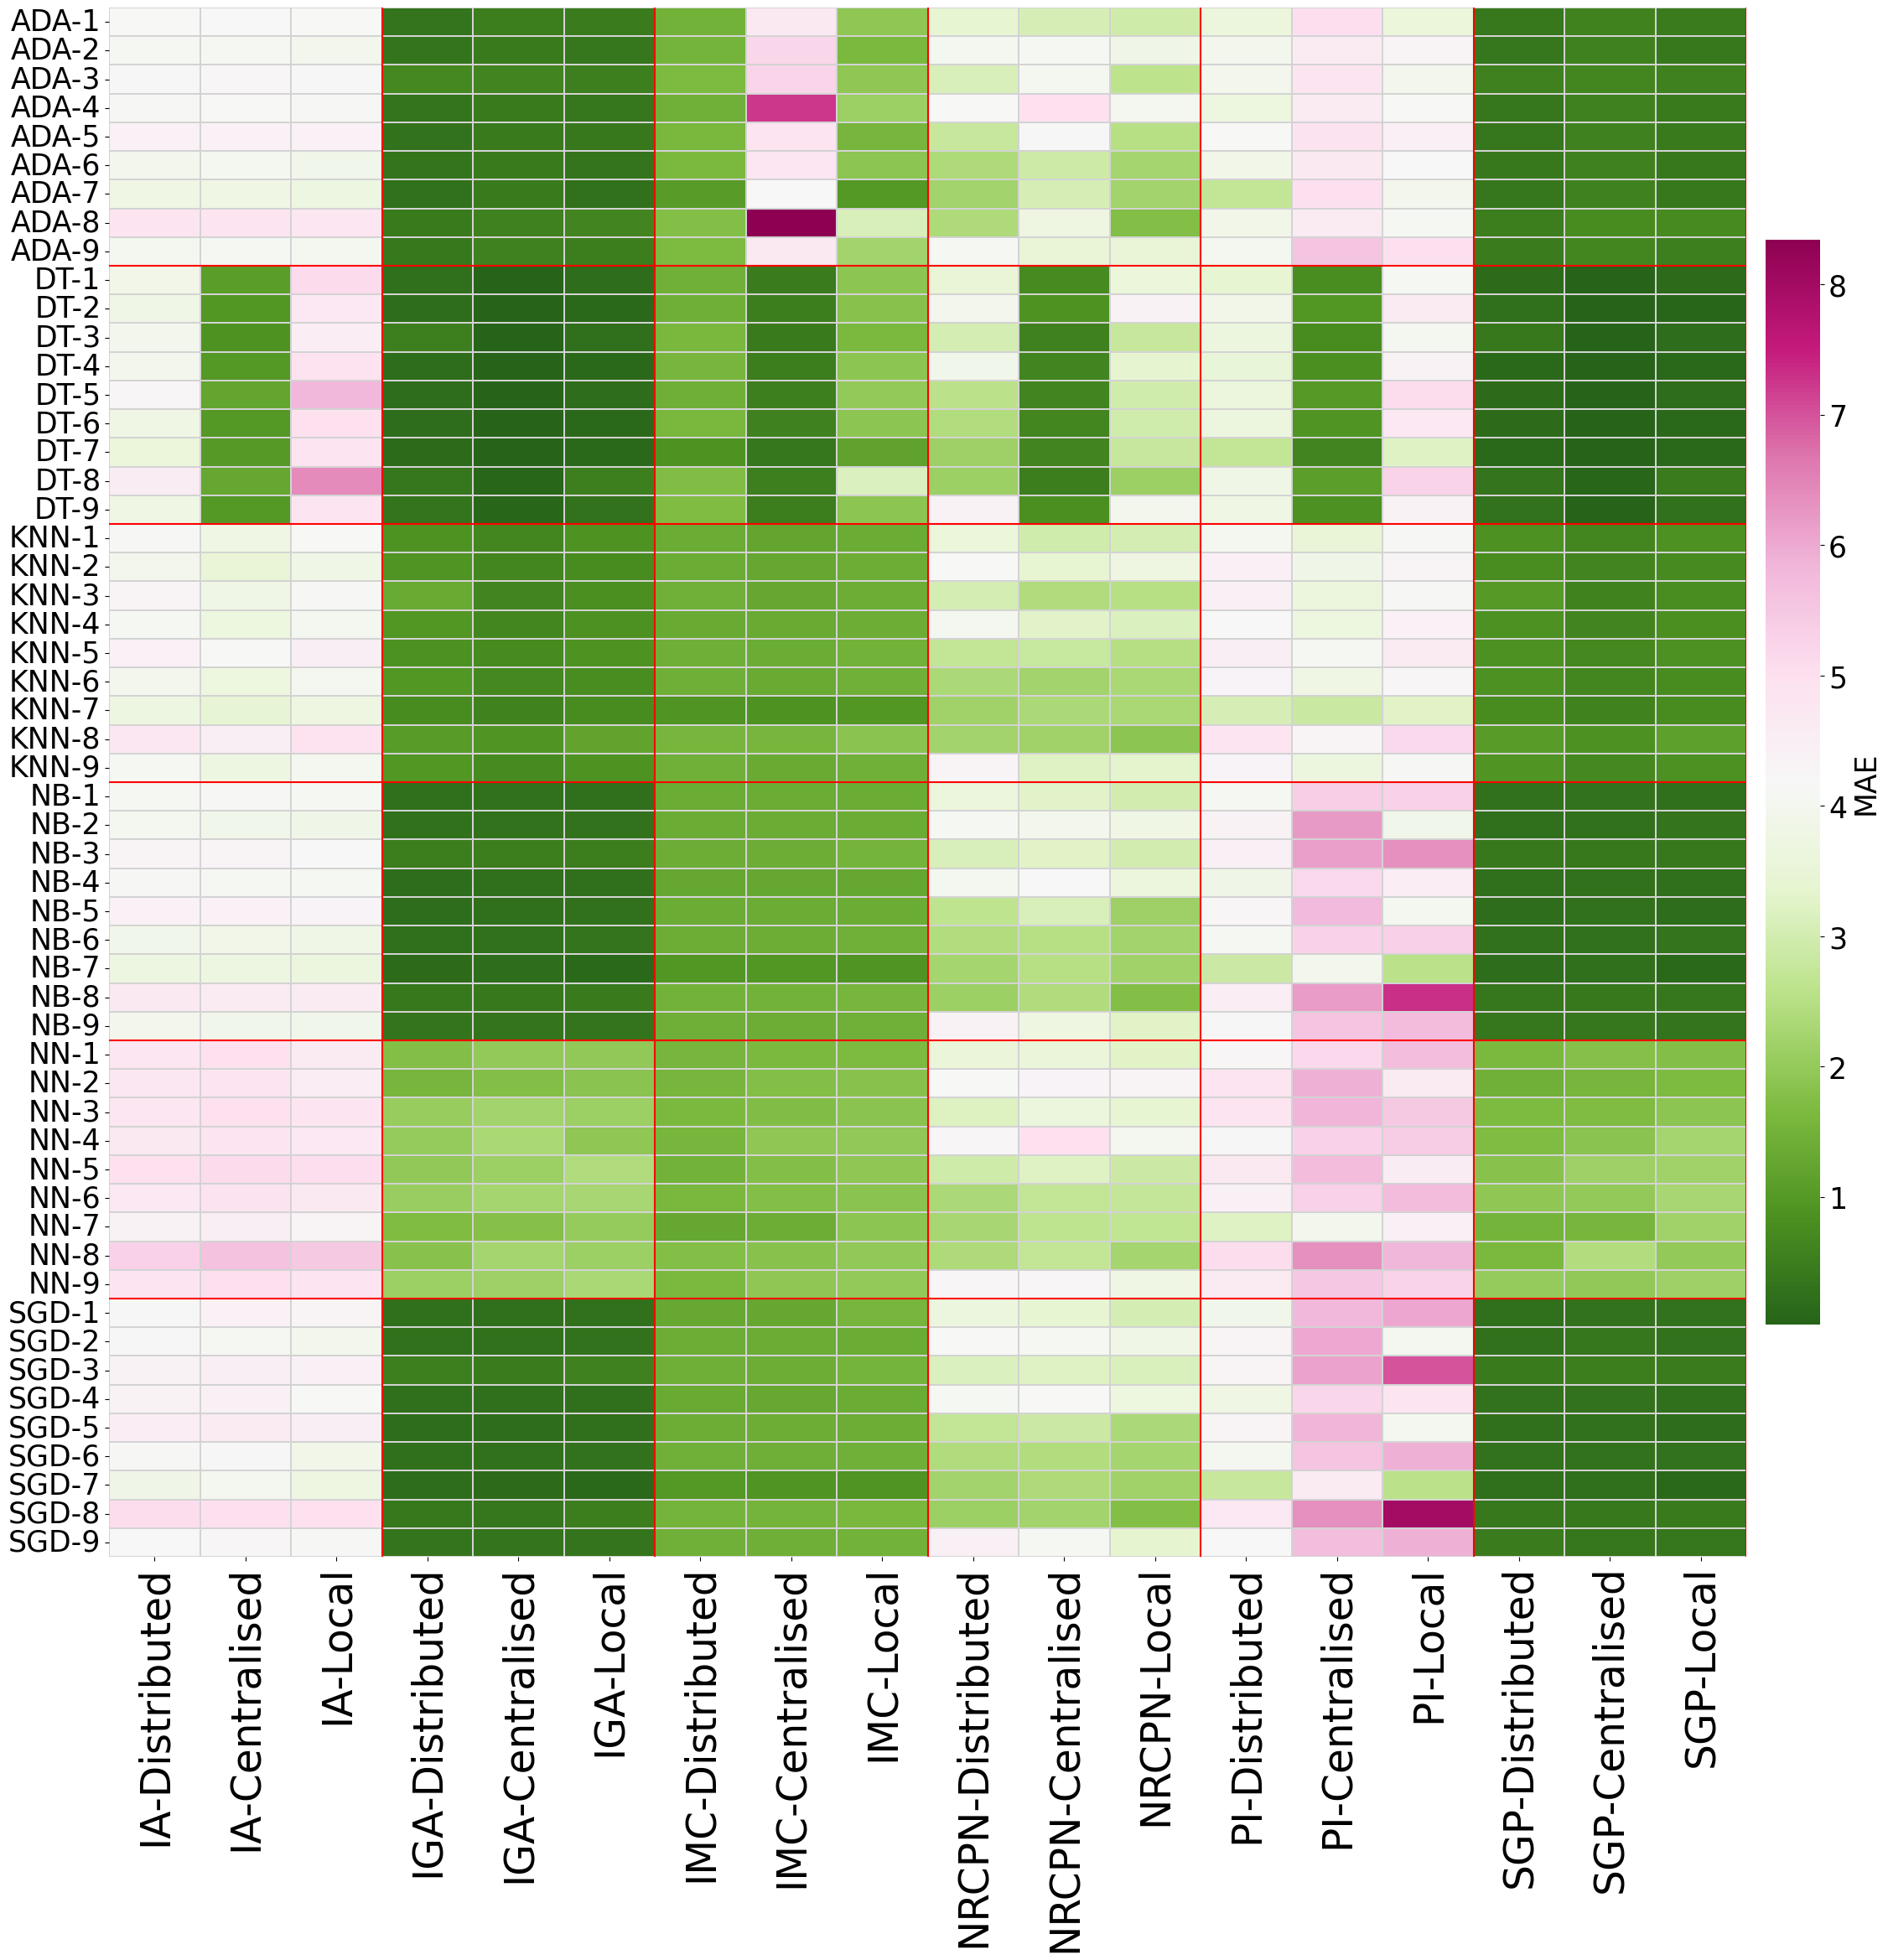
\includegraphics[scale=0.22]{figures/heatmap-reg.png}
\end{figure}
%TC:endignore

{\small
\definecolor{Gray}{gray}{0.85} 
 \begin{table}[h] 
 \setlength{\tabcolsep}{6pt} % Default value: 6pt 
 \renewcommand{\arraystretch}{1.1} % Default value: 1
  \captionsetup{justification=centering} 
\centering
\caption[Model comparison: Distributed versus centralised and local for every test]{Model comparison: Distributed versus centralised and local for every test. Each cell is the total of distributed model when compared with centralised model (row) and local model (column) across different silos and outcome variable. ($>$ for better, = for non significance and $<$ for worse). The first example is 72 which means that 72 iterations of the distributed SGD was better than the centralised and local. SGD: Stochastic Gradient Descent, NN: Neural Network, KNN: K-Nearest Neighbors, ADA: AdaBoost, NB: Naive Bayes, DT: Decision Tree. Comparison was done with 2-sample T-test with a $\alpha$ of 0.05. (\% in parentheses)}
\label{tab:hyp}
\begin{tabular}{llrrrr}
\toprule


 &  & Distributed $>$ Local & Distributed = Local & Distributed $<$ Local & \textbf{Row Total} \\


\hline \multirow{3}{*}{SGD} &Distributed $>$ Centralised  & 72 (7.0) & 14 (1.4) & 9 (0.8) & \textbf{95 (9.3)} \\
 & Distributed =  Centralised& 14 (1.4) & 17 (1.7) & 6 (0.6) & \textbf{37 (3.6) } \\
 & Distributed $<$ Centralised  & 11 (1.1) & 11 (1.1) & 17 (1.7) & \textbf{39 (3.8)} \\
% \hline
% \multicolumn{2}{c|}{SGD Total} & 97 (9.4)&42 (4.1) &32 (18.7)& \textbf{171}  \\
\hline \multirow{3}{*}{NN} & Distributed $>$ Centralised & 44 (4.3) & 44 (4.3) & 7 (0.7) & \textbf{95 (9.3)} \\
 & Distributed =  Centralised& 2 (0.2) & 33 (3.2) & 2 (0.2) & \textbf{37 (3.6)} \\
 & Distributed $<$ Centralised & 0 (0) & 17 (1.7) & 22 (2.1) & \textbf{39 (3.8)} \\
% \hline

% \multicolumn{2}{c|}{NN Total} & 46&94 &31 & \textbf{171}  \\

\hline \multirow{3}{*}{KNN} & Distributed $>$ Centralised & 16 (1.6) & 0 (0) & 1 (0.1) & \textbf{17 (1.7)} \\
 & Distributed =  Centralised & 10 (1) & 2 (0.2) & 1 (0.1) & \textbf{13 (1.3)} \\
 & Distributed $<$ Centralised & 72 (7)  & 28 (2.7) & 41 (4) & \textbf{141 (13.7)} \\
% \hline

% \multicolumn{2}{c|}{KNN Total} & 97&30 &43 & \textbf{171}  \\

\hline \multirow{3}{*}{ADA} & Distributed $>$ Centralised & 64 (6.2) & 25 (2.4) & 22 (2.1) & \textbf{111 (10.8)} \\
 & Distributed =  Centralised& 5 (0.5) & 12 (1.2) & 10 (1) & \textbf{27(2.6)} \\
 & Distributed $<$ Centralised & 10 (1) & 6 (0.6) & 17 (1.7) & \textbf{33 (3.2)} \\
% \hline

% \multicolumn{2}{c|}{ADA Total} & 79&43 &49 & \textbf{171}  \\

\hline \multirow{3}{*}{NB} & Distributed $>$ Centralised & 51 (5) & 19 (1.9) & 34 (3.3) & \textbf{104 (10.1) } \\
 &  Distributed =  Centralised & 5 (0.5) & 19 (1.9) & 12 (1.2) & \textbf{36 (3.5)} \\
 & Distributed $<$ Centralised  & 3 (0.3) & 4 (0.4) & 24 (2.3) & \textbf{31 (3)} \\
% \hline

% \multicolumn{2}{c|}{NB Total} & 59&42 &70 & \textbf{171}  \\

\hline \multirow{3}{*}{ DT} & Distributed $>$ Centralised & 27 (2.6) & 0 (0) & 1 (0.1) & \textbf{28 (2.7)} \\
 & Distributed = Centralised & 8 (0.8) & 0 (0) & 0 (0)& \textbf{8 (0.8)} \\
 & Distributed $<$ Centralised & 97 (9.5) & 12 (1.2) & 26 (2.5) & \textbf{135 (13.2)} \\
% \hline

% \multicolumn{2}{c|}{DT Total} & 132&12 &27 & \textbf{171}  \\
 
 \hline
  \textbf{Total} &  & \textbf{511 (49.8)} & \textbf{263 (25.6)} & \textbf{252 (24.6)} & \textbf{1026 (100)}\\
 \bottomrule
\end{tabular}
\end{table}
}
















\subsection{Discussion}
% !TeX root = ../../thesis.tex



A significant finding is that nearly 59\% of distributed models demonstrated comparable, if not superior, performance relative to their centralised counterparts (table \ref{tab:hyp} last column, first two values for each algorithm). From these, 41.9\% were also better or equal to the local model. If we take the best performing algorithm (SGD), we have 77.2\% for distributed better than centralised and 66\% better than centralised and local. This outcome underlines the potential of distributed models to offer reliable inference capabilities that match those of traditional centralised models, without sacrificing predictive accuracy. Furthermore, the adoption of distributed models enhances privacy for data owners, presenting a compelling case for their broader application in data-sensitive environments. Overall, our results suggest that it is possible to implement a distributed model without significantly losing information. Our analysis suggests that SGD, Adaboost and Naive Bayes approaches are suitable for such distributed approached with tabular data. However, MLPerceptron, Decision Trees and \ac{knn} do not seem to be a good approach for such use cases.

However, there are still issues to be addressed. This methodology presents hurdles regarding categorical class handling. Firstly, all classes should be known first-hand and should be given to each model even if that silo in particular has no cases of that class. Secondly, low-frequency classes are also an issue to be addressed, since training the model with cross-validation will raise problems because each split should have all classes present. Our approach relied on sample creation for low and non-existent target classes. However, this approach is adding information to the model that is not originally there. The way we chose for minimising this issue was by creating dummy variables with median and mode imputations based only on the information in the dataset. Nevertheless, non-existent classes are impossible to address without prior information. These class problems could be partially tackled in production by implementing data management and governance procedures, namely data dictionaries. Still on data preprocessing, we applied ordinal encoding to the variables which will create a natural hierarchy between variables. One solution for this is to create binary columns for each class in each column. This will remove the hierarchy between classes but increase variable numbers and training time considerably.\\

Another issue to consider is the path adopted to build the distributed model. In this case, it was decided to develop an ensemble of models with voting. However, other methods could have been employed, like parameter averaging, that should be tested as well. In particular, the usage of more robust neural networks could be assessed as well. We chose not to test state-of-the-art neural networks since the data volume was low for that use case and several papers have already demonstrated that neural networks are not the most suitable tool for tabular data \cite{grinsztajnWhyTreebasedModels2022,borisovDeepNeuralNetworks2022}. We chose to add MLPerceptron as a baseline for comparison with the remaining algorithms. The results show us that the performance was below the other algorithms, but in this concrete case, the problem may reside in the architecture chosen and hyperparameters used in the Cross-validation which may have lead to underfitting. Despite this, a precise and thorough demonstration of this use case would be important to consider such scenarios. \\
Furthermore, the algorithm underlying the distributed model is of importance as well for its performance versus the centralised model. Figures \ref{fig:heatmap-cat} and \ref{fig:heatmpa-int} and table \ref{tab:hyp} show us that Decision trees and \ac{knn} implemented in a centralised manner are consistently better than the distributed counterpart. This is specially notorious in the case of the decision trees. We believe this may be related to way the algorithm is implemented. A centralised version may be able to create optimal splits in the data, while the distributed version may not be able to do so. This is a topic that should be further explored.\\
Even though this improvement may have a relationship to the target variable (i.e. figure \ref{fig:heatmpa-int} for IA and IGA variables), it is still an important fact to take into account when implementing such architectures.
The performance of the models is also interesting to catch differences in silos. See silo 6 for TPNP (figure \ref{fig:heatmap-cat}) where silo 6 consistently behaves differently than the rest.
Checking performance data regarding regression tasks, we can see a drop in performance for PI and IA. While the explanation for the performance of IA can be explained by the average value of it which is 66. This is the highest average in the dataset. This means that the model will have a harder time predicting these values. This is also true for the distributed model. This is a topic that should be further explored.\\
As for implementation, such a mechanism could be implemented in at least two manners; with a central orchestrator or without. The first one would assume a central point that would make a request to each silo for a prediction and then create the final prediction with the weighted averaging of each one. The second one would not require any additional platform and each silo would communicate with each of the others and receive the prediction and would create the final with their own. This implementation step would of course take into account variables that we were out of scope such as the communication between silos. 
Regarding the prediction capability as a whole, we found that this data is suitable to apply machine-learning models in order to predict several clinical outcomes, with very good results for several target variables. 


\subsection{Conclusion}
Bud1hh` 0x8 OBS  @� @� @� @$imagens-tese.jpgIlocblob���������imagens-tese.pptxIlocblob����������LivrosIlocblob����������Livrosbwspblob�bplist00�	]ShowStatusBar[ShowToolbar[ShowTabView_ContainerShowSidebar\WindowBounds[ShowSidebar			_{{-1920, 0}, {1728, 1055}}	#/;R_klmno�
�LivrosvSrnlongmetadata Sonho.xlsxIlocblobA&������
NewsletterIlocblob�&��������
obs-cdss-fhirIlocblob&������
obs-model.pngIlocblob.������Outras apresentac'oesIlocblob�&��������Outras apresentac'oesbwspblob�bplist00�	]ShowStatusBar[ShowToolbar[ShowTabView_ContainerShowSidebar\WindowBounds[ShowSidebar			_{{-1920, 0}, {1920, 1055}}	#/;R_klmno�
�Outras apresentac'oeslg1ScompOutras apresentac'oesmoDDblob�[�&��AOutras apresentac'oesmodDblob�[�&��AOutras apresentac'oesph1ScompOutras apresentac'oesvSrnlongPapersIlocblob�&��������Papersbwspblob�bplist00�	]ShowStatusBar[ShowToolbar[ShowTabView_ContainerShowSidebar\WindowBounds[ShowSidebar			_{{272, -208}, {1920, 1055}}	#/;R_klmno�
�PapersvSrnlongpesquisas pubmed.xlsxIlocblobg&��������Report teseIlocblob�������Report tesebwspblob�bplist00�	]ShowStatusBar[ShowToolbar[ShowTabView_ContainerShowSidebar\WindowBounds[ShowSidebar			_{{0, 0}, {1920, 1055}}	#/;R_klmno�
�Report teselg1ScompReport tesemoDDblob���+�0�AReport tesemodDblob���+�0�AReport teseph1ScompReport tesevSrnlong
response.docxIlocblob�������response.pdfIlocblob��������	reunioesIlocblob��������	reunioesbwspblob�bplist00�	]ShowStatusBar[ShowToolbar[ShowTabView_ContainerShowSidebar\WindowBounds[ShowSidebar			_{{-1636, 161}, {1186, 604}}	#/;R_klmno�
�	reunioesvSrnlongreviewsIlocblob��������reviewsbwspblob�bplist00�	]ShowStatusBar[ShowToolbar[ShowTabView_ContainerShowSidebar\WindowBounds[ShowSidebar			_{{-1920, 0}, {1920, 1055}}	#/;R_klmno�
�reviewsvSrnlongtitle-page.docxIlocblob��������0. thesis-supportIlocblobA.��������1. repositorio de dadosIlocblob�.������2. dados sinteticosIlocblob.������2. dados sinteticosbwspblob�bplist00�	]ShowStatusBar[ShowToolbar[ShowTabView_ContainerShowSidebar\WindowBounds[ShowSidebar			_{{2228, 501}, {920, 436}}	#/;R_klmno�
�2. dados sinteticosvSrnlong2.1 pedidos instituic'oesIlocblob�.��������2.1 pedidos instituic'oesbwspblob�bplist00�	]ShowStatusBar[ShowToolbar[ShowTabView_ContainerShowSidebar\WindowBounds[ShowSidebar			_{{452, 125}, {1220, 709}}	#/;R_klmno�
�2.1 pedidos instituic'oesvSrnlong3.1 survey GANIlocblob�.������3.1 survey GANbwspblob�bplist00�	]ShowStatusBar[ShowToolbar[ShowTabView_ContainerShowSidebar\WindowBounds[ShowSidebar			_{{179, 121}, {1186, 604}}	#/;R_klmno�
�3.1 survey GANvSrnlong3.2 phd consortium aimeIlocblobg.������3.4 survey fullIlocblobA�������3.6 distributed learningIlocblob����������3.6 distributed learningbwspblob�bplist00�]ShowStatusBar[ShowToolbar[ShowTabView_ContainerShowSidebar\WindowBounds[ShowSidebar				_{{0, 0}, {1728, 1055}}	#/;R_klmno�
�3.6 distributed learningicvpblob�bplist00�	

_backgroundColorBlueXiconSizeXtextSize_backgroundColorRed^backgroundType_backgroundColorGreen[gridOffsetX_scrollPositionY[gridOffsetY\showItemInfo_viewOptionsVersion_scrollPositionXYarrangeBy]labelOnBottom_showIconPreview[gridSpacing#?�#@P#@(#Tnone		#@K+AJShw��������"+4=?HIZ_`aj3.6 distributed learningvSrnlong3.7 analise dadosIlocblob�������3.7 analise dadosbwspblob�bplist00�	]ShowStatusBar[ShowToolbar[ShowTabView_ContainerShowSidebar\WindowBounds[ShowSidebar			_{{179, 121}, {1186, 604}}	#/;R_klmno�
�3.7 analise dadosvSrnlong
3.8 OBS MLIlocblob����������
3.8 OBS MLbwspblob�bplist00�	]ShowStatusBar[ShowToolbar[ShowTabView_ContainerShowSidebar\WindowBounds[ShowSidebar			_{{0, 0}, {1728, 1055}}	#/;R_klmno�
�
3.8 OBS MLicvpblob�bplist00�	

_backgroundColorBlue_showIconPreviewXtextSize_backgroundColorRed^backgroundType_backgroundColorGreen[gridOffsetX_scrollPositionY[gridOffsetY\showItemInfo_viewOptionsVersion_scrollPositionXYarrangeBy]labelOnBottomXiconSize[gridSpacing#?�	#@(#\dateModified	#@P#@K+AS\q���������
"+,57@AR_`ir
3.8 OBS MLlsvpblob�bplist00�	

HIJKMXiconSize_showIconPreviewWcolumns_calculateAllSizes_scrollPositionYXtextSize_scrollPositionXZsortColumn_useRelativeDates_viewOptionsVersion#@0	� %*/48=BXcommentsUlabelWversion[dateCreatedTsize\dateModifiedTkindTname^dateLastOpened�UindexUwidthYascendingWvisible,	�!"d	�&'K	�+,��01a	�5,	�9:s		�>?:		�CD�#@3#@*#Tname	&8@Tfo������������(.4>FHKLMVXZ[\egijktvxyz������������������������������N�
3.8 OBS MLvSrnlong3.9 Catalogar DatasetIlocblob����������3.9 Catalogar Datasetbwspblob�bplist00�	]ShowStatusBar[ShowToolbar[ShowTabView_ContainerShowSidebar\WindowBounds[ShowSidebar			_{{-1516, 283}, {1206, 635}}	#/;R_klmno�
�3.9 Catalogar Dataseticvpblob�bplist00�	

_backgroundColorBlue_showIconPreviewXtextSize_backgroundColorRed^backgroundType_backgroundColorGreen[gridOffsetX_scrollPositionY[gridOffsetY\showItemInfo_viewOptionsVersion_scrollPositionXYarrangeBy]labelOnBottomXiconSize[gridSpacing#?�	#@(#Tnone	#@P#@K+AS\q���������
"+,57@ARWXaj3.9 Catalogar Datasetlg1Scomp3.9 Catalogar DatasetmoDDblobZ$8����A3.9 Catalogar DatasetmodDblobZ$8����A3.9 Catalogar Datasetph1Scomp3.9 Catalogar DatasetvSrnlong4.0 IPOPIlocblobg�������4.0 IPOPbwspblob�bplist00�	]ShowStatusBar[ShowToolbar[ShowTabView_ContainerShowSidebar\WindowBounds[ShowSidebar			_{{0, 0}, {1920, 1055}}	#/;R_klmno�
�4.0 IPOPicvpblob�bplist00�	

_backgroundColorBlue_showIconPreviewXtextSize_backgroundColorRed^backgroundType_backgroundColorGreen[gridOffsetX_scrollPositionY[gridOffsetY\showItemInfo_viewOptionsVersion_scrollPositionX]labelOnBottomYarrangeByXiconSize[gridSpacing#?�	#@(#	Tnone#@P#@K+AS\q��������
"+,57@ARSXaj4.0 IPOPvSrnlong5.0 historia SISIlocblobA*��������6.0 logs HospitaisIlocblob�*������6.0 logs Hospitaisbwspblob�bplist00�	]ShowStatusBar[ShowToolbar[ShowTabView_ContainerShowSidebar\WindowBounds[ShowSidebar			_{{-1920, 0}, {1920, 1055}}	#/;R_klmno�
�6.0 logs Hospitaisicvpblob�bplist00�	

_backgroundColorBlue[gridSpacingXtextSize_backgroundColorRed^backgroundType_backgroundColorGreen[gridOffsetX_scrollPositionY[gridOffsetY\showItemInfo_viewOptionsVersion_scrollPositionXYarrangeBy]labelOnBottomXiconSize_showIconPreview#?�#@K#@(#Tnone	#@P	+AMVkz��������"+4=?HIZ_`ij6.0 logs HospitaisvSrnlong7.0 Data qualityIlocblob*��������7.0 Data qualitybwspblob�bplist00�	]ShowStatusBar[ShowToolbar[ShowTabView_ContainerShowSidebar\WindowBounds[ShowSidebar			_{{0, 0}, {1728, 1055}}	#/;R_klmno�
�7.0 Data qualitylsvCblob5bplist00�	

TUVWX_viewOptionsVersion_showIconPreviewWcolumns_calculateAllSizes_scrollPositionYXtextSize_scrollPositionXZsortColumnXiconSize_useRelativeDates	�!%*/49=BFJN�WvisibleUwidthYascendingZidentifier	,	Tname�Xubiquity#� 	�\dateModified�$[dateCreated�')	aTsize�,.	s	Tkind�13d	Ulabel�68K	Wversion�<	Xcomments�?A�^dateLastOpened�?EZshareOwner�?I_shareLastEditor�KYdateAdded�PR�_invitationStatus#@G�#@*#Tname#@0	2DL`r{����������� !*+-.;DEFR[\^_dmnpqv�������������������������
 "#67@IRW`Za7.0 Data qualitylsvpblob�bplist00�	

GHIJK_viewOptionsVersion_showIconPreviewWcolumns_calculateAllSizes_scrollPositionYXtextSize_scrollPositionXZsortColumnXiconSize_useRelativeDates	� %*/48=AXcommentsUlabelWversion[dateCreatedTsize\dateModifiedTkindTname^dateLastOpened�UindexUwidthYascendingWvisible,	�!"d	�&'K	�+,��01a	�5,	�9:s		�>		�BC�#@G�#@*#Tname#@0	2DL`r{�����������'06<FNPSTU^`bcdmoqrs|~��������������������������������M�7.0 Data qualityvSrnlong8.0 dataset similarityIlocblob�*��������8.0 dataset similaritybwspblob�bplist00�	]ShowStatusBar[ShowToolbar[ShowTabView_ContainerShowSidebar\WindowBounds[ShowSidebar			_{{-1654, 142}, {1091, 843}}	#/;R_klmno�
�8.0 dataset similaritylsvCblob*bplist00�	

TUTVXXiconSize_showIconPreviewWcolumns_calculateAllSizes_scrollPositionYXtextSize_scrollPositionXZsortColumn_useRelativeDates_viewOptionsVersion#@0	�!%*/49=BFJN�ZidentifierYascendingUwidthWvisibleTname	,	�Xubiquity#�\dateModified�	�"[dateCreated�&(Tsizea	�+-Tkind	s	�02Ulabel	d�57Wversion	K�:Xcomments	�>@^dateLastOpened��C@ZshareOwner�G@_shareLastEditor�KYdateAdded�PR�_invitationStatus##@*Tname	&8@Tfo��������������"/023<HIJSXY[\ejkmnw}~������������������������
./8AFGYX8.0 dataset similaritylsvpblob�bplist00�	

GHGIKXiconSize_showIconPreviewWcolumns_calculateAllSizes_scrollPositionYXtextSize_scrollPositionXZsortColumn_useRelativeDates_viewOptionsVersion#@0	� %*/48=AXcommentsUlabelWversion[dateCreatedTsize\dateModifiedTkindTname^dateLastOpened�WvisibleYascendingUwidthUindex	,�#$	d�()	K�-.��23	a�-7	�;<		s�@		�DE�##@*Tname	&8@Tfo������������(0:@FGHKMVWXZ\efgiktuvxz����������������������������L�8.0 dataset similarityvSrnlong9.0 benchmark clusterIlocblob�*������9.0 benchmark clusterbwspblob�bplist00�	]ShowStatusBar[ShowToolbar[ShowTabView_ContainerShowSidebar\WindowBounds[ShowSidebar			_{{211, 219}, {1186, 604}}	#/;R_klmno�
�9.0 benchmark clustervSrnlong99. Process MiningIlocblobg*������99. Process MiningvSrnlong-Captura de ecra 2023-12-06, as 16.25.16.pngIlocblob�.������-Captura de ecra 2023-12-06, as 16.25.26.pngIlocblobC.������-Captura de ecra 2024-02-26, as 10.44.33.pngIlocblob�.������1Captura de ecra 2024-03-26, as 14.13.56 (2).pngIlocblob�.������-Captura de ecra 2024-03-26, as 14.14.05.pngIlocblobi.������-Captura de ecra 2024-03-26, as 14.16.27.pngIlocblob��������clinical_assessment.pngIlocblob�.������dec-tese-rjc.pdfIlocblobC�������DocsIlocblobA���������Docsbwspblob�bplist00�	]ShowStatusBar[ShowToolbar[ShowTabView_ContainerShowSidebar\WindowBounds[ShowSidebar			_{{0, 0}, {1920, 1055}}	#/;R_klmno�
�DocsvSrnlongExemplos outras pessoasIlocblob��������Exemplos outras pessoasbwspblob�bplist00�	]ShowStatusBar[ShowToolbar[ShowTabView_ContainerShowSidebar\WindowBounds[ShowSidebar			_{{490, 144}, {1091, 843}}	#/;R_klmno�
�Exemplos outras pessoaslg1ScompExemplos outras pessoasmoDDblob��b3�AExemplos outras pessoasmodDblob��b3�AExemplos outras pessoasph1ScompExemplos outras pessoasvSrnlongFinalIlocblobC������heads-thesisIlocblob��������heads-thesisbwspblob�bplist00�	]ShowStatusBar[ShowToolbar[ShowTabView_ContainerShowSidebar\WindowBounds[ShowSidebar			_{{2420, 422}, {920, 492}}	#/;R_klmno�
�heads-thesislsvCblob:bplist00�	

UVWXZXiconSize_showIconPreviewWcolumns_calculateAllSizes_scrollPositionYXtextSize_scrollPositionXZsortColumn_useRelativeDates_viewOptionsVersion#@0	�!%*/49>CGKO�ZidentifierUwidthYascendingWvisibleTname0		�Xubiquity#�\dateModified�	�"[dateCreated�&'Tsizea	�+,Tkinds		�01Ulabeld	�56WversionK	�:;Xcomments,	�?@^dateLastOpened��D@ZshareOwner�H@_shareLastEditor�LYdateAdded�QS�_invitationStatus#@a`#@*#Tname	&8@Tfo�������������"/123<HIJSXZ[\ejlmnw}�������������������������12;DMRS[dheads-thesislsvpblob�bplist00�	

HIJKMXiconSize_showIconPreviewWcolumns_calculateAllSizes_scrollPositionYXtextSize_scrollPositionXZsortColumn_useRelativeDates_viewOptionsVersion#@0	� %*/48=BXcommentsUlabelWversion[dateCreatedTsize\dateModifiedTkindTname^dateLastOpened�WvisibleUwidthYascendingUindex,	�"$d	�')K	�,.��13	a�,7	�:<	s	�?A	0	�DF�#@a`#@*#Tname	&8@Tfo������������(06@FGJKMVWYZ\efhiktuwxz������������������������������N�	]ShowStatusBar[ShowToolbar[ShowTabView_ContainerShowSidebar\WindowBounds[ShowSidebar			_{{211, 219}, {1186, 604}}	#/;R_klmno�
�9.0 benchmark clustervSrnlong99. Process MiningIlocblobg*������
3.8 OBS MLlsvCblob:bplist00�	

UVWXZXiconSize_showIconPreviewWcolumns_calculateAllSizes_scrollPositionYXtextSize_scrollPositionXZsortColumn_useRelativeDates_viewOptionsVersion#@0	�!%*/49>CGKO�WvisibleUwidthYascendingZidentifier	:	Tname�#Xubiquity� 	�\dateModified�$[dateCreated�')	aTsize�,.	s	Tkind�13d	Ulabel�68K	Wversion�;=,	Xcomments�@B�^dateLastOpened�@FZshareOwner�@J_shareLastEditor�NYdateAdded�PQ_invitationStatus�#@3#@*#Tname	&8@Tfo���������������
"#%&3<=>JSTVW\efhinwxz{������������������������-/012;DMRS[d7.0 Data qualityicvpblob�bplist00�	

_backgroundColorBlue[gridSpacingXtextSize_backgroundColorRed^backgroundType_backgroundColorGreen[gridOffsetX_scrollPositionY[gridOffsetY\showItemInfo_viewOptionsVersion_scrollPositionXYarrangeBy]labelOnBottom_showIconPreviewXiconSize#?�#@K#@(#Tnone		#@P+AMVkz��������"+4=?HIZ_`aj99. Process Miningbwspblob�bplist00�	]ShowStatusBar[ShowToolbar[ShowTabView_ContainerShowSidebar\WindowBounds[ShowSidebar			_{{138, 192}, {920, 492}}	#/;R_klmno�
�heads-thesisvSrnlongb��b3�AExemplos outras pessoasmodDblob��b3�AExemplos outras pessoasph1ScompExemplos outras pessoasvSrnlongFinalIlocblobC������heads-thesisIlocblob��������heads-thesisbwspblob�bplist00�	]ShowStatusBar[ShohE` 0@PDSDB `�p� @� @Tnone		#@P+AMVkz��������"+4=?HIZ_`aj99. Process Miningbwspblob�bplist00�	]ShowStatusBar[ShowToolbar[ShowTabView_ContainerShowSidebar\WindowBounds[ShowSidebar			_{{138, 192}, {920, 492}}	#/;R_klmno�
�heads-thesisvSrnlongb��b3�AExemplos outras pessoasmodDblob��b3�AExemplos outras pessoasph1ScompExemplos outras pessoasvSrnlongFinalIlocblobC������heads-thesisIlocblob��������heads-thesisbwspblob�bplist00�	]ShowStatusBar[Sho


\section{Can Institutions share their performance metrics without hesitation of retaliation?}\label{subsec:benchmark}
This section is based on the paper entitled "Benchmarking institutions' health outcomes with clustering methods". This paper was focused on the fact that many healthcare institutions harbor reservations about openly sharing production metrics. One predominant concern is the potential for retaliatory actions, be it from regulatory bodies, competitors, or the public. In this paper, we propose the application of a clustering methodology that allows institutions to compare performance metrics without disclosing the actual values. The method is based on clustering, which involves grouping health institutions' outcomes into a known number of clusters, allowing institutions to position themselves in a range of clusters without sharing the true means of their target data. The proposed method uses the K-means and K-modes clustering algorithms and was tested on data from real Electronic health records and public datasets. This approach provides a valid benchmark of hospital metrics and performances while protecting the privacy of participating institutions. 
\subsection{Introduction}
Health institutions play a critical role in providing essential healthcare services to communities and ensuring that they operate efficiently and effectively is crucial. Benchmarking is a process that allows hospitals to compare their performance against that of other institutions, which can help identify areas of strength and weakness \cite{suydamPatientSafetyData2007}. By analyzing and evaluating performance metrics, such as patient outcomes, operational efficiency, and financial management, hospitals can identify best practices and make data-driven decisions to improve their overall performance. It can also help hospitals identify and implement innovative practices that can lead to better patient care and improved staff satisfaction \cite{hulsenSharingCaringData2020}.

However, despite the numerous benefits of benchmarking, some hospitals may be hesitant to participate due to concerns about revealing weaknesses or being perceived as inferior to their peers. The fear of being judged or penalized for poor performance can sometimes lead hospitals to avoid sharing data, making it difficult to accurately assess their performance and identify areas for improvement. Privacy issues and concerns turn this opportunity into an even less desirable path \cite{hulsenSharingCaringData2020}. To address these concerns, benchmarking initiatives often ensure the confidentiality and anonymity of data to encourage participation and foster trust among participating institutions. However, this is usually not enough. In 2019, as stated in the work of Villanueva et al., \cite{villanuevaCharacterizingBiomedicalDataSharing2019}, 26\% of data-sharing initiatives are based on the aggregation of data and 24\% are based on sharing data in closed consortia. Only 15\% were based on open or controlled access.

To address concerns around privacy and confidentiality, we propose a new method of benchmarking based on clustering. This method involves grouping health institutions' outcomes into a known number of clusters, providing health institutions with the capability of positioning themselves in a range of clusters, without ever sharing the true means of their target data.

This approach to benchmarking not only addresses concerns around privacy and confidentiality. It has the potential to encourage greater participation in benchmarking initiatives, as hospitals can be assured of the anonymity and confidentiality of their data. By creating a more secure and private environment for benchmarking, hospitals can feel more comfortable sharing their data and participating in initiatives that can ultimately improve patient care and operational efficiency.

In conclusion, benchmarking is a crucial tool for hospitals to improve their performance and provide better care for their patients. While concerns around privacy and confidentiality may exist, the clustering approach to benchmarking provides a more accurate assessment of hospital performance while protecting the privacy of participating institutions. By embracing benchmarking initiatives and leveraging new approaches to benchmarking, hospitals can continuously improve their operations and ensure they provide the highest quality of care possible.
In this paper we propose:
\begin{myitemize}
    \item study how to implement clustering mechanism for benchmark
    \item address preprocessing issues for the raw data
    \item highlight pain points to deployment in the real world.
\end{myitemize}
\subsection{Rationale and Related Work}
This work was initially suggested as a follow-up to a previous work of Rodrigues et al., \cite{rodriguesLocalAlgorithmApproximate2018a} where clustering is applied to streaming data sources. We then thought if a similar approach could be applied to healthcare in order to be able to compare data distributions without ever knowing their real values of them.
Clustering in healthcare is often used to create clusters of patients, taking into account a given set of characteristics. This is used to find possible groups of phenotype and be able to characterise populations given the centroids \cite{walkerUnsupervisedLearningTechniques2019,basileInformaticsMachineLearning2018}. It is also used as a method of detecting regularities and patterns in multi-omics data that reveal different molecular subtypes \cite{nicoraIntegratedMultiOmicsAnalyses2020,rappoportMultiomicMultiviewClustering2018}. It can also be used to create unsupervised models for facilitating the annotation of data for supervised models \cite{mcalpineUtilityUnsupervisedMachine2022}. 

K-means \cite{lloydLeastSquaresQuantization1982,steinley2007initializing,macqueen1967classification} is an unsupervised clustering algorithm used to group data points into K distinct clusters based on their similarity. It is widely used in machine learning, data mining, and image segmentation. The algorithm works by randomly initializing K centroids (or cluster centres) and assigning each data point to the nearest centroid. Then, the centroids are moved to the mean of the points assigned to each cluster. This process is repeated until convergence, where the clusters no longer change.

The objective of K-means is to minimize the sum of squared distances between each data point and its assigned centroid, which is also called the within-cluster sum of squares (WCSS). The algorithm attempts to find the best K clusters that minimize the WCSS. However, choosing the right value of K can be challenging, and the algorithm may converge to a suboptimal solution. Therefore, K-means is often run multiple times with different initializations to find the best clustering solution. Despite its simplicity, K-means can be computationally expensive when dealing with large datasets, and it may not work well with non-linearly separable data or when the clusters have different shapes and sizes.

K-modes is another clustering algorithm similar to K-means, but it is designed to work with categorical data. Unlike K-means, which computes the mean of continuous variables, K-modes computes the mode (or the most frequent value) of categorical variables within each cluster. The algorithm works by randomly initializing K centroids and assigning each data point to the nearest centroid based on the number of matching categories. Then, the centroids are moved to the mode of the categories within each cluster. This process is repeated until convergence, where the clusters no longer change.

The objective of K-modes is to minimize the dissimilarity between the data points within each cluster, which is often measured by the Hamming distance, Jaccard distance, or other similarity measures. Like K-means, choosing the right value of K is critical, and the algorithm may converge to a suboptimal solution. Therefore, K-modes is often run multiple times with different initializations to find the best clustering solution. K-modes is particularly useful when dealing with data that have a large number of categorical variables or when the data contain missing values. However, like K-means, K-modes may not work well with non-linearly separable data or when the clusters have different shapes and sizes.

However, as far as we know, this is the first time clustering is tested for exchanging information privately.

\subsection{Materials \& Methods}
\subsubsection{Method Overview}
We used Python 3.9 to implement the mock example of such an use-case. The clustering was done with scikit-learn library \cite{scikit-learn}. The algorithm proposed is shown in algorithm \ref{alg:bench1}.

%TC:ignore
\begin{algorithm}[hbtp]
\caption{Benchmarking with clustering}
\label{alg:bench1}

\SetAlgoLined



\For {variable in silo}{ 
initialize centroids\;
%\begin{itemize}
%    \item real cluster obfuscated with noise
%    \item true centroids
%    \item add noise to data and then create centroids
%\end{itemize}
}
%\SetKwRepeat{Do}{do}{while}
\While{No convergence}{
\begin{itemize}
    \item Send centroids to other silos
\item Receive other silo's information and add own centroids
\item Calculate new centroids
\item calculate score
\end{itemize}
}



\end{algorithm}
%TC:endignore

The method for assessing convergence is based on clustering metrics: the \ac{ri}. This metric computes a similarity measure between two clusters by considering all pairs of samples and counting pairs that are assigned in the same or different clusters in the predicted and true clusters \cite{hubertComparingPartitions1985}. The raw RI score is: $RI = (number\; of\; agreeing\; pairs) / (number\; of\; pairs)$.
Furthermore, convergence must be obtained through several iterations to make sure it's stable, so a buffer period is also important. For the results section, we set the threshold as 0.9 and repetitions at 20.

In this paper, we propose to show how such an implementation could be done while addressing issues with data formats, types and preprocessing. So, we want to check if the encoding of categorical data affects the model and which method is better for encoding such variables. Additionally, we will try to understand if it is possible to create mechanisms for mixed data if categorical and continuous data must be used and evaluated separately and if so, through which mechanisms.
We will test (1) continuous variables alone, and (2) encoded categorical variables as ordinal. We will also test (3) K-modes  and (4) K-means with the proportion of each category for categorical data.
K-means was used as implemented in scikit-learn \cite{scikit-learn} and K-modes, as implemented by J. de Vos \cite{devos2015}.

\subsubsection{Data used}
We used two types of data in this paper. One is simpler and available online from the \ac{uci} dataset library, namely, the heart disease dataset \cite{misc_heart_disease_45}. We made fairly simple preprocessing on that dataset, namely removing the "?" by filling with null and then imputing missing values by imputing the mean on continuous variables and mode on categorical ones. We then separated the data into 3 distinct silos at random to mimic different health institutions.

In order to use real data and address problems found in the wild, we used clinical data gathered from nine different Portuguese hospitals regarding obstetric information, pertaining to admissions from 2019 to 2020. This originated from nine different files representing different sets of patients but with the same features associated with them. The software for collecting data was the same in every institution (although different versions existed across hospitals) - ObsCare. The data columns are the same in every hospital's database. Each hospital was considered a silo for comparison.
\subsection{Results}
As for results, the data from heart disease rendered the figure \ref{fig:cluster_free_3s}. In this, we focused on continuous variables only. For easier reading, the data is as shown in the table \ref{tab:datapoints}. We used data from the real world to test if everything would work similarly, rendering the image \ref{fig:cluster_mydata_9s}. We added a binary category to show how meaningless the value turn in order to get any information out of it.




%TC:ignore

\begin{figure}[htpb]
\centering
\captionsetup{justification=centering}
\caption[Clustering for 3 continuous variables with 3 silos]{Clustering for 3 continuous variables with 3 silos and true centroids (S2) and true means (S2) for example purposes; The values were normalized for visualization purposes with MinMax}
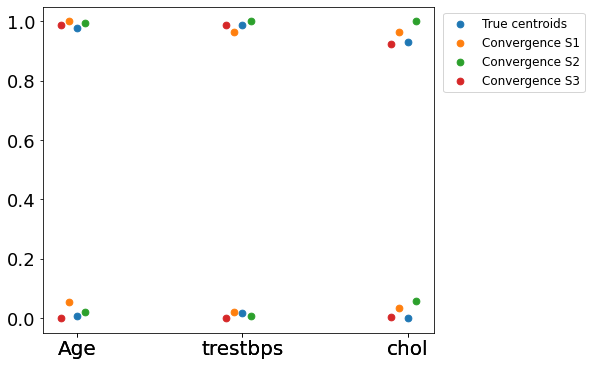
\includegraphics[scale=0.50]{figures/my_cluster_3.png}
\label{fig:cluster_free_3s} 
\end{figure}



%TC:endignore
\begin{table}[htbp]
\centering
 \setlength{\tabcolsep}{7pt} % Default value: 6pt 
 \renewcommand{\arraystretch}{1.35} % Default value: 1
  \captionsetup{justification=centering} 
\caption[Final Data points after convergence of clustering]{Final Data points after convergence; S1, S2 and S3 are the centroids obtained in each silo (S) after convergence; True centroids are the centroids of the true means of all silos (TC)}
\label{tab:datapoints}
\begin{tabular}{lccc}
\toprule
 & Age & trestbps & chol \\
\midrule
S1 & 46.3 , 61.1 & 121.1 , 148.9 & 218.9 , 300.8 \\
S2  & 45.8 , 61.0 & 120.7 , 149.9 & 220.9 , 304.0 \\
S3 & 45.5 , 61.0 & 120.5 , 149.6 & 216.1 , 297.4 \\
TC  & 45.6 , 60.8 & 121.0 , 149.6 & 215.8 , 297.9   \\

\bottomrule
\end{tabular}
\end{table}




%TC:ignore



\begin{figure}[H]
\centering
\captionsetup{justification=centering}
\caption[Clustering for 3 variables with 9 silos]{Clustering for 3 variables with 9 silos and true centroids of the true means (TC); 2 continuous and 1 categorical one hot encoded, The values were normalised for visualisation purposes with MinMax}\label{fig:cluster_mydata_9s} 
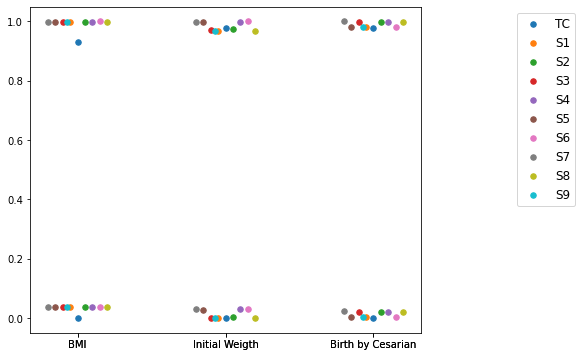
\includegraphics[scale=0.60]{figures/my_cluster_9.png}
\end{figure}
%TC:endignore

As before, the data is in table format in \ref{tab:datapoints_9}.

%%True Centroid & 24.9 , 25.3 & 66.6 , 65.6  & 0.24 , 0.29 \\

\begin{table}[htbp]
\centering
 \setlength{\tabcolsep}{7pt} % Default value: 6pt 
 \renewcommand{\arraystretch}{1.35} % Default value: 1
  \captionsetup{justification=centering} 
\caption{Final Data points after convergence and true centroids of the true means of each silo (TC)}
\label{tab:datapoints_9}
\begin{tabular}{lccc}
\toprule
 & \acs{bmi} & Initial Weight & Birth by Cesarian \\
\midrule
TC & 24.9 , 383.1 & 60.5 , 85.0  & 0 , 1 \\
S1 & 40.1 , 409.4 & 60.4 , 85.0 & 0.96 , -0.04 \\
S2 & 40.1 , 410.4 & 61.7 , 86.3 & 0.99 , -0.01 \\
S3 & 40.0 , 410.4 & 61.9 , 86.5 & 0.96 , -0.04 \\
S4 & 40.6 , 411.3 & 61.9 , 86.5 & 0.96 , -0.04 \\
S5 & 40.0 , 410.4 & 60.5 , 85.1 & 1.0 , 0.0 \\
S6 & 40.1 , 409.3 & 60.4 , 84.9 & 1.0 , 0.0 \\
S7 & 40.7 , 411.3 & 60.5 , 85.0 & 0.96 , -0.04 \\
S8 & 40.0 , 410.4 & 86.5 , 61.9 & 1.0 , 0.0 \\
S9 & 41.0 , 410.4 & 85.0 , 60.4 & 1.0 , 0.0 \\
\bottomrule
\end{tabular}
\end{table}




Then we experimented with categorical variables. Figure \ref{fig:cluster_3_cat} shows the convergence of the silos with proportion data and K-means with that and with K-modes.
\begin{figure}[ht]
\caption{Clustering for 3 variables with 3 silos - (A) categorical variables with  proportion with K-Means and (B)  Categorical with K-modes  }\label{fig:cluster_3_cat} 
  \subcaptionbox*{(A)}[.60\linewidth]{%
    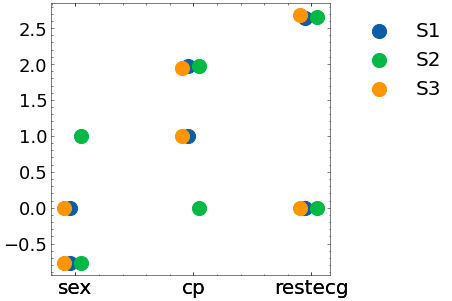
\includegraphics[width=\linewidth]{figures/my_cluster_3_cat.png}%
  }%
  \hfill
  \subcaptionbox*{(B)}[.44\linewidth]{%
    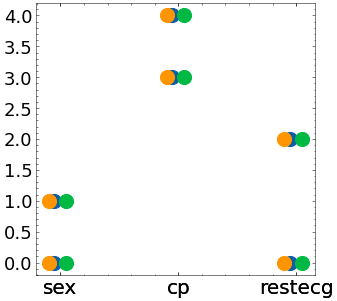
\includegraphics[width=\linewidth]{figures/my_cluster_3_cat_kmodes.png}%
  }
\end{figure}


\subsection{Discussion}
As per the discussion, there are a few issues to be addressed. First as per data preprocessing. In order to cluster be obtained, the null data must be filled out. There are a few strategies to do so. One option is to eliminate records/rows with empty cells or impute data. Either is a possibility, with pros and cons but the capability of having a dataset where no null records are present across several features may be difficult to find in the wild, especially since there are often optional and conditional fields in most Electronic Health Records (EHR). So imputation becomes more interesting, since it enables the usage of the whole dataset, even if biases are introduced.
Mixed types of datasets are also an issue to be aware of. In this case, not only imputation but also encoding a categorical variable is a vital step to take in the preprocessing phase. There are usually two main methods of data encoding, ordinal encoding and binary encoding. The first one keeps a unique column as the original data but maps every category to an increasing natural number. This creates an ordering in the data, often a misrepresentation of reality, not only due to this hierarchy but only because it assumes the differences between ranks of the hierarchy are always the same (1). The second is related to expanding the number of columns into the number of categories and creating 0s and 1s for the category. In machine-learning terms, binary seems more suited to be applied, but for benchmarking purposes, both are below par in terms of interpretability. For categorical data, we found out that K-modes seem to fulfil the requirements in a better way, providing better interpretability and reasoning about the results. However, it should be noted that we applied K-modes in a multivariate fashion and K-means in a univariate fashion.
Given that no percentage is provided, only the mode of the data, we believe it is still hard to get any real insight from the centroids. However, K-modes provides less information, since it only shows the top two categories. Which, for example. binary targets, provide little to no information. However, for larger categorical sets, the information provided could be better. Moreover, the number of centroids pretended could be more important as well. Agreeing on only 1 centroid would render the mode of the data provided by all silos, which could be more interesting.
As for continuous data, the use of real data was insightful, since BMI had a few very big outliers around 300 and 400, which rendered centroids around that data. Even if not all silos had examples of these outliers, the ones that do have, pass that into the remaining. One possible workaround would be an addition of an extra cluster in order to catch possible outliers.
However, this should be addressed in detail and assess how outliers could subvert the data from the silos and how to work around that.

% should be addressed more in focus since it was outside of the scope of this paper
As for the next steps, a few issues could be addressed in depth. Regarding imputation, it could be interesting to understand how imputation, and which methods are more suitable to use for real-world scenarios. If the imputation of variables with a high null percentage influence significantly a centroid formation.
Communication could be important as well. Which action is to be taken when a silo is "down" and does not send information to the remaining. Cluster information should be addressed as well. They need to be agreed upon beforehand in the scope of this paper. But if it could be selected by each silo? Would that be feasible or a convergence could be achieved?
Finally, there is the question if there is the possibility of having leaks of true means across iterations by adversarial learning. At present time, we cannot be sure that the values are totally private, but then again, nothing is.


% abordar na questao a vantagem da privacidade mas que é possivel haver leak dos valores por adervisal learning.

\subsection{Conclusion}
We believe that this work helps create the foundation for exchanging data across healthcare institutions without revealing the true data points. It could be useful for benchmarking and promoting a higher adoption rate.
Even though there are still issues to be addressed, we think that the path is full of possibilities.




% !TeX root = ../thesis.tex

\begin{savequote}[65mm]
    I don't want to insist on it, Dave, but I am incapable of making an error.
    \qauthor{HAL 9000}
    \end{savequote}
    
\chapter{Explore Strategies to Transform Health Data Into Actionable Decisions and Policies}\label{chap:goal3}

\initial{T}his chapter focuses on the practical application of health data in influencing decisions and policies, particularly in the realms of drug evaluation and obstetrics, as detailed in sections \ref{subsec:ipop} and \ref{subsec:obs}.

Section \ref{subsec:ipop} represents an innovative application of causality principles and transparent \ac{ml} models to assess the real-world effectiveness of two groups of breast cancer drugs. Beginning with traditional analysis methods, the study progressively adopts more complex techniques, including \ac{iptw} to enhance the comparative assessment of these treatments. This approach exemplifies how health data, analysed through advanced methodologies, can influence drug policy and treatment choices in clinical settings.

Section \ref{subsec:obs} is an extension of research in distributed data mechanisms (referenced in section \ref{subsec:distributed}), uses \ac{ml} to develop a \ac{cdss} designed to assist in evaluating \ac{cs}. The system's interoperability and its focus on supporting subpar evaluation of \ac{cs} demonstrate the utilization of health data in creating tools that aid in decision-making processes in obstetrics. This section underscores the importance of applying health data analytics in real-time clinical environments to inform decisions and shape obstetrical policies.



\section{How Can We Leverage Data to Assess Treatment Efficacy?}\label{subsec:ipop}
This section is based on the paper entitled "Comparative Analysis of Palbociclib and Ribociclib: A real world data and Propensity Score-Adjusted Evaluation with endocrine therapy" \cite{coutinho-almeidaCDK4InhibitorsEndocrine2024}. This was a method of applying the knowledge of causality and transparent \ac{ml} models in order to assess the real-world effect of two drugs for breast cancer. We started with traditional analysis and then moved to a more complex approach, using \ac{iptw} methods in order to further compare treatments.
    
    
\subsection{Introduction}
    Currently, metastatic breast cancer is difficult to treat. Patients with \ac{hr+} and \ac{her2} breast cancer, the most common subtype, typically undergo \ac{et}. Therefore, new treatments can be very useful in improving quality of life, reducing toxicity, and decreasing scenarios of hormonal resistance.
Medications from the group of \ac{cdk46i} appear as a potential improvement in the therapeutic approach to advanced breast cancer. Within this group, there are palbociclib, ribociclib and abemaciclib. \ac{cdk46} are responsible for regulating the cell cycle at the transition between the G1 and S phases. In many neoplasms, this cycle is deregulated, and it promotes uncontrolled cell proliferation. It is then possible for these medications to have better effectiveness. These medications were approved by INFARMED, I.P. after an analysis of the therapeutic value they offer. This decision was made based on data provided by clinical trials done with these medications. The MONALEESA \cite{hortobagyiUpdatedResultsMONALEESA22018, slamonPhaseIIIRandomized2018, tripathyRibociclibEndocrineTherapy2018} studies were used for ribociclib, PALOMA \cite{vermaPalbociclibCombinationFulvestrant2016, rugoImpactPalbociclibLetrozole2018, finnCyclindependentKinaseInhibitor2015a} for palbociclib, and MONARCH \cite{goetzMONARCHAbemaciclibInitial2017, sledgeMONARCHAbemaciclibCombination2017} for abemaciclib.
These studies focused on testing the hypothesis of treating \ac{cdk46i} in combination with an aromatase inhibitor or fulvestrant as an alternative to the gold standard. In these research findings, it was determined that there was a notable enhancement in effectiveness, supporting their application in clinical practice.
However, this evaluation was based on clinical trials with very specific inclusion and exclusion criteria and in a highly controlled environment. It is then vital to study how these new molecules compare to current practice in terms of treatment effectiveness in a real-world setting. In the meticulously controlled setting of clinical trials, patient selection often skews towards relatively healthier individuals with fewer comorbidities. However, in real-world clinical practice, patients present a diverse range of health profiles, co-existing illnesses, and medication histories that may influence drug efficacy and safety. Real-world data, drawn from electronic health records, insurance claims databases, and patient registries, offers the advantage of reflecting a more heterogeneous patient population, thus potentially uncovering insights not readily apparent in clinical trial settings. Understanding the effectiveness and safety of \ac{cdk46i} in real-world conditions is crucial for tailoring more individualized treatment regimens, optimizing outcomes, and enhancing the quality of life for patients with \ac{hr+}, \ac{her2} breast cancer \cite{harbeckCDK4InhibitorsHR2021}. Nevertheless, observational studies have inherent limitations, such as confounding by indication, which can lead to biased estimates of treatment effects. To tackle this, there are causality-based assessments that can be employed in order to better estimate the causal effects of treatments.
Incorporating statistical techniques like \ac{iptw} can play an essential role in enhancing the quality of real-world evidence by accounting for treatment selection bias and balancing observed covariates between treatment groups. \ac{iptw}, grounded in the framework of causal inference, allows for the mimicking of a randomized control trial-like setting within observational studies. By assigning weights to individual patients based on their propensity scores—the likelihood of receiving a particular treatment given a set of observed characteristics—analyses can achieve a balance between different treatment arms, thereby reducing bias and confounding factors. Establishing causality, rather than mere association, is vital for the robust interpretation of real-world data. As we strive to understand the long-term impact, efficacy, and safety of \ac{cdk46i} in \ac{hr+}, \ac{her2} breast cancer, the rigorous application of \ac{iptw} and causal inference methods can substantially augment the validity of real-world findings, making them a more reliable basis for clinical decision-making \cite{austinIntroductionPropensityScore2011,austinUsePropensityScore2014}
So in this paper, we propose:
\begin{itemize}
    \item To compare the effectiveness of the \ac{cdk46i} drug class in terms of  \ac{pfs}  and \ac{os} \ac{os};

    \item To assess the Hazard Ratio of using the \ac{cdk46i} drug class in terms of \ac{pfs} and \ac{os}.
    
    \item  To compare the effectiveness of \ac{cdk46i} in combination with letrozole or fulvestrant with the previous standard of care in terms of \ac{pfs} and \ac{os} in patients with \ac{hr+}, \ac{her2} advanced breast cancer with bone only metastasis.

    \item To assess the differences in effectiveness between the three \ac{cdk46i} in combination with letrozole or fulvestrant in terms of \ac{pfs} and \ac{os} with causality principles in mind, especially the counterfactual theory and \ac{iptw}.
    
\end{itemize}

    \subsection{Materials \& Methods}
    

\subsection{Study Design}

This retrospective study was designed in 2022. The study aimed to evaluate the clinical benefit and long-term survival of patients with \ac{hr+}/\ac{her2} that started treatment with \ac{cdk46i} plus \ac{et} in different lines of treatment between the 14th of March 2017 and the 31st of December 2021. The follow-up period was set until June 2022. Inclusion criteria: women and men, \ac{hr+} and \ac{her2} in the primary tumor or metastatic site after biopsy. Exclusion criteria: Patients that had only one ambulatory medication, and patients involved in clinical trials, diagnosed with other neoplasms or with active treatment during the study period. The control group was defined by a population of patients, that were treated with hormone therapy as first-line (due to bone metastases only) between 2015 and 13 of match 2017.
The evaluation of effectiveness will involve \ac{os} and progression-free analysis. We will compare the two different \ac{cdk46i} in terms of effectiveness in real-world patients and will also compare the effectiveness of this class combined with \ac{et} against traditional \ac{et}.


\subsection{Data collection}
All data were collected from medical and administrative records from baseline to last visit or death. The data was collected from Instituto Português de Oncologia – Porto (IPO-P). Table 1 shows a comparison between the groups.
Data included for population treated with \ac{cdk46i} plus \ac{et}: demographic information, age at first diagnosis and age at the beginning of treatment, clinical characteristics and performance status by  \ac{ecog}, treatment line and treatment schema - CDK4/6 inhibitor and \ac{et}, stage of cancer, site of metastases (bone, soft tissue, visceral, central nervous system with or without another site).
Data included for the population treated with \ac{et} as first-line: demographic information, age at first diagnosis and age at the beginning of treatment, clinical characteristics and performance status by  \ac{ecog}, stage of the cancer.
For comparison purposes, we used palbociclib and ribociclib since we had a small number of patients treated with abemaciclib (12).

 
\begin{table}
\caption{Descriptive statistics of \ac{cdk46i} group and \ac{et} group. The Drug/combination refers to the actual drug or the combination for CDK4/6}
\centering
\label{tab:stats_ipop_cdk}

\begin{tabular}[t]{llll}
\toprule
  &\ac{et}& Palbociclib & Ribociclib\\
\midrule
 & (N=43) & (N=246) & (N=106)\\
\addlinespace[0.3em]
\multicolumn{4}{l}{\textbf{Age at treatment start}}\\
\hspace{1em}Mean (SD) & 60.1 (12.4) & 59.2 (11.7) & 58.2 (10.7)\\
\hspace{1em}Median [Min, Max] & 62.0 [34.0, 85.0] & 60.0 [28.0, 84.0] & 58.0 [32.0, 79.0]\\
\addlinespace[0.3em]
\multicolumn{4}{l}{\textbf{Bone Only metastases}}\\
\hspace{1em}No & NA & 161 (65\%) & 74 (70\%)\\
\hspace{1em}Yes & NA & 85 (35\%) & 32 (30\%)\\
\hspace{1em}Missing & 43 (100\%) & 0 (0\%) & 0 \vphantom{1} (0\%)\\
\addlinespace[0.3em]
\multicolumn{4}{l}{\textbf{Visceral metastasis}}\\
\hspace{1em}No & NA & 121 (49\%) & 49 (46\%)\\
\hspace{1em}Yes & NA & 125 (51\%) & 57 (54\%)\\
\hspace{1em}Missing & 43 (100\%) & 0 (0\%) & 0 (0\%)\\
\addlinespace[0.3em]
\multicolumn{4}{l}{\textbf{Stage}}\\
\hspace{1em}I & 3 (7\%) & 22 (9\%) & 7 (7\%)\\
\hspace{1em}II & 20 (47\%) & 75 (30\%) & 22 (21\%)\\
\hspace{1em}III & 11 (26\%) & 74 (30\%) & 18 (17\%)\\
\hspace{1em}IV & 2 (5\%) & 65 (26\%) & 46 (43\%)\\
\hspace{1em}Missing & 7 (16.3\%) & 10 (4.1\%) & 13 (12.3\%)\\
\addlinespace[0.3em]
\multicolumn{4}{l}{\textbf{Drug/Combination}}\\
\hspace{1em}Anastrozol & 3 (7\%) & NA & NA\\
\hspace{1em}Exemestane & 4 (9\%) & NA & NA\\
\hspace{1em}Fulvestrant & 5 (12\%) & 180 (73\%) & 10 (9\%)\\
\hspace{1em}Letrozol & 31 (72\%) & 66 (27\%) & 96 (91\%)\\
\bottomrule
\end{tabular}

\end{table}




\subsection{Statistical Analysis}
%copied
R was used for statistical analysis. Demographic, clinical characteristics and side effects were analyzed using descriptive statistics (count, percentages and median/range). Kaplan–Meier test was used to determine the median \ac{pfs} and \ac{os} in the entire population and subgroups. Log-rank test was used for comparisons of \ac{pfs} and \ac{os} among different subgroups. Cox Regression was used to assess feature importance and impact. All statistical tests were two-sided, and the significance level was 0.05. The evaluation of the proportional hazards assumptions was done by \textit{Schoenfeld} residues analysis.
We applied propensity score weights to achieve a more robust comparison between the two groups of CDK4\/6i. We used the existence of visceral metastases, treatment line, age at treatment start, and stage. We used the WeightIt package for R \cite{WeightIt}. We applied the weights to the Kaplan-Meier curves and to the Cox Regression. We applied the weights to get the \ac{ate} which is $E[Y_i(1)-Y_i(0)]$, the average effect of moving an entire population from untreated to treated, or from one drug to the other. Weights were used instead of matching since it is more suited for calculating \ac{ate} and the need to preserve the sample size since it is already small from the start. The formula for calculating the weights was through propensity score weighting with \ac{glm}. Multiple comparisons were done with the \ac{bh} method. 



%Pretende-se que \ac{os} dados venham do Instituto Português de Oncologia – Porto (IPO-P). Pretende-se utilizar a base de dados do hospital dos últimos 5 anos.
%O estudo será registado e respeitará todos \ac{os} requisitos éticos de aprovação a comissão de ética de cada instituição participante. Caso a instituição tenha um encarregado de Proteção de Dados (EPD), este será contactado a fim de dar seu parecer, e caso necessário, a sua opinião para melhorar possíveis pontos relacionados à segurança de dados.

%The goal is to identify the clinical or biological variables that have the most impact on a specific outcome. To achieve this, considering the statistical models found, we can model things in terms of time series or survival trees to group outcomes and the clusters found. With this, we can analyze the effectiveness of the clinical course, probabilities of recurrence, or survival rates by subgroup. These models and relationships can form the basis of a clinical decision support system and can be crucial for making better healthcare decisions.

%Some of the techniques used are unsupervised techniques such as k-means, DBSCAN, or hierarchical clustering.
%The goal is to identify the clinical or biological variables that have the most impact on a specific outcome. To achieve this, considering the statistical models found, we can model things in terms of time series or survival trees to group outcomes and the clusters found. With this, we can analyze the effectiveness of the clinical course, probabilities of recurrence, or survival rates by subgroup. These models and relationships can form the basis of a clinical decision support system and can be crucial for making better healthcare decisions.

%Some of the techniques used are unsupervised techniques such as k-means, DBSCAN, or hierarchical clustering.

    \subsection{Results}
    The median \ac{os} in the entire population treated with \ac{cdk46i} was 46 months (95\% CI 39.4–55.6). Median \ac{pfs} was 20.1 months (95\% CI 18.3–24.2). Following this, we compared Palbociclib and ribociclib only as first-line treatments. We found that regarding \ac{os}, there is no significant difference between the two, but ribociclib is significantly better in terms of \ac{pfs} (\textit{P} value $\le$ 0.001) (Figure \ref{fig:interest}). Additionally, we compared the same \ac{cdk46i} with letrozole as a combination only (PAL-LT and RIB-LT). Regarding this scenario, we found out that both were similar in terms of \ac{os} and \ac{pfs}.


\begin{figure}[ht]
  \caption[Survival curves for Palbociclib and Ribociclib (1st line)]{Survival curves for Palbociclib and Ribociclib (1st line) - \ac{pfs} and \ac{os}}\label{fig:interest} 
  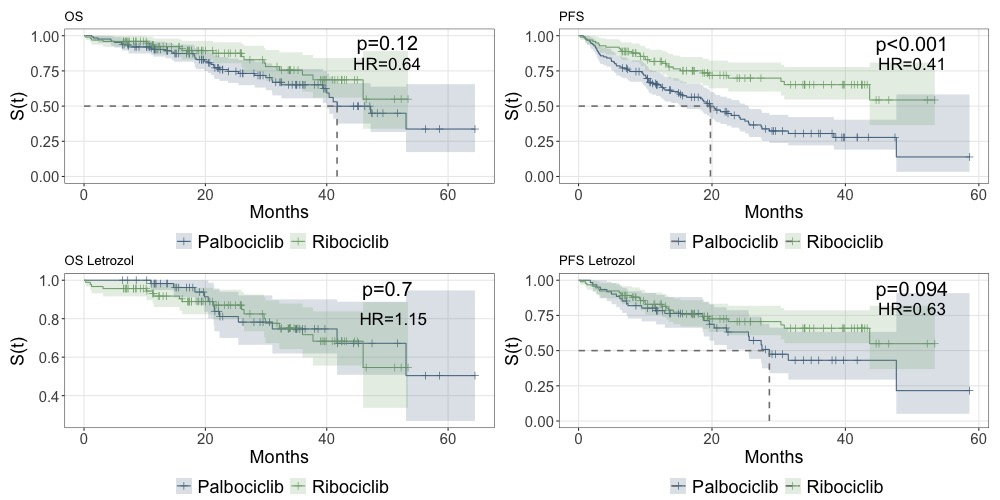
\includegraphics[scale=0.45]{figures/interest_curve_both.jpeg}%

\end{figure}


We then compared both with a cox regression, where \ac{os} shows no significant difference between palbociclib and ribociclib when adjusted to the stage, visceral metastases, age, treatment line, combination and \ac{ecog}. The proportional hazards' assumption was confirmed with \textit{P} values all over 0.10.
\begin{table}[ht]
  \centering
  \caption[Cox Regression with palbociclib and Ribociclib - \acs{pfs} and \acs{os}]{Cox Regression with palbociclib and Ribociclib - \ac{pfs} and \ac{os}}\label{tab:cox} 
  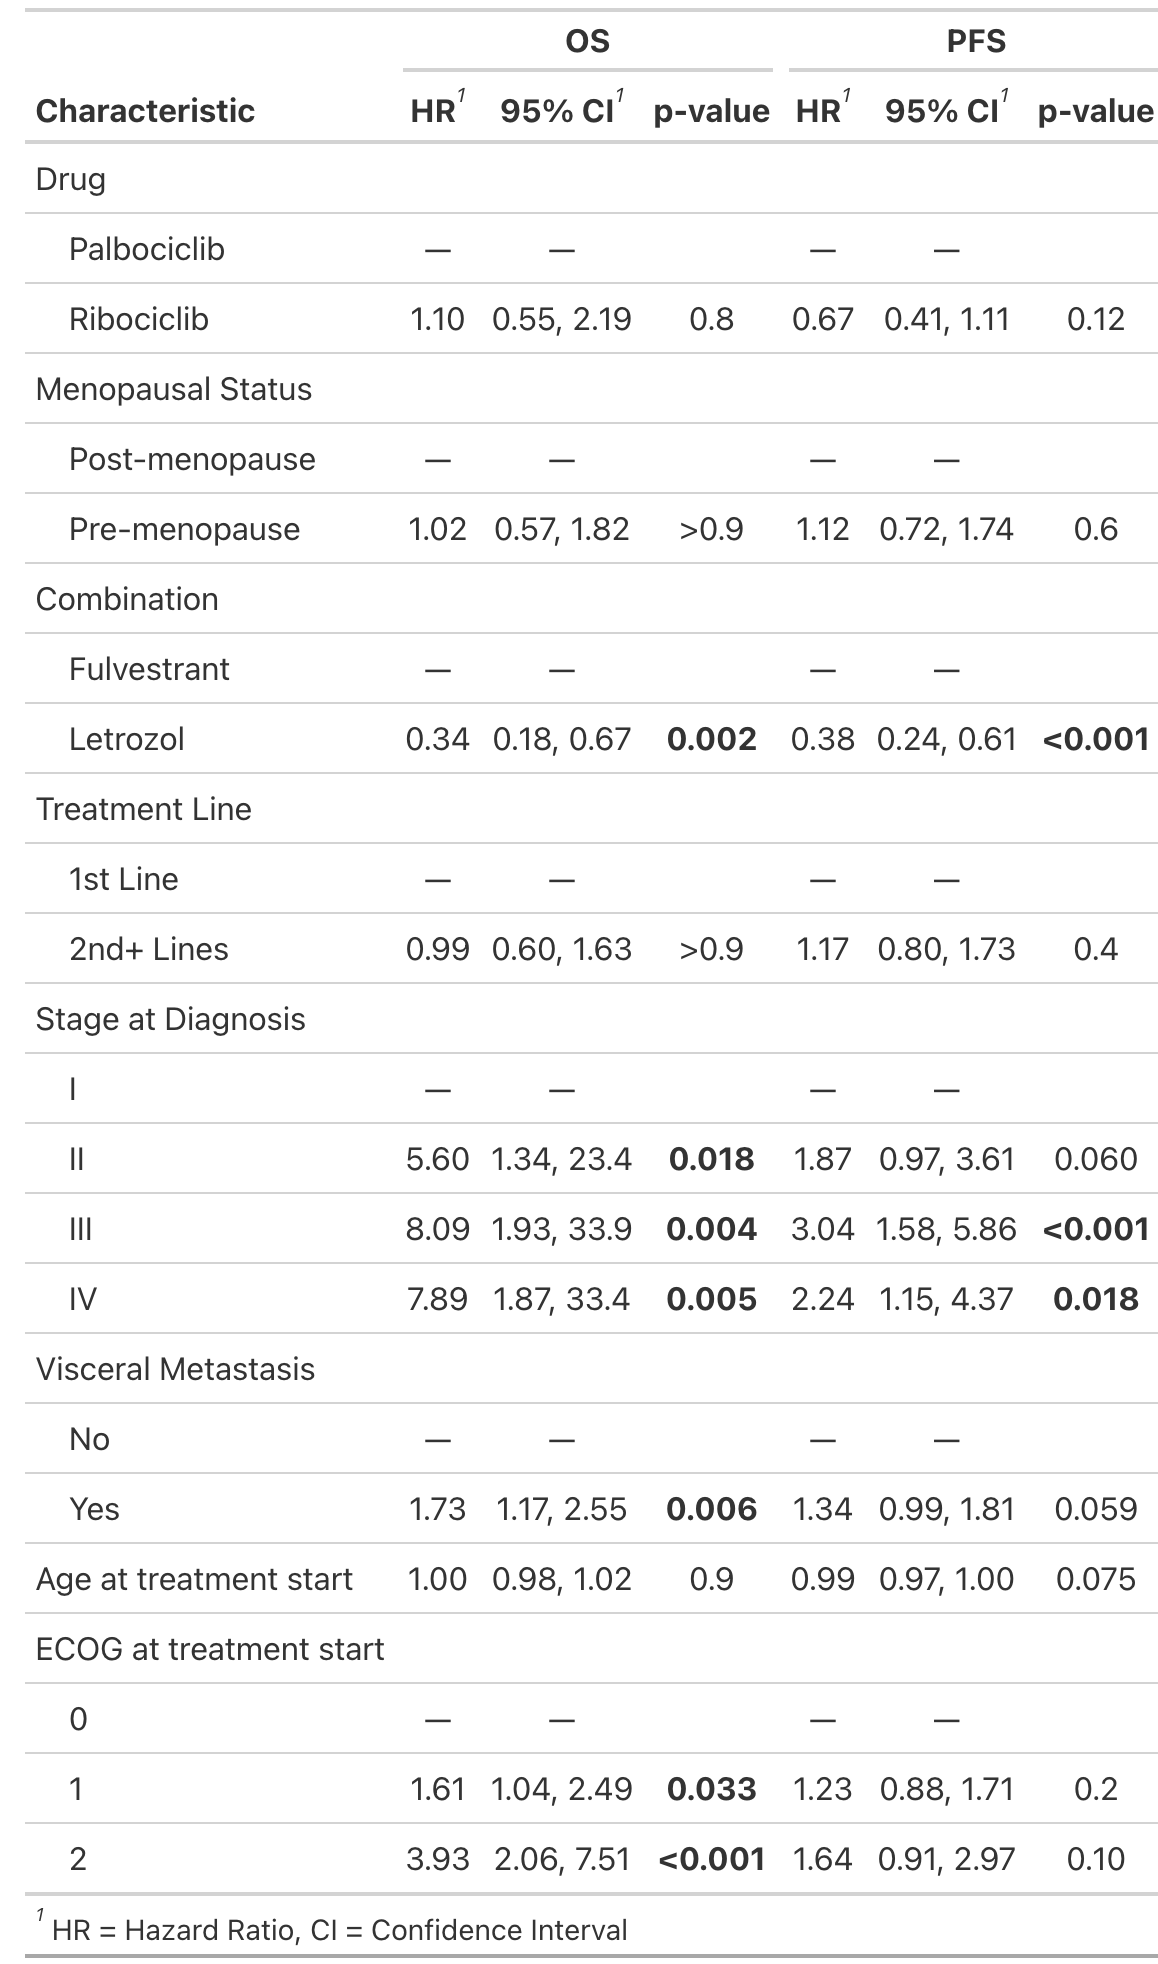
\includegraphics[scale=0.20]{figures/cox_both.png}%

\end{table}

When comparing \ac{et} with \ac{cdk46i} as first-line treatment (figure \ref{fig:grouped}). For this study we only compared patients with bone only metastasis. When comparing both \ac{cdk46i} combined with Fulvestrant or letrozole, we see that  Ribociclib (RIB+LT/FUL) is significantly better for \ac{pfs} (\textit{P} value $\le$ 0.001 \ac{hr}=0.21) but not \ac{os}. For Palbociclib as the first line with Fulvestrant or letrozole (PAL+LT/FUL), we see that there is no significant difference in terms of \ac{pfs} and \ac{os} (\textit{P}=0.57 and 0.51). We also applied the same analysis but comparing only the letrozole combination with letrozole alone (PAL-LT/RIB-LT vs LT). We found that both ribociclib and palbociclib are significantly better in terms of \ac{pfs} (\ac{hr} 0.65 for palbociclib and 0.27 for ribociclib) but not \ac{os}.
\begin{figure}[ht]
  \centering

  \caption[Survival curves (\acs{os} and \acs{pfs}) comparing \acl{et} to \acl{cdk46i} combined with fulvestrant or letrozole as 1st line.]{Survival curves (\ac{os} and \ac{pfs}) comparing \ac{et} to \ac{cdk46i} combined with fulvestrant or letrozole as 1st line. First row is \ac{cdk46i} combined fulvestrant or letrozole vs fulvestrant or letrozole. Second row is \ac{cdk46i} combined with letrozole vs letrozole alone. \textit{P} values shown as pairwise vs. ET. }\label{fig:grouped} 
  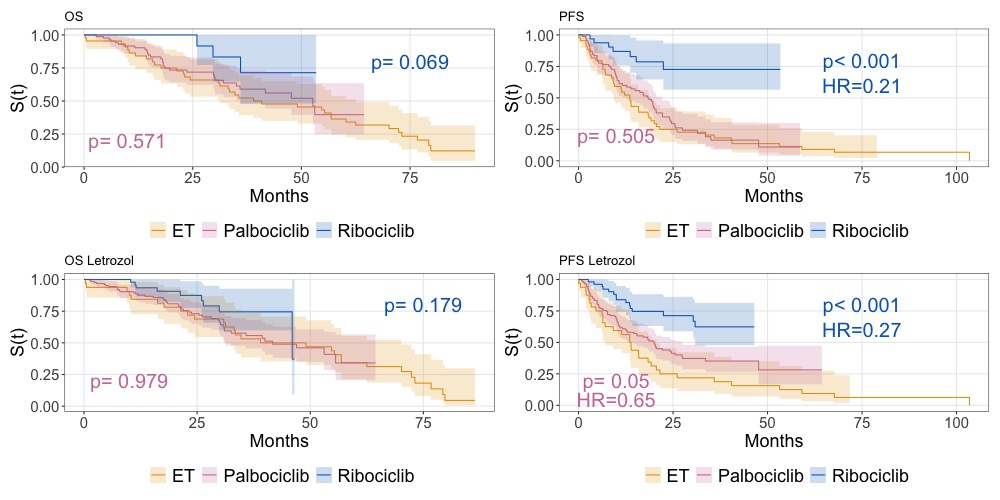
\includegraphics[scale=0.42]{figures/grouped_curve_both.jpeg}%

\end{figure}

When comparing palbociclib and ribociclib adjusted for \ac{ate} weights, we found a different scenario from previous assessments. There is a significant difference between the two in terms of \ac{os} (figure \ref{fig:propensity}). The weights were calculated as stated in the methods section.


\begin{figure}[ht]
  \centering

  \caption{Comparison of palbociclib and ribociclib survival curves adjusted for propensity scores}\label{fig:propensity} 
  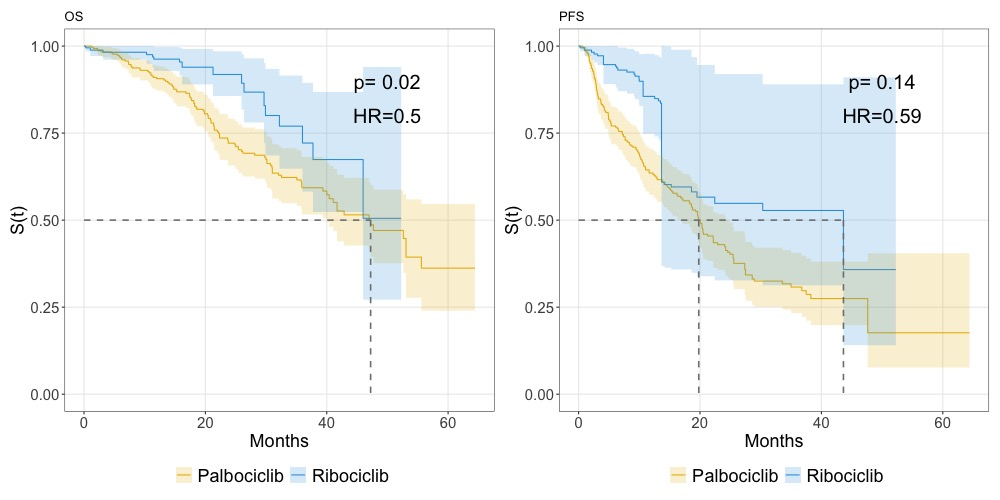
\includegraphics[scale=0.42]{figures/propensity_score_both.jpeg}%

\end{figure}

The Cox regression adjusted for the variables and with the weights applied to render an \ac{hr}=0.55 [95\% CI 0.28-1.09;\textit{P}=0.086] for \ac{os}. The \ac{hr} for \ac{pfs} is 0.56 [95\% CI 0.32-1;\textit{P}=0.05].
    \subsection{Discussion}
    The aim of this study was to evaluate the real-world use of palbociclib and ribociclib in combination with \ac{et} for \ac{hr+}/\ac{her2} and compare this drug class with traditional \ac{et}. Few real-world evidence studies of palbociclib and ribociclib used in daily clinical practice have been published identifying clinical benefit, patient profile, and sequencing of treatment, with even less evidence for the Portuguese population.

When comparing with clinical trials, regarding patient profile, in our study, 51\% had visceral metastasis and 35\% had bone-only metastases compared with 49\% and 38\% in PALOMA-2, and 60\% and 25\% in PALOMA-3, respectively \cite{rugoImpactPalbociclibLetrozole2018,cristofanilliFulvestrantPalbociclibFulvestrant2016a}.
As for ribociclib and bone-only metastases, MONALEESA-7 \cite{tripathyRibociclibEndocrineTherapy2018} has 24\% and MONALEESA-2 has 40\% \cite{hortobagyiUpdatedResultsMONALEESA22018} and our study has 30\%. Regarding menopausal status, our study has 20\% premenopausal and 80\% postmenopausal. 



Of note, the range of median \ac{pfs} for first-line palbociclib was 15.5–25.5 months, which is shorter than 27.6 months observed in a post hoc analysis of the PALOMA-2 clinical trial with extended follow-up \cite{rugoImpactPalbociclibLetrozole2018}, but in line with RWE studies (13.3–20.2 months) \cite{harbeckCDK4InhibitorsHR2021}. When assessed with only letrozole as a combination, the median \ac{pfs} increased to 28.6 months [95\% CI 25.5-not reached]. Additionally, analysing the postmenopausal women subgroup, palbociclib showed a median \ac{pfs} of 16.3 months [95\% CI 12.9 -20]. Furthering analysis of the postmenopausal and with letrozole, the median was 47.6 months [95\% 25.6-2–not reached].

As for ribociclib, median survival time was not reached whether in \ac{os} and \ac{pfs}. So we can at least say that the median \ac{pfs} is longer than 50 months. This is longer than the median \ac{pfs} of 23.8 months (95\% CI 19.2–not reached) reported in the MONALEESA-7 trial \cite{tripathyRibociclibEndocrineTherapy2018} and longer than  25.3 months (95\% CI 23.0–30.3) in the MONALEESA-2 trial \cite{hortobagyiUpdatedResultsMONALEESA22018}. Regarding the subgroup analysis of postmenopausal women, we noticed that the median was not reached for women treated with ribociclib and fulvestrant or letrozole (RIB-LT/FUL) and postmenopausal women treated with ribociclib in combination with letrozole (RIB-LT).

When directly comparing ribociclib and palbociclib without any adjustments, one might deduce that ribociclib is superior to palbociclib. However, after adjusting for confounding variables, there is no significant difference between the two inhibitors in terms of \ac{pfs} or \ac{os} as indicated in table 2. This observation is further corroborated by the lower plots in figure 1, where even a subgroup analysis of \ac{cdk46i} combined solely with letrozole reveals non-significant difference between the two.

In the first-line comparison, the analysis of \ac{os} outcomes reveals no substantial difference between \ac{et} alone and the combination of \ac{cdk46i} with \ac{et}, irrespective of whether the \ac{cdk46i} are administered with fulvestrant or letrozole  (PAL-LT/FUL vs LT/FUL; \textit{P}=0.57 | RIB-LT/FUL vs LT/FUL \textit{P}=0.069) or exclusively with letrozole (PAL-LT vs LT; p = 0.979 | RIB-LT vs LT; \textit{P}=0.179)(figure \ref{fig:grouped} left). With respect to \ac{pfs}, ribociclib demonstrates superior efficacy when compared its combination with any of the adjuvants to these adjuvants alone (RIB-LT/FUL vs LT/FUL; \ac{hr}=0.21) as well as when combined only with letrozole (RIB-LT vs LT; \ac{hr}=0.27). Additionally, palbociclib exhibits significant improvement in \ac{pfs} when combined with letrozole  (PAL-LT vs LT; \ac{hr}=0.65) (figure \ref{fig:grouped} right).
When comparing with propensity scores weighting, we found out that ribociclib is significantly better than palbociclib for \ac{pfs} and \ac{os}, providing a median \ac{os} of over 40 months and median \ac{pfs} of around 42 months. Adjusted for the weighted variables, Ribociclib is not significantly better for \ac{pfs}, but has a \textit{P} value of 0.013 for \ac{os} with an \ac{hr} of 0.48. However, the Cox regression adjusted for variables and weights are not significant, even when the \textit{P} value for \ac{pfs} is 0.05. This suggests that a more in depth analysis may be necessary.



    \subsection{Conclusion}
    In conclusion, our findings underscore the efficacy of \ac{cdk46i} in real-world settings. We can confidently affirm the impact of Ribociclib on \ac{pfs}. This assertion aligns with clinical trial outcomes and real-world data further substantiates these findings. However, we cannot do the same for \ac{os}. Our results indicate that Ribociclib combined with letrozole or fulvestrant when compared to both is not superior to these alternatives used alone. The same happens when comparing ribociclib combined with letrozole with letrozole alone. 
However, we cannot do so for Palbociclib. Palbociclib combined with fulvestrant or letrozole was not significantly better than letrozole or fulvestrant alone for \ac{pfs} nor \ac{os}. This is something interesting that we want to follow up with.
Delving deeper into the characteristics of the patient population, including safety profiles, economic implications, and quality of life metrics, would be insightful. Additionally, a thorough examination of biomarkers within the population could offer invaluable insights. Finally, extending the follow-up period would be beneficial as well. We intend to explore these facets in subsequent publications.
It’s imperative to note that our data is sourced from a singular institution, limiting the capability of generalization of our results to a broader population. Nonetheless, we posit that this study lays a foundational groundwork for future research in this domain. While our evidence is rooted in observational data, and we’ve made adjustments for known confounders, the potential for residual confounding remains. Although the use of propensity score matching enhances the comparative robustness between the groups, the presence of unmeasured confounders cannot be entirely ruled out. Furthermore, the small sample size of our study limits the statistical power of our findings. For next steps we aim to further analyse the clinical variables that have an impact on the outcome of the combination of CDK4/6 with fulvestrant or letrozole and these drugs used alone in order to infer pharmaeconomic implications and possible profiles of patient that would not benefit from this combination which would be vital for economic reasons and to apply in countries with low access to these drugs.
    
    
    \section{How Can We Leverage Data to Create Clinical Decision Support Systems?}\label{subsec:obs}
    This section is based on the paper entitled "Machine-learning in Obstetrics: FHIR-based Support System for predicting delivery type" \cite{coutinho-almeidaFastHealthcareInteroperability2024c}. This work was in part a result of the work in section \ref{subsec:distributed}. While testing for distributed mechanisms, we kind of felt that some evaluation metrics were inspiring to pursue this further. We built a \ac{cdss} system that is interoperable and aims to provide support for subpar evaluation of a \ac{cs}.
    
    \subsection{Introduction}
    The ability to provide care to both women and newborns during delivery is one of the most important aspects of healthcare and is often used as a metric to assess healthcare as a whole across different countries.
\acp{cs} are one of the most important aspects of delivering babies since it has a considerable impact on the mother's health and well-being. Despite this type of procedure increasing over the last few years, it is still illusive the reasons behind such events. Reports from 2016 suggest that this increment is a global phenomenon, being that from 1990 to 2014, this type of delivery almost increases by 3-fold from 6.7\% to 19.1\% \cite{betranIncreasingTrendCaesarean2016,chenNonClinicalInterventions2018}. Some of these impacts, being more prone to investigation in the last years, including the risk of infection, haemorrhage, organ injury and complications related to the use of anaesthesia or blood transfusion \cite{caesereanrisk1,caesereanrisk2}.
There is also a higher risk of complications in subsequent pregnancies like uterine rupture, abnormal placental implantation and the need for hysterectomy \cite{caesereanrisk3,caesereanrisk4}. As for the infant, \acp{cs} include the risk of respiratory problems, asthma and obesity in childhood \cite{caesereanrisk3}.
Facing this, in 2015, \ac{who} released a statement regarding \acp{cs} rates. Even when other complications could not be totally assessed, it was concluded that \ac{cs} rates higher than 10\% were not associated with a reduction in maternal or newborn mortality \cite{worldhealthorganizationhumanreproductionprogramme10april2015WHOStatementCaesarean2015}.

Since there is no evidence that this type of procedure is beneficial for women or babies when there is no clear need for it, the focus on filtering such cases is important \cite{chenNonClinicalInterventions2018}.
Moreover, particularly in Portugal, \acp{cs} are used as a way of financing healthcare institutions. This was implemented as a strategy of decreasing \acp{cs} across the country. A committee was created especially with the purpose of reducing the percentage of \acp{cs} nationally. One of the actions taken along this creation was the reduction of government funding for hospitals with rates of \acp{cs} above 25\%.
In 2020, the number of \acp{cs} in Portugal is about 36.3\%. Almost at the all-time high of 36.9\% in 2009 \cite{pordatacesarianas}.
So, lowering the proportion of \ac{cs} can provide health and financial benefits to institutions and populations alike. With this in mind, we developed a  machine-learning algorithm-based support system to assist clinical teams to detect cases of potentially unnecessary \acp{cs} for analysis. So in this paper, we propose:
\begin{myitemize}
    \item help to provide a method of bringing to the discussion of clinical staff possible less than optimal care regarding deliveries;
    \item elaborates on how clinical decision support systems can be developed using interoperability standards;
    \item understand, based on the gathered data, which are the more impacting features for predicting delivery type outcome;
    \item open a research path regarding the evaluation of this type of clinical decision support system prior to the delivery;
    \item Perform a concise economic analysis to assess the potential financial impact of implementing the proposed clinical decision support tool.

\end{myitemize}
    \subsection{Rationale and Related Work}
    Regarding the related work, several teams already tackled the potential of predicting the delivery type before birth. However, we believe that creating such a system may have a huge impact on the clinical team, patient and family regarding expectations. For such a system to be possible to enter clinical practice safely, as we hope this one does, several tests and evaluations should be done before going live.
On the other hand, we are aiming for a \textit{post-partum} analysis in order to signalise potential sub-optimal decisions so the clinical teams can evaluate the case afterwards, and hopefully, learn about what could have been done better.
Works and studies on this matter have been done before, related to second opinions in the healthcare practice regarding the decision of the \ac{cs} \cite{mandatorysecondopinion} and the implementation of clinical guidelines help as well \cite{reducingcaeresan}. We hope to provide support to help teams go in this direction.

Nevertheless, in the literature, there are works related to predicting a successful vaginal birth after a previous \ac{cs}, like the work of Lipschuetz et al., \cite{lipschuetzPredictionVaginalBirth2020} where a gradient boosting method was used to predict such event using prenatal data to do so. Grobman et al., \cite{grobman_development_2007} did similar work with a multivariable logistic regression model.
There was also the usage of different modalities of data for predicting delivery type. The work of Fergus et al. \cite{fergusClassificationCaesareanSection2017} introduces a method of predicting delivery type using the fetal heart rate signals. Similarly, the work from Saleem et al. \cite{saleemStrategyClassificationVaginal2019a} proposes a method of predicting delivery type using interactions between fetal heart rate and maternal uterine contraction.
Finally, there are also works that focus on predicting delivery mode before childbirth like the work of Ullah et al. \cite{ullah_reliable_2021} where a boosting algorithm was used in order to predict delivery mode with enriched datasets. Also the work of Gimovsky et al.  \cite{gimovskyBenchmarkingCesareanDelivery} where decision trees were introduced  to predict \acp{cs} by physician group. \\
However, as far as we know, there was no model tested (even in a controlled setting) in clinical practice, with no interoperable format of communication like Fast Healthcare Interoperability Resources (FHIR) or employed to \textit{post-partum} setting and finally, none with real-world data related with Portuguese hospital, making that our paper could be a novelty under very different dimensions.


%---predict c-section


    \subsection{Methods}
    \subsubsection{Clinical Comparison}
The clinical comparison was performed by sending questionnaires to clinicians with a relationship with obstetrics in order to assess 10 patients, with only access to the variables used by the model and to answer three questions for each. The first was to give a score from 1-10 of how likely that patient would give birth through C-section, then to select the feature/variable that most influenced the decision and which feature they would require to make a better assessment. We sent the questionnaire to 20 people and obtained 6 answers, totaling 60 patient assessments. For these 10 patients, we also predicted the delivery type using our model in order to compare it with the clinicians’ answers. These patients were new and were not seen by the model during the training phase.

\subsubsection{Analysis}

%We wrote all of the code in Python 3.9.7 with the usage of the \textit{scikit-learn} library \cite{scikit-learn}. All null representations were standardized. Data was prepossessed with the removal of features with high missing rates ($>$ 90\% overall). All missing value representations were standardized. The imputation process was done using the \ac{knn} imputation method (for continuous variables) or a new category (NULLIMP) for categorical variables. 
%For this purpose, the Birth Type was reduced to binary. All assisted birth were merged into vaginal birth and \ac{cs} remained as the other class. Procedures and diagnosis were also used and were encoded as binary features, we took the time to analyse each one of them in order to avoid leakage since there were procedures obviously related to \acp{cs} and vaginal deliveries.
%Feature creation was done through the free-text variable relating to the medication prescribed. Features were collected from it and converted into \ac{atc} Classification Group level 4, which stands for chemical subgroups. We also created some new features from data in the dataset, namely new categories related to the labour and condition of the baby.
%Also, a few data quality issues were addressed, like impossible values that were transformed into null. In this category, the main issues were \ac{bmi}/Weight and gestational age.
%Finally, only a few columns were selected. We used a mixture of surveying the literature and the feature with greater correlation with the outcome.
%The models tested were Logistic Regression, Decision Tree, Random Forest, 3 different Boosting methods (as implemented by \ac{xgboost}, \ac{lightgbm} and \textit{scikit-learn}) and a linear model based on Stochastic Gradient Descent.
%The evaluation was done with repeated stratified cross-validation with 10 splits and 2 repetitions.   
%The API for serving the prediction model was developed with FastAPI.

%Finally, a clinical evaluation was carried out with questionnaires sent to several obstetrics specialists in order to assess the validity and possible impact of the model.



We obtained full approval from the ethics committee before commencing the study, as detailed in the 'Ethics Approval and Consent to Participate' subsection. The need for informed consent was waived by the ethics committee. All null representations were standardized. Data were prepossessed by removing features with high missing rates (>90\% overall). The imputation process was performed using the KNN imputation method (for continuous variables) or a new category (NULLIMP) for categorical variables. Weight was categorized into percentiles defined specifically for Portuguese babies \cite{sousa-santosDevelopmentBirthweightStandard2016}. For the purpose of this study, the Birth Type was reduced to binary. All assisted birth were merged into vaginal birth and C-Section remained as the other class. Procedures and diagnoses were also used and were encoded as binary features, and we took the time to analyze each one of them in order to avoid leakage because there were procedures obviously related to C-sections and vaginal deliveries. Feature creation was performed through the free-text variable related to the prescribed medication. Medicine names were collected from it and converted into Anatomical Therapeutic Chemical (ATC) Classification Group level 4, which represents chemical subgroups. We also created some new features from data in the dataset, namely new categories related to the labor and condition of the baby. In addition, data quality issues were addressed, such as impossible values that were transformed into null values. The main variables affected by data quality were BMI/Weight and gestational age. The data were split into training and test sets in a 0.75:0.25 manner. From the overall datasets which comprised over 200 columns, only a few columns were selected (please see table \ref{tab:delivery_methods} in the results section). We used a mixture of features selected by surveying the literature \cite{irwindaMaternalFetalCharacteristics2021,deramonfernandezPredictionModeDelivery2022,parveenAnalysisCesareanSections2021} and features with a high correlation with the outcome. The tested models were Logistic Regression, Decision Tree, Random Forest, three different Boosting methods (as implemented by XGBoost, LightGBM and scikit learn) and a linear model based on Stochastic Gradient Descent. The evaluation was performed with repeated stratified cross-validation with 10 splits and 2 repetitions, with two full cycles of dividing the training set into 10 equal parts and using 9 as the training set and 1 as the validation set. This rendered table 3. The API for serving the prediction model was developed using FastAPI. We wrote all the code in Python 3.9.7.
    \subsection{Results}
    \subsubsection{The model}
The results are mainly the model that predicts the occurrence of a \ac{cs} or natural delivery. 
The evaluation metrics are present in the table below for the best hyper-parameters found for the training data.

\begin{table}[htbp]
  \centering
  \caption[Performance Metrics in the training set]{Performance Metrics in the training set with mean \ac{auroc} and 95\% \acl{ci}}
  \label{tab:performance_metrics_auc}
  \renewcommand{\arraystretch}{1.5} % Adjust the vertical spacing
  \setlength{\tabcolsep}{12pt} % Adjust the horizontal spacing
  \begin{tabular}{lcc}
    \hline
    \textbf{Metric} & \textbf{AUC} & \textbf{CI 95\%} \\
    \hline
    \ac{xgboost} & 0.8809 & 0.8799, 0.882 \\  
    Decision Tree & 0.8337 & 0.8324, 0.8349 \\
    Logistic Regression & 0.8716 & 0.8706, 0.8726 \\
    AdaBoost & 0.8753 & 0.874, 0.8766 \\ 
    \ac{lightgbm} & 0.8805 & 0.8793, 0.8817 \\ 
    Stochastic Gradient Descent & 0.8704 & 0.8694, 0.8713 \\ 
    Random Forest & 0.8752 & 0.8743, 0.8762 \\  
    \hline
  \end{tabular}
\end{table}



\ac{xgboost} and \ac{lightgbm} were the best-performing algorithms. However, we selected \ac{lightgbm} \cite{lightgbm}. since it is faster and requires less memory. The threshold selected for deploying the model was 0.7457247885715557 which rendered the metrics in the test set like it is shown in table \ref{tab:performance_metrics_threshold}.

\begin{table}[htbp]
  \centering
  \caption{Performance Metrics in the test set with chosen threshold}
  \label{tab:performance_metrics_threshold}
  \renewcommand{\arraystretch}{1.5} % Adjust the vertical spacing
  \setlength{\tabcolsep}{12pt} % Adjust the horizontal spacing
  \begin{tabular}{lc}
    \hline
    \textbf{Metric} & \textbf{Value} \\
    \hline
    Accuracy & 0.8052 \\
    Sensitivity & 0.8223 \\
    Precision & 0.9023 \\
    F1 Score & 0.8605 \\
    \hline
  \end{tabular}
\end{table}




\subsubsection{Deployment}
The purpose of this model is to be served as an \ac{api} for usage within a healthcare institution and act as a supplementary management decision support tool for obstetrics teams. And for that to happen, a health information system must make the requests to the API. Even though a concrete, vendor-specific information model and input health information system were used, we hope to create a more interoperable clinical decision support system which can be used by every system that acts upon births and obstetrics departments. That is why we built it around the \ac{hl7} \ac{fhir} standard (R5 version) in order to simplify the method of interacting with the API. This decision, opposed as to using a proprietary model for the data, sits upon the usage of \ac{fhir} resources: Bundle and Observation for request and returning the result as a message through a custom operation called "\$predict". It is intended to publish the profiles of these objects in order to facilitate access to the API using standardized mechanisms and data models - current build of the profiles \url{https://joofio.github.io/obs-cdss-fhir/}. The current spec is detailed in the following link. The process is identified in figure \ref{fig:deploy}.
We deployed this model in production in a single hospital and without a user interface, only collecting the data and prediction for later discussion and analysis. We collected 3231 requests. During this time, the number of alarms that were triggered was 123 (3.8\%). From this, we tried to understand the level of certainty for the decision and check the difference from the threshold of these alarms. The distance to the threshold for 73 was lower than 0.1 and was bigger than 0.1 for 50 (1.55\%) cases.
%TC:ignore

\begin{figure}[htbp]
\centering
\captionsetup{justification=centering}
\caption{Deployment and decision mechanism of the model}\label{fig:deploy} 
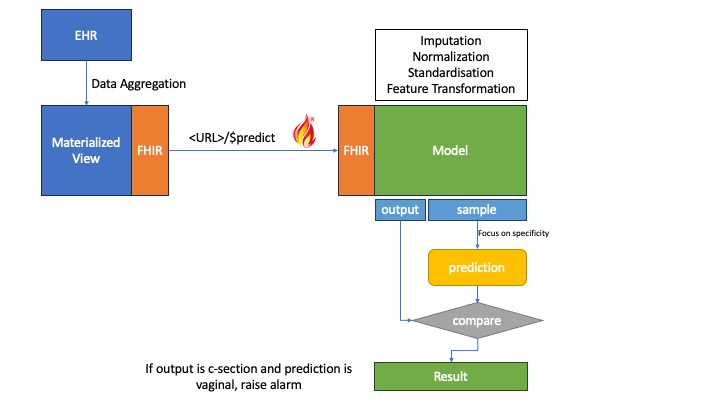
\includegraphics[scale=0.60]{figures/obs-model.jpg}
\end{figure}
%TC:endignore

\subsubsection{Clinical Evaluation}
The clinical evaluation was done by sending questionnaires to clinicians with a relationship with obstetrics in order to assess 10 patients, with only access to the variables used by the model and to answer 3 questions for each. The first was to give a score from 1-10 of how likely that patient would give birth through \ac{cs}, then to select the feature/variable that most influenced the decision and which feature they would require to make a better assessment. We sent the questionnaire to 20 people and got 6 answers. This rendered the results in figure \ref{fig:clinical}. We also predicted the result with the model as stated in figure \ref{fig:clinical}. These patients were new and not seen ever by the model in the training phase. 
As for the analysis of the most important features and missing features, the missing features were categorized into 3 categories: 1) Existent in the dataset but not included in the model, 2) Non-existent in the dataset and 3) existent in the dataset and included but that particular information was not filled for the patient assessed. This rendered a total of 62\% non-existent and 38\% existent but no information was provided at that moment. No feature mentioned existed but had not been included in the model. From the non-existent, 38\% were new clinical assessments, 38\% were linked to information from previous births,  15\% connected in more in-depth information about provided information (i.e, motive for induction) and 11\% were related to the mother's choice (if she wanted a \ac{cs}).
As for feature importance, from the 60 answers, we got 55\% with labour being the most important factor. 15\% answered the number of previous vaginal births, 8\% the evolution of weight and another 8\% the number of previous \acp{cs}. The remaining 14\% were various features, from \ac{bmi}, neuroaxis techniques, gestational age and weight of the mother. Of all of these, 90\% were included and were in the top 10 features of the model.



%TC:ignore

\begin{figure}[htbp]
\centering
\captionsetup{justification=centering}
\caption[Obstetrics questionnaires data]{Validation data. The colour represents the actual birth type. The boxplot represents the median and \ac{iqr} of the reviewers and the X represent each patient case. Contains 6 Vaginal births and 4 \acp{cs}. * represents wrong predictions of the model.}\label{fig:clinical} 
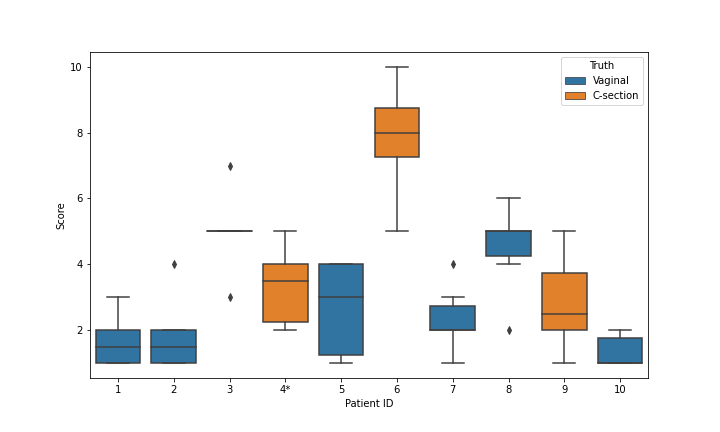
\includegraphics[scale=0.60]{figures/clinical_assessment.png}
\end{figure}
%TC:endignore


%TC:ignore

%\begin{figure}[htbp]
%\centering
%\captionsetup{justification=centering}
%\caption{Feature Importance of the model.}\label{fig:features} %
%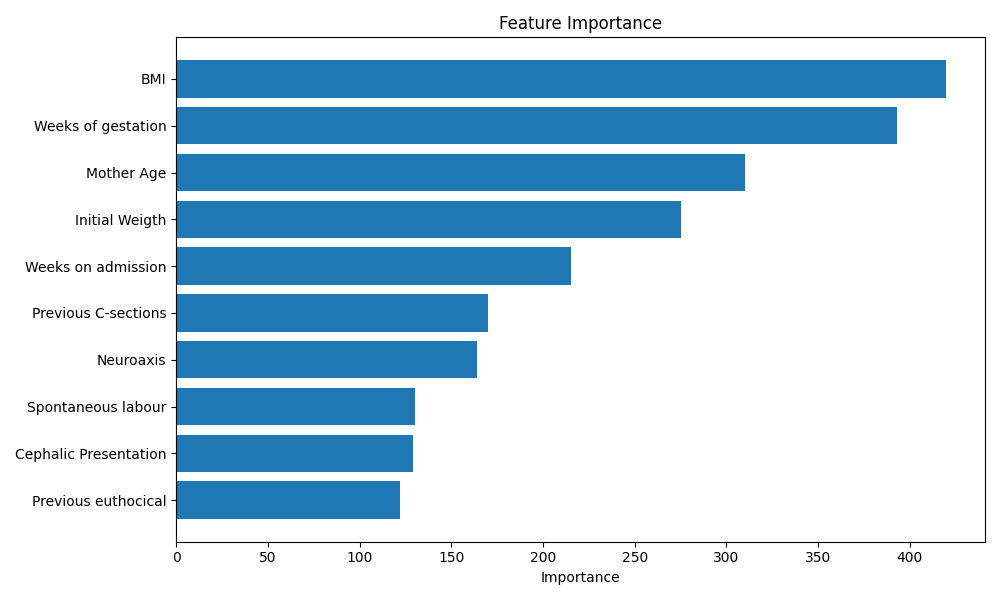
\includegraphics[scale=0.50]{figures/features.png}
%\end{figure}
%TC:endignore

\subsubsection{Potential Financial Impact}
The financial support provided to public hospitals in Portugal is partially tied to the rate of \acp{cs}. To assess the potential impact of this mechanism on all Portuguese public hospitals, we conducted a simulation study. We got data for every public hospital for the last 12 months \cite{pordatacesarianas} and applied a reduction of 3.8\% (the rate of warnings triggered in the new dataset) and recalculated the rate of \acp{cs}. The increase in support was calculated by the state-mandated rate as shown in table \ref{tab:corrections}. With this new rate, we observed that implementing our tool would result in financial benefits for 30\% (11 hospitals) of the public hospitals. Specifically, five hospitals would begin receiving support instead of no support at all. Three hospitals would experience a doubling of their financial benefit, while two hospitals would see a 50\% increase. Furthermore, one hospital would receive an additional one-third of financial support.
If we assumed that only half of the warnings found in the new data were actually true (1.9\%) we found that only 6 hospitals would be benefited. 3 from 0 to 0.25, 2 from 0.25 to 0.50 and 1 from 0.50 to 0.75.


\begin{table}[htbp]
  \centering
  \caption[Ruleset for financial support indexed to \acsp{cs}.]{Ruleset for state-provided financial support indexed to \acp{cs}. X is the current payment of a \ac{cs} inpatient episode. Adapted from \cite{acssTermosReferenciaPara2023}}
  \label{tab:corrections}
  \renewcommand{\arraystretch}{1.2} % Adjust the vertical spacing
  \setlength{\tabcolsep}{12pt} % Adjust the horizontal spacing
  \begin{tabular}{lc}
      \hline
Rate of \acp{cs}   & Support \\
    \hline
\textless 25\%       & x       \\
{[}25\%, 26.4\%{]}   & 0.75 x   \\
{[}26.5\%, 27.9\%{]} & 0.5 x    \\
{[}28\%, 29.4\%{]}   & 0.25 x   \\
\textgreater{}29,5\% & 0      \\
    \hline
\end{tabular}
\end{table}
    \subsection{Discussion}
    % !TeX root = ../../thesis.tex

The first thing to address about this model is the number of biases that we introduced in the model by choice. We joined all vaginal delivery types into a single category (assisted and non-assisted) which introduces a bias since these delivery modes are indeed different. Secondly, the fact that we want to predict if the delivery type was wrongly chosen, mainly for the case of a C-section that did not need to be so, is also a bias. We used this approach because the initially collected data did not have the representation of such events. So the biases of possibly wrong delivery types were present in the training data. We attempted to minimize this issue by selecting a threshold that gave the model higher sensitivity than specificity so that only large probabilities would trigger an alarm for human consideration. Parallel to this, we are starting to gather labelled cases, with the help of clinicians in order to create a better training dataset. Furthermore, since the data was collected from different hospitals, differences in the data input can also occur. Even though the health information system is the same, the processes that originate the data and are being used for secondary purposes could introduce several biases in the data. This is an issue that was accepted from the start regarding the mechanism of data collection and model training. Despite this, we reached a model with a very high \ac{auroc} (~88\%, 95\%CI [0.8795, 0.8815]), which is encouraging and versus the state of the art. Moreover, assuming that more data is provided and proper labelling is done regarding the outcome variable (like a clinical evaluation of needless C-sections) is added as well, a better model could be developed. Regarding the preliminary clinical evaluation, it was only possible to get an overview of the possible comparison due to the number of responders. Despite that, the results are encouraging, since the model seems to behave better than humans with the data provided. However, this is a biased vision, since clinicians in the real world have access to more data and information than the model has. It is encouraging, but caution is advised before more tests and evaluations are done. As for the deployment, future work could be the improvement of the \ac{api} in order to map all variables to an ontology like SNOMED CT or similar, making it easier for every system and person to access it and get a suggestion of the delivery type. Finally, we believe the assessment can be improved. A more robust clinical assessment is necessary as well as a thorough analysis of the impact of the tool in the real world, since we need to create the bridge between the results of the model and how clinical decisions are affected by it. A full cost-effectiveness analysis is also necessary to understand the real world impact of the model. One interesting result is the fact that 38\% of the answers regarding the most important data element missing from the patient record refers to data that is being collected but was missing for that specific patient, raising an important question about data input methodology, interoperability and quality. If we cannot have access to data when it matters most, it can become meaningless. Missing data is a problem of biomedical data as a whole. However, when specifically targeted at \ac{ml} usage of this data for predicting something, we did not find any works comparing them with clinicians. However, we did find reportsof similar missing values in obstetrics data \cite{venkateshMachineLearningStatistical2020} and we also found works of similar nature using \ac{ml} models with a robust handling of missing data such as \ac{xgboost} \cite{bitarMachineLearningAlgorithm2023} to counter this problem. This indicates that our model has the potential to counter the missing data problem as well since \ac{lightgbm} can also handle missing data natively.

    \subsection{Conclusion}
    We believe we have developed a robust system capable of detecting potentially incorrect C-section decisions, which could positively impact real-world medical practice. However, before implementation, several challenges must be addressed, particularly the need for further evaluation of the system's impact on clinical decision-making and the reasons underlying sub-optimal delivery type decisions. C-sections may be performed for various reasons, from a mother's preference to a decision made by the obstetrics team. This system is not designed to impede medical practice or to highlight flawed decisions, potentially scrutinizing specific professionals. Such caution is necessary when implementing systems like these. While having a high AUROC is beneficial, the real-world impact is another consideration. The assumptions and biases associated with autonomous systems supporting clinical practice must be carefully considered. Nonetheless, the metrics and results we have achieved so far are promising for positively influencing health and economic outcomes.
    
    
    
     
\begin{savequote}[75mm]
An expert is a person who has made all the mistakes that can be made in a very narrow field.
\qauthor{Niels Bohr}
\end{savequote}
\chapter{Conclusion and future work} \label{chap:conclusion}

\section{Limitations of the Studies}

\section{Conclusion}


\section{Recommendations for Future Research}
 
% !TeX root = ../thesis.tex

%\begin{savequote}[75mm]
%An expert is a person who has made all the mistakes that can be made in a very narrow field.
%\qauthor{Niels Bohr}

\begin{savequote}[75mm]
I may not have gone where I intended to go,
but I think I have ended up where I needed to be.
\qauthor{Douglas Adams}

\end{savequote}

\chapter{Conclusion} \label{chap:conclusion}
\initial{O}n a more personal note, I want to conclude this thesis, taking a step back and contemplate the work done so far. What I could have been done better and what I have learned throughout this journey.
But I also want to look ahead and point out possible directions in order to take the aim of this thesis further and create a substantial impact in the real world.

\section{Looking Back}
Reflecting on these last 5 years, the first impression that I get is shame regarding the earlier works in this thesis. While it bothered me at first, I now believe it is a sign of growth and maturity. I want to believe that is shows how much I have learned and grown. I also learned the value of collaboration and the importance of having a diverse team. I have learned that the most successful projects are those that embrace such interdisciplinary collaboration. Therefore, the future trajectory of this field may well hinge on fostering such diverse, collaborative environments, enriching the scope and impact of healthcare data science. Even though I always liked the saying of "if you want to go fast, go alone. If you want to go far, go together", I really never understood the importance of it until now. I have always tried to be a "one-man-show" but there are limits to this, whether time or knowledge-wise. \\

In contemplating the limitations of this thesis, it's pivotal to recognize that each project is inherently constrained by its unique focus and context. These projects were tailored to specific use cases and therefore may not offer broad generalizability. For instance, the work done in section \ref{subsec:obs} and \ref{subsec:distributed} are oriented around specific data types and formats and \ac{ml} models. Similarly, the project in \ref{subsec:dq} is circumscribed to a certain data type within a specific clinical specialty. This specificity implies that the outcomes of these projects might not be directly extrapolatable to other diseases or data types. However, it is crucial to note that the methodologies employed are versatile. For example, the real-time prediction techniques used in \ref{subsec:obs} and the data analysis models in \ref{subsec:ipop} and \ref{subsec:distributed} can be adapted for other contexts. Additionally, the \ref{subsec:similarity} method offers a versatile approach for analyzing diverse datasets and can be seamlessly integrated into various data pipelines.
But I cannot help to feel that the bigger limitation of this thesis is the lack of real-world deployment. While I have tried to simulate real-world scenarios, the lack of real-world deployment is a limitation. The deployment of real-world \ac{cdss} is, however, a complex undertaking requiring substantial investment in terms of time, finances, and perseverance. And of course, on top of this is the fact that we can bring problems to institutions and clinical workflow. Consequently, this aspect of tool deployment remains an avenue for future exploration. Nevertheless, extensive testing in real-world settings and the inclusion of clinicians in the developmental process imbue confidence in the readiness and potential impact of these tools upon deployment.



\section{Looking Ahead}
%focus on impact and application in real world. 
%TODO correct 

Looking towards future endeavors, the foundation established in this thesis paves the way for practical aid to healthcare teams. The deployment of real-world \ac{cdss} is, however, a complex undertaking requiring substantial investment in terms of time, finances, and perseverance. Consequently, this aspect of tool deployment remains an avenue for future exploration. Nevertheless, extensive testing in real-world settings and the inclusion of clinicians in the developmental process imbue confidence in the readiness and potential impact of these tools upon deployment.


The comprehensiveness of this work necessitated a confluence of knowledge from disparate domains. This included insights from biology and chemistry for understanding healthcare nuances, process design for process formalization, mathematics and statistics for \ac{ml} and Exploratory Data Analysis, and interoperability standards for data amalgamation. Furthermore, ethical and privacy considerations were paramount for ensuring patient confidentiality and developing ethically sound models. Delving into healthcare terminologies, codifications, and semantics was essential for data interpretation, along with familiarity with clinical specialties like obstetrics and oncology. Bridging the gap between \acp{rct} and observational or Real-World Data required adeptness in study design.

This multidisciplinary nature of the field underscores a key challenge: the necessity for a diverse skill set or, alternatively, a collaborative team with varied expertise. Our observations underscore that the most successful projects in this domain are those that embrace such interdisciplinary collaboration. Therefore, the future trajectory of this field may well hinge on fostering such diverse, collaborative environments, enriching the scope and impact of healthcare data science.
 


%% comment next 2 commands if numbered appendices are not used
\appendix
\chapter{} \label{ap1:loren}

\section{Data Dictionary}
\label{appendix:data_dict}
\begin{table}[H]
\renewcommand{\arraystretch}{0.58}
%\setlength{\tabcolsep}{14pt}
\begin{tabular}{ l   l }

\toprule
Acronym  &    Description \\
\midrule
IA &  Mother Age \\
GS  & Blood Group \\
PI &   Weight at the beginning of pregnancy \\
PAI &  Weight on Admission \\
IMC &   BMI \\
CIG &   If Smoker During Pregnancy \\
APARA  & Number of previously born babies\\
AGESTA  &   Number of Pregnancies   \\
EA &     Number of Previous Eutocic Deliveries with no assistance \\
VA &      Number of Previous Eutocic Deliveries with help of vacuum extraction \\
FA &     Number of Previous Eutocic Deliveries with help of forceps \\
CA &   Number of  Previous C-sections \\
TG &     Pregnancy Type (spontaneous, In vitro fertilisation...) \\
V &     If the pregnancy was accompanied by MD \\
NRCPN &     Number of prenatal consultations \\
VH &      If the pregnancy was followed by a MD in a hospital \\
VP &    If the pregnancy was followed by a MD in a private clinic \\
VCS &  If the pregnancy was followed by a MD in a primary care facility \\
VNH &    If the pregnancy was followed by a MD in the same hospital the delivery was made \\
B  & Pelvis Adequacy \\
AA & Baby's Position on Admission \\
BS &  Bishop Score \\
BC &   Bishop Score Cervical Consistency\\
BDE &  Bishop Score Fetal Station \\
BDI &  Bishop Score Dilatation \\
BE  &   Bishop Score Effacement \\
BP & Bishop Score Cervical Position \\
IGA  & Number of Weeks on Admission \\
TPEE  & If the delivery was spontaneous   \\
TPEI  &  If the delivery was induced  \\
RPM  & If there was a rupture of the amniotic pocket before delivery began \\
DG &  Gestational Diabetes \\
TP & Delivery Type \\
ANP  & Baby's Position on Delivery \\
TPNP  & Actual Type of Delivery\\
SGP  & Pregnancy Weeks on Delivery \\
GR  &   Robson Group \\
\bottomrule
\end{tabular}
\end{table}

%% questionarios
%% 

%%----------------------------------------
%% Final materials
%%----------------------------------------

%% Bibliography
%% Comment the next command if BibTeX file not used
%% bibliography is in ``myrefs.bib''

%\PrintBib{references, full-thesis}
%\bibliographystyle{plainnat}
\printbibliography
%% Index
%% Uncomment next command if index is required
%% don't forget to run ``makeindex thesis'' command
%% \PrintIndex

\end{document}
